\documentclass[12pt]{article}
% Some custom commands to make typing easier. Feel free to add to it


% quick homomorphism
\newcommand{\homo}[1]{\varphi (#1)}
% quick inverse
\newcommand{\inv}[1]{#1^{-1}}
% quick generating set
\newcommand{\genset}[1]{\langle #1 \rangle}
% split problem into multiple parts
\newcommand{\spl}{\rule{\textwidth}{0.4pt}}
% quick normal subgroup
\newcommand{\nsub}{\trianglelefteq}
% quick Z/nZ
\newcommand{\znz}[1]{\mathbb{Z\text{/#1}Z}}

% quick projective surface
\newcommand{\proj}[1]{\mathbb P^{#1}(\mathbb C)}
% quick elliptic curve
\newcommand{\ellip}{E(\mathbb{C})}
% quick ramification
\newcommand{\ram}[1]{e_{#1}}

% quick compactified complex plane
\newcommand{\Chat}{\widehat{\C}}

% todo list
\usepackage[color=yellow]{todonotes}
\newcommand{\tbd}[1]{\todo[inline]{#1}
\addcontentsline{toc}{subsubsection}{TODO}}

% scaling tikz
\usepackage{adjustbox}

% format bullets
% \usepackage[shortlabels]{enumitem}

% Document inherent packages to be loaded
\usepackage{amsmath, amsfonts, amssymb, amsthm, graphicx, url, xcolor, enumerate, tcolorbox}

%geometry helps manage margins, among other things.
\usepackage[rmargin=2in,lmargin=1in,tmargin=1in,bmargin=1in]{geometry}
\newcommand{\sidenote}[1]{\marginpar{\footnotesize \begin{itemize}
    \item[$\leftarrow$]\raggedright #1
\end{itemize}}}

\setlength{\headheight}{16pt}
\setlength{\marginparwidth}{1.5in}
\makeatletter      % make title smaller   
\def\@maketitle{   % custom maketitle 
\begin{center}
    {\Large \@title} \\[0.1in] \@author \\ {\small \@date}
\end{center}  
}
\setcounter{secnumdepth}{0}

\usepackage[colorlinks = true,
            linkcolor = teal,
            urlcolor  = teal,
            citecolor = teal,
            anchorcolor = teal]{hyperref}

\usepackage[all,2cell,ps]{xy}
\usepackage{tikz, tikz-cd}
\usepackage{faktor}
\allowdisplaybreaks
\graphicspath{{Images/}}

\theoremstyle{definition}  % to get rid of the italics
\newtheorem{theorem}{\bt{Theorem}}%[section]
\newtheorem{proposition}[theorem]{\bt{Proposition}}
\newtheorem{corollary}[theorem]{\gt{Corollary}}
\newtheorem{lemma}[theorem]{\bt{Lemma}}
\newtheorem{conjecture}[theorem]{Conjecture}

\newtheorem{defn}{\rt{Definition}}

\newtheorem{eg}{\textcolor{violet}{Example}}
\newtheorem{noneg}[eg]{\textcolor{violet}{Non-example}}

\newtheorem*{rmk}{Remark}


%Import the natbib package and sets a bibliography  and citation styles
\usepackage{natbib}

% Create headers
\usepackage{fancyhdr}
\usepackage{xcolor}
\renewcommand{\headrulewidth}{0pt}
\fancypagestyle{updated}{%
    \fancyhead{MATH135 Notes \hfill\hfill Xuehuai He}
    \fancyfoot{\hyperlink{toc}{Back to TOC}\hfill\thepage \hfill \textcolor{lightgray}{\today}}
}

% \newcommand{\Belyi}{Bely\u{\i}~}
% \newcommand{\thm}[3]{\vskip 0.2in \begin{center} \fbox{\begin{minipage}{0.8\linewidth} \begin{theorem}[#1] \label{#2} #3 \end{theorem} \end{minipage}} \end{center} \vskip 0.2in}
% \newcommand{\prop}[3]{\vskip 0.2in \begin{center} \fbox{\begin{minipage}{0.8\linewidth} \begin{proposition}[#1] \label{#2} #3 \end{proposition} \end{minipage}} \end{center} \vskip 0.2in}
% \newcommand{\cor}[3]{\vskip 0.2in \begin{center} \fbox{\begin{minipage}{0.8\linewidth} \begin{corollary}[#1] \label{#2} #3 \end{corollary} \end{minipage}} \end{center} \vskip 0.2in}
% \newcommand{\conj}[3]{\vskip 0.2in \begin{center} \fbox{\begin{minipage}{0.8\linewidth} \begin{conjecture}[#1] \label{#2} #3 \end{conjecture} \end{minipage}} \end{center} \vskip 0.2in}

\DeclareMathOperator{\Aut}{Aut}
\DeclareMathOperator{\Gal}{Gal}
\DeclareMathOperator{\Mon}{Mon}
\DeclareMathOperator{\lcm}{lcm}
\DeclareMathOperator{\Res}{Res}


\newcommand{\rt}[1]{\textcolor{magenta}{#1}}
\newcommand{\gt}[1]{\textcolor{olive}{#1}}
\newcommand{\bt}[1]{\textcolor{cyan}{#1}}

\newcommand{\N}{\mathbb{N}}
\newcommand{\Z}{\mathbb{Z}}
\newcommand{\C}{\mathbb{C}}
\newcommand{\R}{\mathbb{R}}
\newcommand{\Q}{\mathbb{Q}}
\newcommand{\F}{\mathbb{F}}
\newcommand{\D}{\mathbb{D}}
\newcommand{\reg}{\Omega}

\newcommand{\re}{\operatorname{Re}}
\newcommand{\im}{\operatorname{Im}}
\newcommand{\floor}[1]{\lfloor #1\rfloor}

\newcommand{\ifnif}{\textit{if and only if }}

\newcommand{\addlink}[1]{\addcontentsline{toc}{subsubsection}{#1}}

\newcommand{\circled}[1]{\begin{tikzpicture}[baseline=(word.base)]
\node[draw, rounded corners, text height=8pt, text depth=2pt, inner sep=2pt, outer sep=0pt, use as bounding box] (word) {#1};
\end{tikzpicture}
}

\newcommand{\ontangent}[1]{

    \spl

\textcolor{darkgray}{\textit{(Scratch work begins)}}
{#1}
\textcolor{darkgray}{\textit{(Scratch ends here)}}

\spl

}

\newcommand{\drawing}[2]{\begin{figure}[H]
    \centering
    \includegraphics[width=#1]{Images/#2}
\end{figure}}

\usepackage{pgfplots}
\pgfplotsset{compat=1.15}

\usepackage{ulem}
\usepackage{float}
\usepackage{libertinus}

% Make enumeration better
\usepackage{enumitem}
\setlist[itemize]{parsep=0pt,topsep=0pt}
\setlist[enumerate]{parsep=0pt,topsep=0pt}

% \definecolor{pomona}{HTML}{#0057b8}

\parskip = .2in
\parindent = 0in

% clever ref (load last)
\usepackage[capitalise]{cleveref}
\newcommand{\fref}{\cref}
\newcommand{\Fref}{\Cref}
\newcommand{\prettyref}{\cref}
\newcommand{\newrefformat}[2]{}

 %Cleveref definitions
\crefname{lemma}{Lemma}{Lemmas}
\crefname{thm}{Theorem}{Theorems}
\crefname{defn}{Definition}{Definitions}
\crefname{notn}{Notation}{Notations}
\crefname{const}{Construction}{Constructions}
\crefname{prop}{Proposition}{Propositions}
\crefname{rem}{Remark}{Remarks}
\crefname{cor}{Corollary}{Corollaries}
\crefname{equation}{Equation}{Equations}
\crefname{ex}{Example}{Examples}
\renewcommand{\d}{\ensuremath{\operatorname{d}}}

%=============

\begin{document}
\title{MATH135 Complex Analysis Notes}
\author{Xuehuai He}
\maketitle

\hypertarget{toc}{}
{\parskip=0.05in
\tableofcontents}

\spl

\newpage
\pagestyle{updated}

\section{Regions, differentiability, analyticity}

\subsection{Regions}
\defn A \textbf{region} is a \uline{nonempty, connected, open subset} of $\C$.
\begin{itemize}
    \item A region without ``holes'' is \uline{simply connected}.
\end{itemize}

\noneg This is not a region (not connected): \drawing{80pt}{image.png}

\eg $\C$ is a region.
\eg $\mathbb{D} = \{z\in \C\mid |z|<1\}$, the open unit disk is a region.
\eg $\{z\in \C \mid 1<|z|<2\}$, the annulus region is a region that is not \textit{simply-connected}:\drawing{80pt}{image-1.png}

\subsection{Complex derivatives and analyticity}

\defn Let $\reg$ be a region. Let $z_0\in \reg$ and $f:\reg \to \C$ be a function.
\begin{enumerate}
    \item Complex function $f$ is \textbf{differentiable} \sidenote{this $z\to z_0$ could be from \textbf{any} directions!}at $z_0$ if \begin{align*}
        f'(z_0)=\lim_{z\to z_0}\frac{f(z)-f(z_0)}{z-z_0}
    \end{align*}
    exists.

    \item If $f$ is differentiable at every point in $\reg$, we say $f$ is \textbf{analytic} on $\reg$.\sidenote{Means that existence of 1st derivative implies the existence of $\infty$th derivative! \& has Taylor expansion.}
    \item If $f$ is analytic on $\C$, then $f$ is \textbf{entire}.
\end{enumerate}
\sidenote{Usual calculus rules work here :)}

\eg Polynomials are entire functions.
\eg Rational functions are analytic on $\C$ except where the denominator vanishes.
\noneg $f(z)=\bar z$ is NOT analytic \textbf{anywhere}!
\begin{proof}
    Let $z_0\in \C$. Then $\frac{f(z)-f(z_0)}{z-z_0}=\frac{\bar z-\bar z_0}{z-z_0}$.

    If $z\to z_0$ horizontally, then $z-z_0\in \R$, meaning that $$\lim_{z\to z_0}=\frac{f(z)-f(z_0)}{z-z_0}=\frac{\bar z-\bar z_0}{z-z_0}=\frac{z-z_0}{z-z_0}=1.$$

    Else if $z\to z_0$ vertically, then $\overline{z-z_0}=-(z-z_0)$, meaning that $$\lim_{z\to z_0}=\frac{f(z)-f(z_0)}{z-z_0}=\frac{\bar z-\bar z_0}{z-z_0}=\frac{-(z-z_0)}{z-z_0}=-1.$$

    We observe that $1\neq -1$, thus, the limit from different directions are not the same. We conclude that the limit does not exist anywhere.
\end{proof}

\begin{proposition}\label[proposition]{epsilon-delta-limit}
    Let $f$ be differentiable at $z_0$. Then, for any $\varepsilon >0$, there exists some $\delta>0$ such that \textbf{whenever} $0<|z-z_0|<\delta$, \textbf{we have} $|f'(z_0)-\frac{f(z)-f(z_0)}{z-z_0}|<\varepsilon$.
\end{proposition}

\rmk Now consider multiplying $|z-z_0|$ on both sides of \cref{epsilon-delta-limit}:\begin{align*}
    |f'(z_0)\cdot (z-z_0) - f(z) + f(z_0)| &< \varepsilon |z-z_0|\\
    |f(z_0) + f'(z_0)(z-z_0)-f(z)| &<\varepsilon |z-z_0|
\end{align*}

That is to say, near $z_0$ (when the distance $<\varepsilon$), \begin{align*}
    f(z)≈f(z_0) + f'(z_0)(z-z_0)
\end{align*}\sidenote{The RHS is a \textbf{linear} function!}
this is the ``tangent-line approximation'' equivalent in $\C$!

In addition, $f(z_0) + f'(z_0)(z-z_0)$ means to take $z-z_0$, rotate and dilate by $f'(z_0)$, then translate by $f(z_0)$. If $f'(z_0)\neq 0$, this function is \uline{locally orientation-preserving} and could be approximated by a linear function.\sidenote{This explains why $z\mapsto \bar z$ is NOT analytic anywhere: it is orientation-reversing.}

\subsection{Curves, paths}

\defn A \textbf{curve} in $\C$ is a function $\gamma: [a,b]\to \C, a,b\in \R$.
\[
    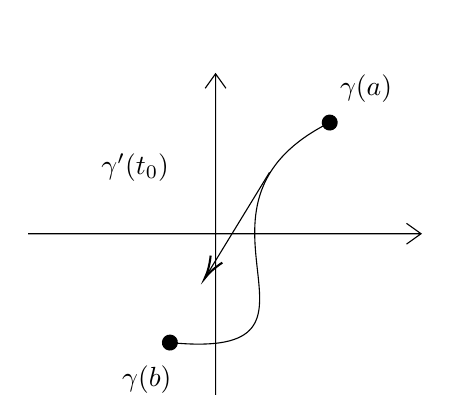
\begin{tikzpicture}[x=0.75pt,y=0.75pt,yscale=-1,xscale=1]
        %uncomment if require: \path (0,286); %set diagram left start at 0, and has height of 286
        
        %Shape: Axis 2D [id:dp5992461788507699] 
        \draw  (50,141.08) -- (239.26,141.08)(140.26,64) -- (140.26,226.51) (232.26,136.08) -- (239.26,141.08) -- (232.26,146.08) (135.26,71) -- (140.26,64) -- (145.26,71)  ;
        %Curve Lines [id:da8169369769076535] 
        \draw    (118.26,193.51) .. controls (210.26,202.51) and (113.26,128.51) .. (195.26,87.51) ;
        \draw [shift={(195.26,87.51)}, rotate = 333.43] [color=black  ][fill=black  ][line width=0.75]      (0, 0) circle [x radius= 3.35, y radius= 3.35]   ;
        \draw [shift={(118.26,193.51)}, rotate = 5.59] [color=black  ][fill=black  ][line width=0.75]      (0, 0) circle [x radius= 3.35, y radius= 3.35]   ;
        %Straight Lines [id:da7279313778056917] 
        \draw    (166.26,111.51) -- (136.05,160.92) ;
        \draw [shift={(135,162.63)}, rotate = 301.44] [color=black  ][line width=0.75]    (10.93,-3.29) .. controls (6.95,-1.4) and (3.31,-0.3) .. (0,0) .. controls (3.31,0.3) and (6.95,1.4) .. (10.93,3.29)   ;
        
        % Text Node
        \draw (199,63.4) node [anchor=north west][inner sep=0.75pt]    {$\gamma ( a)$};
        % Text Node
        \draw (94,203.4) node [anchor=north west][inner sep=0.75pt]    {$\gamma ( b)$};
        % Text Node
        \draw (84,101.4) node [anchor=north west][inner sep=0.75pt]    {$\gamma '( t_{0})$};
        
        
        \end{tikzpicture}
\]

\defn Parameterize $\gamma(t)=(x(t), y(t))=x(t)+iy(t)$. Then $\gamma'(t_0)=(x'(t_0), y'(t_0))$ is a \textbf{tangent vector} to the curve at $\gamma(t_0)$ (assume $\gamma'(t_0)\neq \mathbf{0}$, aka. $\gamma$ is regular at $\gamma(t_0)$.)

\begin{theorem}[The ``Boxy-path'' Theorem]
    A nonempty open set $\Omega$ in $\C$ is connected \textit{if and only if} each pair of distinct
points in $\Omega$ can be joined by a sequence of line segments lying in $\Omega$, each of which is
parallel to either to the real or imaginary axis.
    \drawing{0.6\linewidth}{image-3.png}
    In other words, between any 2 points in a region $\reg$ there exists a ``\textbf{boxy path}''.
\end{theorem}

\rmk There is also always a \textbf{smooth path}. That is: \drawing{150pt}{image-4.png}

\begin{theorem}[``Smooth-path'']
    A nonempty open set $\reg$ in $\C$ is connected if and only if each pair of distinct
points in $\reg$ can be joined by a continuously differentiable curve in $\reg$ that is regular at
every point.
\end{theorem}
\begin{proof}
    See \href{https://stephangarcia.sites.pomona.edu/teaching/24S-135/Lecture/24S-135-Lecture02.pdf}{lecture 2 notes}.
\end{proof}

\subsection{Conformality}
Let $f$ be an analytic complex function on $\reg$.

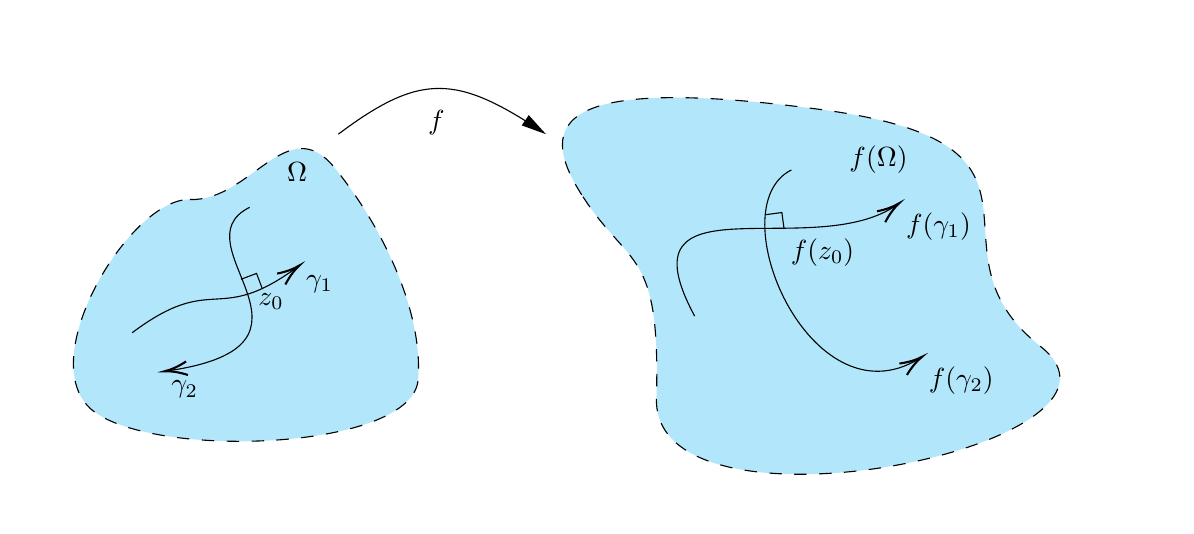
\begin{tikzpicture}[x=0.75pt,y=0.75pt,yscale=-1,xscale=1]
    %uncomment if require: \path (0,300); %set diagram left start at 0, and has height of 300
    
    %Shape: Polygon Curved [id:ds04152892949921583] 
    \draw  [fill=cyan  ,fill opacity=0.3 ][dash pattern={on 4.5pt off 4.5pt}] (92.5,102.5) .. controls (121.5,103.5) and (139.5,59.5) .. (162,87) .. controls (184.5,114.5) and (204.91,155.75) .. (202.42,189.25) .. controls (199.92,222.75) and (79.59,227.75) .. (47.08,205.25) .. controls (14.58,182.75) and (63.5,101.5) .. (92.5,102.5) -- cycle ;
    %Curve Lines [id:da38490573070321243] 
    \draw    (64.67,166.67) .. controls (104.27,136.97) and (105.24,163.7) .. (144.07,135.13) ;
    \draw [shift={(145.25,134.25)}, rotate = 143.13] [color=black  ][line width=0.75]    (10.93,-3.29) .. controls (6.95,-1.4) and (3.31,-0.3) .. (0,0) .. controls (3.31,0.3) and (6.95,1.4) .. (10.93,3.29)   ;
    %Curve Lines [id:da9683797356751562] 
    \draw    (121.25,106.25) .. controls (85.43,124.16) and (167.43,172.76) .. (81.56,185.07) ;
    \draw [shift={(80.25,185.25)}, rotate = 352.23] [color=black  ][line width=0.75]    (10.93,-3.29) .. controls (6.95,-1.4) and (3.31,-0.3) .. (0,0) .. controls (3.31,0.3) and (6.95,1.4) .. (10.93,3.29)   ;
    %Shape: Right Angle [id:dp0014762610750393979] 
    \draw   (117.1,140.91) -- (124.59,138.1) -- (127.4,145.59) ;
    %Shape: Polygon Curved [id:ds020760136591730705] 
    \draw  [fill=cyan  ,fill opacity=0.3 ][dash pattern={on 4.5pt off 4.5pt}] (281.25,100.25) .. controls (258.25,64.25) and (271.25,42.25) .. (397.25,59.25) .. controls (523.25,76.25) and (442.25,126.25) .. (502.25,173.25) .. controls (562.25,220.25) and (315.25,271.25) .. (317.25,198.25) .. controls (319.25,125.25) and (304.25,136.25) .. (281.25,100.25) -- cycle ;
    %Curve Lines [id:da5067199553805877] 
    \draw    (335.67,158.67) .. controls (298.63,89.94) and (392.35,133.36) .. (433.04,105.13) ;
    \draw [shift={(434.25,104.25)}, rotate = 143.13] [color=black  ][line width=0.75]    (10.93,-3.29) .. controls (6.95,-1.4) and (3.31,-0.3) .. (0,0) .. controls (3.31,0.3) and (6.95,1.4) .. (10.93,3.29)   ;
    %Curve Lines [id:da12902529814050778] 
    \draw    (382.25,88.25) .. controls (346.61,106.07) and (391.34,211.12) .. (443.67,179.26) ;
    \draw [shift={(445.25,178.25)}, rotate = 146.56] [color=black  ][line width=0.75]    (10.93,-3.29) .. controls (6.95,-1.4) and (3.31,-0.3) .. (0,0) .. controls (3.31,0.3) and (6.95,1.4) .. (10.93,3.29)   ;
    %Shape: Right Angle [id:dp16473621622546486] 
    \draw   (369.76,109.81) -- (377.69,108.76) -- (378.75,116.69) ;
    %Curve Lines [id:da7241992906101147] 
    \draw    (164,71) .. controls (203.6,41.3) and (220.91,42.23) .. (262.73,70.15) ;
    \draw [shift={(264,71)}, rotate = 213.92] [fill=black  ][line width=0.08]  [draw opacity=0] (12,-3) -- (0,0) -- (12,3) -- cycle    ;
    
    % Text Node
    \draw (138,83.4) node [anchor=north west][inner sep=0.75pt]    {$\Omega $};
    % Text Node
    \draw (147.25,137.65) node [anchor=north west][inner sep=0.75pt]    {$\gamma _{1}$};
    % Text Node
    \draw (82.25,188.65) node [anchor=north west][inner sep=0.75pt]    {$\gamma _{2}$};
    % Text Node
    \draw (124.25,146.65) node [anchor=north west][inner sep=0.75pt]    {$z_{0}$};
    % Text Node
    \draw (409,75.4) node [anchor=north west][inner sep=0.75pt]    {$f( \Omega )$};
    % Text Node
    \draw (436.25,107.65) node [anchor=north west][inner sep=0.75pt]    {$f( \gamma _{1})$};
    % Text Node
    \draw (447.25,181.65) node [anchor=north west][inner sep=0.75pt]    {$f( \gamma _{2})$};
    % Text Node
    \draw (380.75,120.09) node [anchor=north west][inner sep=0.75pt]    {$f( z_{0})$};
    % Text Node
    \draw (206,58.4) node [anchor=north west][inner sep=0.75pt]    {$f$};
    
    
\end{tikzpicture}

Let $z_0\in \reg$ such that $f'(z_0)\neq 0$. Let $\gamma_1, \gamma_2$ be two curves that pass through $z_0$ intersecting with an angle $\theta$. Then $f(\gamma_1), f(\gamma_2)$ are two curves in $f(\Omega)$ passing through $f(\zeta_0)$ also with angle $\theta$.

Therefore, $f$ is \textbf{conformal}!

\section{Cauchy-Riemann equations, harmonic functions}
\subsection{Multivariate notion of complex derivatives}
Recall: $\displaystyle f'(z_0)=\lim_{h\to 0}\frac{f(z_0+h)-f(z_0)}{h}$.

Now we write each function with complex variables as $f(z)=u(z)+i\, v(z)$ where $u,v$ are real-valued \sidenote{meaning their range is real} functions.

Since $\C\cong \R^2$, we denote every point $z=(x,y)$.

Now we let $f(x,y)=u(x,y)+i\,v(x,y)$. We first let the small distance $h=(r,0)$ be horizontally approaching 0 with $r\in \R$. That is, $z_0+h=(x_0+r,y_0)$.
\begin{align*}
    f'(z_0) &= \lim_{r\to 0} \frac{u(x_0+r, y_0)-u(x_0,y_0)}{r} + i\cdot \lim_{r\to 0}\frac{v(x_0+r, y_0)-v(x_0,y_0)}{r}\\
    &=u_x(x_0,y_0)+i\cdot v_x(x_0,y_0)
\end{align*}

Similarly, if we vertically let $h=ir=(0,r)$ with $r\to 0, r\in \R$, we would get $f'=v_y-i\cdot u_y$.

\rmk If a derivative exists, the horizontal \& the vertical ones should be equal!

\begin{theorem}[Cauchy-Riemann Equations]
    \begin{align*}
        u_x &=v_y\\
        u_y &= -v_x
    \end{align*}
\end{theorem}\addlink{Cauchy-Riemann Equations}

\begin{corollary}
    If $f:\reg \to \C$ is analytic and $f'=0$ on $\reg$, then $f$ is \textbf{constant}.
\end{corollary}
\begin{proof}
    Since $0=f'=u_x+iv_x$, we see that $u_x=v_x=0$ on $\reg$. By Cauchy-Riemann, $v_y=u_y=0$ is also true on $\reg$. Hence, $\mathbf{u}, \mathbf{v}$ are constant on either horizontal or vertical segments. By the Boxy Path Theorem, $f=u+iv$ cannot assume two distinct values in $\reg$.
\end{proof}

\subsection{Orientation-preserving as shown by Jacobian}
Let $f:\reg \to \C$ be analytic. Then $f'=u_x+iv_x$ and hence:\begin{align*}
    |f'|^2 = \bar f'\cdot f &= (u_x-iv_x)(u_x+iv_x)\\
    &= u_x^2 + v_x^2\\
    &= u_xu_x+v_xv_x && \text{and by Cauchy-Riemann,}\\
    &= u_xv_y-u_yv_x\\
    &= \det\left(\begin{bmatrix}
        u_x & u_y\\
        v_x & v_y
    \end{bmatrix}\right) && \text{the Jacobian of $f$!}
\end{align*}

Since $|f'|^2\geq 0$, the determinant of the Jacobian is always $\geq 0$, implying that $f$ is always locally orientation-preserving. Moreover,

\begin{proposition}
    If $f'(z_0)\neq 0$, then $|f'|^2> 0$ implies:
    \begin{enumerate}
        \item $f$ is \textbf{injective} near $z_0$
        \item $f$ scales $\R$ by $|f'(z_0)|^2$ near $z_0$
        \item $f$ preserves orientation near $z_0$
    \end{enumerate}
\end{proposition}

\subsection{The Laplacian, harmonic functions and conjugates}
Suppose that $f=u+iv$ is analytic and $u,v$ have continuous second partial derivatives. Then:\begin{align*}
    u_{xx}+u_{yy} = \Delta u = (v_y)_x + (-v_x)_y = v_{yx}-v_{xy}=0
\end{align*}
This means that the Laplacian of this function $u$ is 0!\sidenote{$\Delta u = 0$ characterizes steady-state solutions to heat equations on $\reg$.}

\defn Real-valued functions $u: \reg\to \R$ satisfying that the Laplacian $\Delta u= u_{xx}+u_{yy}$ is 0 on $\reg$ is called \textbf{harmonic functions}.

\defn A \textbf{harmonic conjugate} of $u$ is a harmonic function $v: \reg \to \R$ such that $f=u+i\cdot v$ is \textbf{analytic} on $\reg$.
\addlink{Harmonic conjugate}

\eg $u=x^2-y^2, v=2xy$.\sidenote{Check it!}

\rmk Harmonic conjugates are unique up to translation (± constants).

\rmk If $u$ is harmonic on $\reg$, it does NOT have to have a harmonic conjugate on $\reg$.

\subsection{Finding a harmonic conjugate}
Recall that the real and imaginary parts of an analytic function are \textbf{harmonic}, in addition to satisfying the Cauchy-Riemann Equations: $u_x=v_y$ and $u_y=-v_x$.

\eg $u(z)=\log |z|$ is harmonic on $\C\backslash\{0\}$.
\begin{proof}
    Write $u(x,y)=\log (\sqrt{x^2+y^2})=\frac{1}{2}\log(x^2+y^2)$.

    Then, \begin{align*}
        u_x&=\frac{\partial}{\partial x}\left(\frac{1}{2}\log (x^2+y^2)\right)\\
        &= \frac{1}{2}\cdot \frac{2x}{x^2+y^2}\\
        &= \frac{x}{x^2+y^2}
    \end{align*}

    Hence,\sidenote{Review quotient rule!}
    \begin{align*}
        u_{xx} &= \frac{(x^2+y^2)-x(2x)}{(x^2+y^2)^2}\\
        &= \frac{y^2-x^2}{(x^2+y^2)^2}
    \end{align*}

    Symmetrically, we find \begin{align*}
        u_{yy} & = \frac{x^2-y^2}{(x^2+y^2)^2}
    \end{align*}
    Hence $u_{xx}+u_{yy}=0$, implying that the function is harmonic.
\end{proof}

Now, can we \uline{find a harmonic conjugate for the aforementioned $u$}?\sidenote{There is currently a great \textbf{CAVEAT} in all of these, because $v(z)=\arg(z)$ cannot be defined in a continuous manner in all of $\C\backslash\{0\}$: 

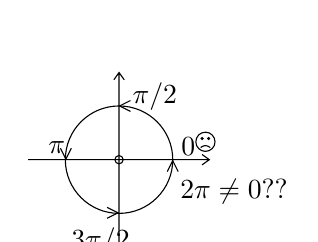
\begin{tikzpicture}[x=0.75pt,y=0.75pt,yscale=-0.5,xscale=0.5]
    %uncomment if require: \path (0,300); %set diagram left start at 0, and has height of 300
    
    %Shape: Axis 2D [id:dp48156480156165227] 
    \draw  (111,139) -- (285.5,139)(198.5,55) -- (198.5,219) (278.5,134) -- (285.5,139) -- (278.5,144) (193.5,62) -- (198.5,55) -- (203.5,62)  ;
    %Shape: Circle [id:dp6012967995903811] 
    \draw   (146.75,139) .. controls (146.75,110.42) and (169.92,87.25) .. (198.5,87.25) .. controls (227.09,87.25) and (250.26,110.42) .. (250.26,139) .. controls (250.26,167.58) and (227.09,190.75) .. (198.5,190.75) .. controls (169.92,190.75) and (146.75,167.58) .. (146.75,139) -- cycle ;
    \draw   (209.5,92.5) -- (199,87.25) -- (209.5,82) ;
    \draw   (152.5,128) -- (147.25,138.5) -- (142,128) ;
    \draw   (187,185) -- (197.5,190.25) -- (187,195.5) ;
    \draw   (245,150.5) -- (250.25,140) -- (255.5,150.5) ;
    %Shape: Smiley Face [id:dp013237994815757492] 
    \draw   (272.5,121.75) .. controls (272.5,116.64) and (276.64,112.5) .. (281.75,112.5) .. controls (286.86,112.5) and (291,116.64) .. (291,121.75) .. controls (291,126.86) and (286.86,131) .. (281.75,131) .. controls (276.64,131) and (272.5,126.86) .. (272.5,121.75) -- cycle ; \draw   (277.68,118.61) .. controls (277.68,118.09) and (278.09,117.68) .. (278.61,117.68) .. controls (279.12,117.68) and (279.53,118.09) .. (279.53,118.61) .. controls (279.53,119.12) and (279.12,119.53) .. (278.61,119.53) .. controls (278.09,119.53) and (277.68,119.12) .. (277.68,118.61) -- cycle ; \draw   (283.97,118.61) .. controls (283.97,118.09) and (284.38,117.68) .. (284.9,117.68) .. controls (285.41,117.68) and (285.82,118.09) .. (285.82,118.61) .. controls (285.82,119.12) and (285.41,119.53) .. (284.9,119.53) .. controls (284.38,119.53) and (283.97,119.12) .. (283.97,118.61) -- cycle ; \draw   (277.13,127.3) .. controls (280.21,124.83) and (283.29,124.83) .. (286.38,127.3) ;
    %Shape: Circle [id:dp5943162664556252] 
    \draw   (194.51,139) .. controls (194.51,136.79) and (196.3,135) .. (198.5,135) .. controls (200.71,135) and (202.5,136.79) .. (202.5,139) .. controls (202.5,141.21) and (200.71,143) .. (198.5,143) .. controls (196.3,143) and (194.51,141.21) .. (194.51,139) -- cycle ;
    
    % Text Node
    \draw (256,115.4) node [anchor=north west][inner sep=0.75pt]    {$0$};
    % Text Node
    \draw (209,62.4) node [anchor=north west][inner sep=0.75pt]    {$\pi /2$};
    % Text Node
    \draw (128,119.4) node [anchor=north west][inner sep=0.75pt]    {$\pi $};
    % Text Node
    \draw (150,202.4) node [anchor=north west][inner sep=0.75pt]    {$3\pi /2$};
    % Text Node
    \draw (255,155.4) node [anchor=north west][inner sep=0.75pt]    {$2\pi \neq 0??$};
    
    
    \end{tikzpicture}
    

To be resolved later!}

We could use the two Cauchy-Riemann Equations. One of them:
\begin{align*}
    v_y&=u_x\\
    &= \frac{x}{x^2+y^2}
\end{align*}
Therefore, \begin{align*}
    v(x,y) &= \int v_ydy + C(x) && \text{unknown function of }x\\
    &= \arctan\left(\frac{y}{x}\right)+C(x)
\end{align*}

Then, we use the second one: \begin{align*}
    \frac{y}{x^2+y^2}=u_y=-v_x &= -\frac{\partial}{\partial x} \left( \arctan\left(\frac{y}{x}\right)+C(x)\right)\\
    &= \frac{y}{x^2+y^2}-C'(x) \implies C'(x)=0
\end{align*}

Hence, a good harmonic conjugate candidate seems to be \begin{align*}
    v(x,y) = \arctan\left(\frac{y}{x}\right) + C
\end{align*}
where $C$ is a constant. WLOG, let $C=0$. Then $ v(x,y)=\arctan\left(\frac{y}{x}\right)$, meaning that: \begin{align*}
    v(z)=\arg (z)
\end{align*}

Therefore, $f(z)=\log |z| + i\cdot \arg(z)$ is analytic!
%%%%%%%

\subsection{Physics analogies of harmonic functions}
\eg Let $T(x,y,t)$ be the temperature at $(x,y)$ at time $t$ of a thermally conductive plate in $\C$. Assume the plate gives rise to a \textbf{bounded} region $\Omega$ (with boundary denoted $\partial \Omega$). Temperature on $\partial \Omega$ is a fixed function (time-independent).

\begin{figure}[H]
    \centering
    
\includegraphics[width=80pt]{Images/image-2.png}
\end{figure}

Now given the heat equation: \begin{align*}
    \frac{\partial T}{\partial t}-\alpha \Delta T=0
\end{align*}
where $\alpha$ is a constant.

We think the system tends towards a thermal equilibrium as $t\to \infty$. At equilibrium, $\frac{\partial T}{\partial t}$ is \textbf{zero}. Hence, at equilibrium, $\Delta T=T_{xx}+T_{yy}=0$.

\textbf{\underline{Idea}}: \hypertarget{physics}{Harmonic function behave like equilibrium temperature distributions!}

\begin{proposition}
    Let $U(x,y)$ be a harmonic function on $\Omega$.
    \begin{enumerate}
        \item $U$ cannot have a \textit{local} maximum in $\Omega$.
        \item The absolute maximum of $U$ on $\Omega ^-$\sidenote{$\Omega ^-$ denotes the closure of $\Omega$} occurs on $\partial \Omega$.
        \item $U$ cannot be locally constant without being globally constant.
    \end{enumerate}
\end{proposition}

\begin{theorem}[Maximum principle]
    Let $\Omega$ be a bounded region in $\C$ and let $f: \Omega^-\to \C$ be analytic on $\Omega$ and continuous on $\Omega^-$.
    \begin{enumerate}
        \item If $|f|$ achieves a local max in $\Omega$, then $f$ is constant.
        \item The global max of $|f|$ on $\Omega^-$ is attained on $\partial \Omega$.
    \end{enumerate}
\end{theorem}

\section{Möbius transformations}
\subsection{Möbius transformations, the extended plane}
\defn[Möbius transformations]
\begin{align*}
    f(z)=\frac{az+b}{cz+d}\text{ where } ad-bc\neq 0, a,b,c,d\in \C
\end{align*}
Such an $f$ is \textbf{analytic} on $\C\backslash\{\frac{-d}{c}\}$\sidenote{recall that rational functions are analytic except when the denominator vanishes, i.e. $cz+d\neq 0$.} and \textbf{comformal} there since $f'(z)=\frac{ad-bc}{(cz+d)^2}\neq 0$ on $\C\backslash\{\frac{-d}{c}\}$.

\rmk In addition, $f$ is injective (one-to-one)!
\begin{proof}
    \begin{align*}
        f(z)=f(w)\implies \frac{az+b}{cz+d}&=\frac{aw+b}{cw+d}\\
         (az+b)(cw+d)&= (cz+d)(aw+b)\\
         aczw+bcw+adz+bd&=aczw+adw+bcz+bd\\
         (ad-bc)z&=(ad-bc)w\\
         z&=w
    \end{align*}
\end{proof}

\defn[The extended plane] We set the following convention:\begin{align*}
    f(\frac{-d}{c})&= \infty\\
    f(\infty) &= \frac{a}{c}
\end{align*}
with this, $f$ is a \textbf{bijection} from $\Chat=\C\cup\{\infty\}$ to itself.\sidenote{recall Riemann sphere}

\subsection{Möbius transformations as matrices}
\rmk We can \textit{associate}\sidenote{this association is not a bijection: it's only so up to scaling} $f(z)=\frac{az+b}{cz+d}$ where $ad-bc\neq 0$ with the matrix $$M_f=\begin{bmatrix}
    a&b\\c&d
\end{bmatrix}$$

\rmk $M_{f\circ g}=M_f\cdot M_g$\sidenote{check this!}

\rmk The inverse of $M_f=\begin{bmatrix}
    a&b\\c&d
\end{bmatrix}$ is $M_f^{-1}=\frac{1}{ad-bc}\begin{bmatrix}
    d&-b\\-c&a
\end{bmatrix}$ and scaling does not matter, so we could write the \textbf{inverse} of such Möbius transformation as: \begin{align*}
    \inv{f}(w) &=\frac{dw-b}{-cw+a}
\end{align*}

\begin{theorem}
    A Möbius transformation $f:\Chat\to\Chat$ with three fixed points in $\Chat$ is the \textbf{identity map} $\mathrm{id}(z)=z=\frac{z+0}{0z+1}$.\sidenote{$I=\begin{bmatrix}
        1&0\\0&1
    \end{bmatrix}$}
\end{theorem}
\begin{proof}
    Let $f(z)=\frac{az+b}{cz+d}$ be a Möbius transformation.
    \begin{enumerate}
        \item If $\infty$ is fixed, then $c=0$\sidenote{think about that!}. Then $f(z)=\frac{a}{d}z+\frac{b}{d}$, which is a \textbf{linear} transformation.\begin{enumerate}
            \item If $f(z)=z$, we are done since we get the identity!
            \item Otherwise the function only has one fixed point at $\infty$.
        \end{enumerate}
        \item If $\infty$ is not a fixed point, then $c\neq 0$. Solve:\begin{align*}
            f(z)+z \Leftrightarrow \frac{az+b}{cz+d}&=z\\
            az+b&=cz^2+dz\\
            cz^2+(d-a)z-b&=0
        \end{align*}
        is a quadratic which has at most two (distinct) solutions in $\C$. Hence, this transformation fixes at most two points.
    \end{enumerate}
\end{proof}

\subsection{Möbius transformations take circles to circles}
\rmk Lines can be circles (they are just circles that pass through the point at infinity).

\begin{theorem}
    The image of a circle under a Möbius transformation is still a circle.
\end{theorem}
\begin{proof}
    Let $f(z)=\frac{az+b}{cz+d}$ be a Möbius transformation.
    \begin{enumerate}
        \item If $c=0$, then $f(z)=\frac{a}{d}z+\frac{b}{d}$, which is a \textbf{linear/affine} transformation and so we are done\sidenote{since linear transformations preserve circles and lines}.
        \item Now suppose $c\neq 0$. Then \begin{align*}
            f(z)&=\frac{a}{d}z+\frac{b}{d}\\
            &= \frac{\frac{a}{c}(cz+d)-\frac{ad}{c}+b}{cz+d}\\
            &= \frac{b-\frac{ad}{c}}{cz+d}+\frac{a}{c}
        \end{align*}
        which is a composition of affine, inversion and affine:
        $$z\mapsto cz+d\mapsto \frac{1}{cz+d}\mapsto \frac{b-\frac{ad}{c}}{cz+d}+\frac{a}{c}$$
        We now only need to show that inversion preserves circles.

        Let a circle in $\R^2$ be $Ax+By+C(x^2+y^2)=D$ where $A,B,C,D\in \R$. If $z=x+iy\in \Chat$, then $\frac{1}{z}=\frac{x}{x^2+y^2}+i\frac{-y}{x^2+y^2}$. Name $\frac{1}{z}=u+iv$, note that $u^2+v^2=\frac{1}{x^2+y^2}$. 
        
        Then we note that $Au-Bv+C=D(u^2+v^2)$\sidenote{check this!}, which is still a circle!
    \end{enumerate}
\end{proof}

\begin{theorem}
    Given two triples $z_1,z_2,z_3$ and $w_1,w_2,w_3$ of \textit{distinct} points in $\Chat$, then there is always a unique Möbius transformation $f$ such that $f(z_i)=w_i$ for all $i=1,2,3$.
\end{theorem}
\begin{proof}
    Claim: the \textit{cross-ratio} $\phi(z)=\frac{z-z_1}{z-z_3}\cdot \underset{\text{const.}}{\underbrace{\frac{z_2-z_3}{z_2-z_1}}}$ is a Möbius transformation that satisfies \circled{$\phi(z_1)=0, \phi(z_2)=1, \phi(z_3)=\infty$}.

    We can also find another Möbius transformation such that $\psi(z_1)=0, \psi(z_2)=1, \psi(z_3)=\infty$. Then:
    \[\begin{tikzcd}[ampersand replacement=\&,cramped,row sep=tiny]
        {z_1} \& 0 \& {w_1} \\
        {z_2} \& 1 \& {w_2} \\
        {z_3} \& \infty \& {w_3}
        \arrow["\phi", maps to, from=1-1, to=1-2]
        \arrow["{\psi^{-1}}", maps to, from=1-2, to=1-3]
        \arrow["\phi", maps to, from=2-1, to=2-2]
        \arrow["{\psi^{-1}}", maps to, from=2-2, to=2-3]
        \arrow["\phi", maps to, from=3-1, to=3-2]
        \arrow["{\psi^{-1}}", maps to, from=3-2, to=3-3]
    \end{tikzcd}\]

    and we could simply let $f=\psi^{-1}\circ \phi$.
\end{proof}

\eg Let $f(z)=\frac{z+1}{-z+1}$. We compute:\begin{align*}
    f(0)&=1\\
    f(-1)&=0\\
    f(1)&=\infty\\
    f(i)&=i\\
    f(-i)&=-i\\
\end{align*}

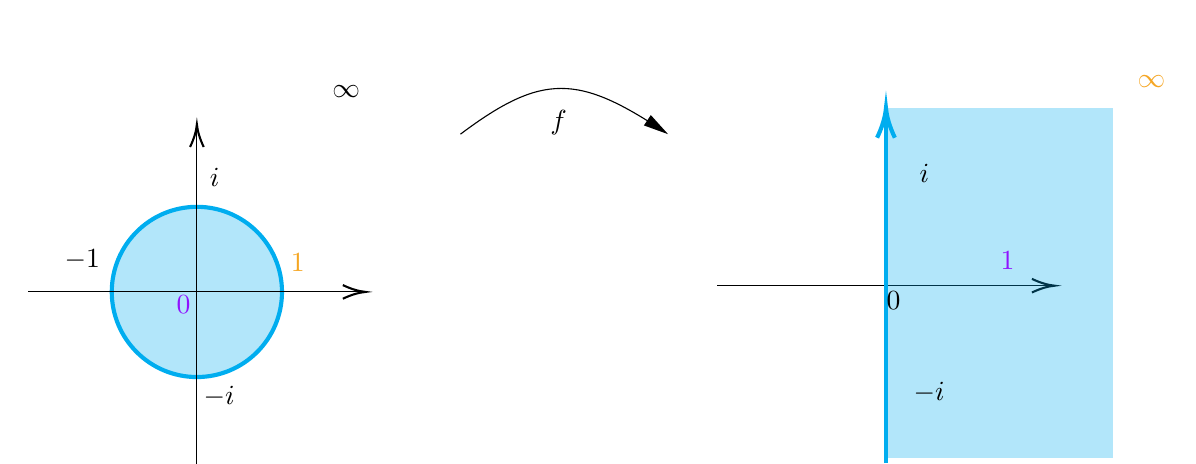
\begin{tikzpicture}[x=0.75pt,y=0.75pt,yscale=-1,xscale=1]
%uncomment if require: \path (0,300); %set diagram left start at 0, and has height of 300

%Shape: Circle [id:dp46487660565461075] 
\draw  [color=cyan  ,draw opacity=1 ][fill=cyan  ,fill opacity=0.3 ][line width=1.5]  (96,156.01) .. controls (96,133.37) and (114.36,115.01) .. (137.01,115.01) .. controls (159.65,115.01) and (178.01,133.37) .. (178.01,156.01) .. controls (178.01,178.66) and (159.65,197.02) .. (137.01,197.02) .. controls (114.36,197.02) and (96,178.66) .. (96,156.01) -- cycle ;
%Curve Lines [id:da6037660096213038] 
\draw    (264,80) .. controls (303.6,50.3) and (320.91,51.23) .. (362.73,79.15) ;
\draw [shift={(364,80)}, rotate = 213.92] [fill=black  ][line width=0.08]  [draw opacity=0] (12,-3) -- (0,0) -- (12,3) -- cycle    ;
%Straight Lines [id:da30485423184171] 
\draw    (55.75,156.01) -- (216.26,156.01) ;
\draw [shift={(218.26,156.01)}, rotate = 180] [color=black  ][line width=0.75]    (10.93,-3.29) .. controls (6.95,-1.4) and (3.31,-0.3) .. (0,0) .. controls (3.31,0.3) and (6.95,1.4) .. (10.93,3.29)   ;
%Straight Lines [id:da03496103337291223] 
\draw    (387.75,153.01) -- (548.26,153.01) ;
\draw [shift={(550.26,153.01)}, rotate = 180] [color=black  ][line width=0.75]    (10.93,-3.29) .. controls (6.95,-1.4) and (3.31,-0.3) .. (0,0) .. controls (3.31,0.3) and (6.95,1.4) .. (10.93,3.29)   ;
%Straight Lines [id:da11880027193931353] 
\draw    (137.01,246.26) -- (137.01,77.26) ;
\draw [shift={(137.01,75.26)}, rotate = 90] [color=black  ][line width=0.75]    (10.93,-3.29) .. controls (6.95,-1.4) and (3.31,-0.3) .. (0,0) .. controls (3.31,0.3) and (6.95,1.4) .. (10.93,3.29)   ;
%Straight Lines [id:da4256972022746721] 
\draw [color=cyan  ,draw opacity=1 ][line width=1.5]    (469.01,238.51) -- (469.01,70.51) ;
\draw [shift={(469.01,67.51)}, rotate = 90] [color=cyan  ,draw opacity=1 ][line width=1.5]    (14.21,-4.28) .. controls (9.04,-1.82) and (4.3,-0.39) .. (0,0) .. controls (4.3,0.39) and (9.04,1.82) .. (14.21,4.28)   ;
%Shape: Rectangle [id:dp17327106892852906] 
\draw  [draw opacity=0][fill=cyan  ,fill opacity=0.3 ] (469.01,67.51) -- (578.26,67.51) -- (578.26,236.26) -- (469.01,236.26) -- cycle ;

% Text Node
\draw (142,95.4) node [anchor=north west][inner sep=0.75pt]    {$i$};
% Text Node
\draw (181,136.4) node [anchor=north west][inner sep=0.75pt]  [color={rgb, 255:red, 245; green, 166; blue, 35 }  ,opacity=1 ]  {$1$};
% Text Node
\draw (139.01,200.42) node [anchor=north west][inner sep=0.75pt]    {$-i$};
% Text Node
\draw (72,134.4) node [anchor=north west][inner sep=0.75pt]    {$-1$};
% Text Node
\draw (126,156.4) node [anchor=north west][inner sep=0.75pt]  [color={rgb, 255:red, 144; green, 19; blue, 254 }  ,opacity=1 ]  {$0$};
% Text Node
\draw (484,93.4) node [anchor=north west][inner sep=0.75pt]    {$i$};
% Text Node
\draw (523,135.4) node [anchor=north west][inner sep=0.75pt]  [color={rgb, 255:red, 144; green, 19; blue, 254 }  ,opacity=1 ]  {$1$};
% Text Node
\draw (481.01,198.42) node [anchor=north west][inner sep=0.75pt]    {$-i$};
% Text Node
\draw (468,154.4) node [anchor=north west][inner sep=0.75pt]    {$0$};
% Text Node
\draw (201,55.4) node [anchor=north west][inner sep=0.75pt]    {$\infty $};
% Text Node
\draw (306,67.4) node [anchor=north west][inner sep=0.75pt]    {$f$};
% Text Node
\draw (589,50.4) node [anchor=north west][inner sep=0.75pt]    {$\textcolor[rgb]{0.96,0.65,0.14}{\infty }$};


\end{tikzpicture}

\section{Recall: infinite series}
\defn $\sum_{n=1}^{\infty}a_n$ converges to $S$ if $\lim_{N\to \infty}S_N=S$ where $S_N=a_1+\dots+a_N$.\sidenote{$S_N$ is the $N$-th partial sum.}

\subsection{Divergence test}
\defn[Divergence test]A pair of contrapositives:\sidenote{Note it's not an \ifnif !}\begin{enumerate}
    \item If $\sum_{n=1}^{\infty}a_n$ converges, then $\lim_{n\to\infty}a_n=0$.
    \item If $\lim_{n\to\infty}a_n\neq 0$ (\textit{including the case where the limit doesn't exist}) then $\sum_{n=1}^{\infty}a_n$ diverges.
\end{enumerate}
\noneg The harmonic series $\sum_{n=1}^{\infty}\frac{1}{n}=1+\frac{1}{2}+\dots$ diverges\sidenote{diverges, but really \textbf{slowly}!} even though $a_n=\frac{1}{n}$ tends to 0 when $n$ tends to $\infty$.

\begin{theorem}
    If $\sum_{n=1}^{\infty}a_n$ converges, then $\lim_{N\to \infty}\sum_{n=N}^{\infty}a_n=\lim_{N\to \infty}S-S_N=0$.\sidenote{In other words, the tail of a convergent series goes to 0.}
\end{theorem}

\begin{theorem}[Cauchy Criterion]
    $\sum_{n=1}^{\infty}a_n$ converges \ifnif for all $\varepsilon>0$, there exists $N\in \N$ such that $k>j>N$ implies $\displaystyle \left|\sum_{n=j-1}^{k}a_n \right|=S_k-S_j<\varepsilon$.
\end{theorem}

\subsection{Integral test}

\defn[Integral test] Define $a_n=f(n)$ for $n\in \N$, where $f:[1,\infty[ \to \R$ is (piecewise) continuous, positive and decreasing. Then $\int_{1}^{\infty}f(x)\, \d x$ converges \ifnif $\sum_{n=1}^{\infty}a_n$ converges.\sidenote{do an improper integral!}

Moreover, $\int_{1}^{N}f(x)\,\d x\leq a_1+\dots+a_N\leq a_1+\int_{1}^{N}f(x)\,\d x$.

\eg Apply the above with $f(x)=\frac{1}{x}$.\sidenote{$a_n=\frac{1}{n}$} Then \begin{align*}
    \ln N\leq 1+\frac{1}{2}+\dots+\frac{1}{N}\leq 1+\ln N
\end{align*}
It is bounded below by a divergent function, so it must be divergent!

\begin{theorem}
    The ``$p$-series'' $\sum_{n=1}^{\infty}\frac{1}{n^p}$ converges \ifnif $p>1$.
\end{theorem}

\defn[Riemann zeta function] \begin{align*}
    \zeta(s)&=\sum_{n=1}^{\infty}\frac{1}{n^s} && \text{for Re}(s)>1
\end{align*}
\rmk Euler figured out: \begin{align*}
    \zeta(2)&=\frac{\pi^2}{6}\\
    \zeta(4)&=\frac{\pi^4}{90}\\
    \zeta(6)&=\frac{\pi^6}{945}\\
    \vdots
\end{align*}
\rmk R. Apéry showed that $\zeta(3)$ is irrational (1979)\sidenote{still an open question in mathematics}:
\[\zeta(3)=\sum_{n=1}^{\infty}\frac{1}{n^3}=1.202\dots\]
but no explicit formula known!

\subsection{Absolute convergence}

\defn A series $\sum_{n=1}^{\infty}a_n$ is:\begin{enumerate}
    \item \textbf{absolutely convergent} if $\sum_{n=1}^{\infty}|a_n|$ converges.\sidenote{Good}
    \item \textbf{conditionally convergent} if $\sum_{n=1}^{\infty}a_n$ converges but $\sum_{n=1}^{\infty}|a_n|$ diverges.\sidenote{BAD}
\end{enumerate}

\begin{theorem}
    Every absolutely convergent series converges.
\end{theorem}
\eg The alternating harmonic series\sidenote{Don't re-parenthesize the terms -- grouping would change the sequence and thus the partial sums!} $$\sum_{n=1}^{\infty}\frac{(-1)^{n+1}}{n}=1-\frac{1}{2}+\frac{1}{3}-\frac{1}{4}+\dots$$ converges to $\ln 2$. But the convergence is conditional because the absolute value $$\sum_{n=1}^{\infty}\left|\frac{(-1)^{n+1}}{n}\right|=\sum_{n=1}^{\infty}\frac{1}{n}$$ does not converge.

\begin{theorem}
    An absolutely convergent series may be rearranged without changing its value. That is, if $\phi:\N\to \N$ is a bijection, then\sidenote{This seems obvious for finite series, but consider how this is extraordinary for infinite series!} $$\sum_{n=1}^{\infty}a_n=\sum_{n=1}^{\infty}a_{\phi(n)}$$
\end{theorem}

\addlink{Riemann Rearrangement Theorem}
\begin{theorem}[Riemann Rearrangement Theorem]
    If $\sum_{n=1}^{\infty}a_n$ is a \uline{conditionally convergent} series of real numbers, then for \textbf{any} $S\in \R\cup \{-\infty,\infty\}$, there is a bijection $\phi:\N\to\N$ such that $\sum_{n=1}^{\infty}a_{\phi(n)}=S$.\sidenote{Meaning we can get it to be equal to whatever we want just by rearranging!}
\end{theorem}

\spl

Now if $\sum_{n=0}^{\infty}a_n$ and $\sum_{n=0}^{\infty}b_n$ converge, one might expect that \begin{align*}
    \left(\sum_{i=0}^{\infty}a_i\right)\left(\sum_{j=0}^{\infty}b_j\right)&=(a_0+a_1+\dots)(b_0+b_1+\dots)\\
    &= a_0b_0+(a_0b_1+a_1b_0)+\dots\\
    &= \sum_{n=0}^{\infty}c_n \text{ where } c_n=\sum_{k=0}^{n}a_kb_{n-k}
\end{align*}
But this only works if both series are absolutely convergent, in which case the new series is absolutely convergent.\sidenote{conditionally convergent doesn't work! See \href{https://stephangarcia.sites.pomona.edu/teaching/24S-135/Lecture/24S-135-Lecture06.pdf}{notes}.}

\subsection{Uniform convergence}
\defn A sequence of functions $f_n: X\to \C$ where $X\subseteq \C$ \textbf{converges uniformly} to $f:X\to \C$ if for all $\varepsilon>0$, there exists a $N\in \N$ such that $n\geq N$ implies $|f_n(z)-f(z)|<\varepsilon$ for all $z\in X$.\sidenote{This is MATH131!}
\drawing{0.6\linewidth}{image-5.png}

\addlink{Uniform convergence preserves continuity}
\begin{theorem}
    If $f_n: X\to \C$ are continuous and converges uniformly on $X$ to $f:X\to\C$, then $f$ is continuous on $X$.\sidenote{unif. conv. preserves continuity}
    In other words, the uniform limit of continuous functions is continuous.
\end{theorem}

\rmk $f_n$ converges to $f$ pointwise on $X$ if $\lim_{n\to \infty}f_n(z)=f(z)$ for all $z\in X$.\sidenote{This doesn't say anything about the rate each point converges.}
\drawing{0.6\linewidth}{image-6.png}

\addlink{Integrals work with uniform convergence}
\begin{theorem}
    If $f_n:[a,b]\to \C$ are continuous and converge uniformly on $[a,b]$ to $f$, then\sidenote{Integrals work with uniform convergence} $$
    \lim_{n\to \infty}\int_{a}^{b}f_n(x)\,\d x = \int_{a}^{b}f(x)\,\d x
    $$
\end{theorem}

\rmk Uniform convergence doesn't necessarily preserve differentiability, limit or derivatives!

\eg $f_n(x)=\sqrt{x^2+\frac{1}{n}}$ on $[-1,1]$ converges uniformly to $f_n(x)=|x|$. But the limit function is \textbf{not} differentiable at $x=0$ even though every $f_n$ were.

\begin{theorem}[Weierstrass $M$-Test] 
    Let $f_n:X\to \C$ satisfy $|f_n(z)|\leq M_n$ for all $z\in X$ and $n\in \N$. If $\sum_{n=1}^{\infty}M_n$ converges, then $\sum_{n=1}^{\infty}f_n(z)$ converges both \textbf{absolutely} and \textbf{uniformly} on $X$.
\end{theorem}

\section{Power series}
\defn A \textbf{power series} is a series of the form $\sum_{n=0}^{\infty}a_n(z-z_0)^n$. The $a_n$ is the \textit{coefficient} and $z_0$ is the \textit{center}.

\subsection{Convergence of geometric series}

\begin{theorem}
    The \textit{geometric series} ($a_n=1, z_0=0$) $\sum_{n=0}^{\infty}z^n$ converges absolutely to $\frac{1}{1-z}$ if $|z|<1$, and it diverges otherwise. 

    Moreover, for each $r\in [0,1[$, the convergence is \textbf{uniform} on $|z|\leq r$.
\end{theorem}
\begin{proof}
    If $|z|\geq 1$, then $z^n\not\to 0$, so by the test of divergence, the series diverges.

    Now suppose $|z|<1$. Then\sidenote{The fact that we can find a formula for this sum is quite rare! } \begin{align*}
        \sum_{n=0}^{\infty}z^n &= \lim_{N\to \infty}\sum_{n=0}^{N-1}z^n\\
        &= \lim_{N\to \infty}(1+z+z^2+\dots+z^{N-1})\\
        &= \lim_{N\to \infty}\frac{1-z^N}{1-z}\\
        &= \frac{1}{1-z} &\text{since }|z|<1
    \end{align*}
    Which gives us point-wise convergence. Then, for any $r$ such that $|z|\leq r<1$, we have \begin{align*}
        \sum_{n=0}^{\infty}|z^n|\leq \sum_{n=0}^{\infty}r^n =\frac{1}{1-r}<\infty
    \end{align*}
    Hence, by the Weierstrass $M$-test, the series converges \textit{absolutely and uniformly} on $|z|\leq r$.
\end{proof}

\rmk Moral of the story: \begin{itemize}
    \item The \textit{radius of convergence} $R=1$ has the property that the series converges on $|z|<R$, and diverges if $|z|>R$.
    
    \item The series converges \textit{uniformly} on $|z|\leq r<1$ but not on $|z|<1$ itself. Why?
    
    Let $r=1$; we need be able to get $N\in \N$ such that for all $n\geq N$, we have $\left|\frac{1-z^N}{1-z}-\frac{1}{1-z}\right|<1$ for all $|z|<1$. However, this is not gonna work: as $z\to 1$, observe that this is going to eventually exceed 1. 

    \item The limit function $\displaystyle \frac{1}{1-z}$ is \textbf{analytic} on $\C\backslash\{1\}$\sidenote{the limit function is well-defined way beyond the $\mathbb{D}$!}. But the geometric series represents this function \underline{only} on $|z|<1$. In a smaller set, the power series represents the function that might originally be defined on a much larger set. The limit function is the \textit{analytic continuation} of the series.
    
    \item The limit function $\displaystyle \frac{1}{1-z}$ is cool if $z\neq 1$\sidenote{in the complex number sense!}, but as long as $|z|=1$ (\textbf{even} if $z\neq 1$), the geometric series diverges!
\end{itemize}

\subsection{Radius of convergence}
\defn The \textbf{limit superior} ($\limsup$) of a sequence of nonnegative real numbers $x_n$ is the largest \textit{limit point}\sidenote{limits of a subsequence of $x_n$} of the $x_n$: $$\limsup_{n\to \infty}x_n=\inf_{n\geq 0}\sup_{m\geq n}x_m$$\sidenote{the RHS as in real analysis}\addlink{Limit superior}
If the sequence is unbounded, the $\limsup$ would be $\infty$.

\eg If $x_n$ is the sequence $0,1,0,1,\dots$ then $\displaystyle\limsup_{n\to \infty}x_n=1$.

\eg If $x_n$ is the sequence $0,1,0,\frac{1}{2}, 0, \frac{1}{3},\dots$, then $\displaystyle\limsup_{n\to \infty}x_n=0$.

\rmk If $x_n$ are nonnegative, then \begin{itemize}
    \item $\displaystyle \limsup_{n\to \infty}(a_n+b_n)=\limsup_{n\to \infty}a_n+\limsup_{n\to \infty}b_n$
    \item $\displaystyle \limsup_{n\to \infty}(a_nb_n)\leq (\limsup_{n\to \infty}a_n)(\limsup_{n\to \infty}b_n)$
\end{itemize}

\addlink{Cauchy-Hadamard formula}
\begin{theorem}[Cauchy-Hadamard]
    Let $\sum_{n=0}^{\infty}a_n(z-z_0)^n$ be a power series. Define $R\in [0,\infty]$ by \sidenote{interpret $\frac{1}{0}=\infty$}\begin{align*}
        \frac{1}{R}=\limsup_{n\to \infty}\sqrt[n]{|a_n|}
    \end{align*}
    Then the $R$ is the \textit{radius of convergence}.
    \begin{enumerate}[label=(\alph*)]
        \item On $|z-z_0|<R$, the series converges \textbf{absolutely}.\sidenote{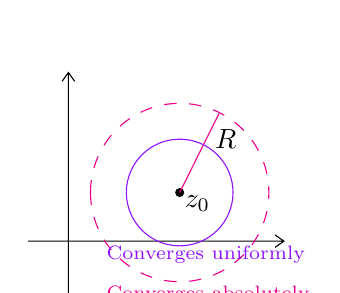
\begin{tikzpicture}[x=0.75pt,y=0.75pt,yscale=-0.6,xscale=.6]
            %uncomment if require: \path (0,300); %set diagram left start at 0, and has height of 300
            
            %Shape: Axis 2D [id:dp5858755410080565] 
            \draw  (50,212.68) -- (255.26,212.68)(82.26,77.28) -- (82.26,267.03) (248.26,207.68) -- (255.26,212.68) -- (248.26,217.68) (77.26,84.28) -- (82.26,77.28) -- (87.26,84.28)  ;
            %Shape: Circle [id:dp24544423482988642] 
            \draw  [color=magenta  ,draw opacity=1 ][dash pattern={on 4.5pt off 4.5pt}] (100,173.64) .. controls (100,134.09) and (132.06,102.03) .. (171.61,102.03) .. controls (211.17,102.03) and (243.23,134.09) .. (243.23,173.64) .. controls (243.23,213.19) and (211.17,245.26) .. (171.61,245.26) .. controls (132.06,245.26) and (100,213.19) .. (100,173.64) -- cycle ;
            %Shape: Circle [id:dp09425242443966897] 
            \draw  [fill=black  ,fill opacity=1 ] (168.46,173.64) .. controls (168.46,171.9) and (169.87,170.48) .. (171.61,170.48) .. controls (173.36,170.48) and (174.77,171.9) .. (174.77,173.64) .. controls (174.77,175.39) and (173.36,176.8) .. (171.61,176.8) .. controls (169.87,176.8) and (168.46,175.39) .. (168.46,173.64) -- cycle ;
            %Straight Lines [id:da3698233641764985] 
            \draw [color=magenta  ,draw opacity=1 ]   (203.26,110.07) -- (171.61,173.64) ;
            %Shape: Circle [id:dp40259923856296376] 
            \draw  [color={rgb, 255:red, 144; green, 19; blue, 254 }  ,draw opacity=1 ] (128.79,173.64) .. controls (128.79,149.99) and (147.96,130.81) .. (171.61,130.81) .. controls (195.27,130.81) and (214.44,149.99) .. (214.44,173.64) .. controls (214.44,197.29) and (195.27,216.47) .. (171.61,216.47) .. controls (147.96,216.47) and (128.79,197.29) .. (128.79,173.64) -- cycle ;
            
            % Text Node
            \draw (198,120.82) node [anchor=north west][inner sep=0.75pt]    {$R$};
            % Text Node
            \draw (173.61,173.88) node [anchor=north west][inner sep=0.75pt]    {$z_{0}$};
            % Text Node
            \draw (110.8,246.42) node [anchor=north west][inner sep=0.75pt]  [color=magenta  ,opacity=1 ] [align=left] {{\scriptsize Converges absolutely}};
            % Text Node
            \draw (110.8,214.62) node [anchor=north west][inner sep=0.75pt]   [align=left] {{\scriptsize \textcolor[rgb]{0.56,0.07,1}{Converges uniformly}}};
            
            
            \end{tikzpicture}} 
            For each $r\in [0,R[$, the convergence is \textbf{uniform} on $|z-z_0|\leq r$.        
        \item If $|z-z_0|>R$ then the series diverges. \rt{For $|z-z_0|=R$ anything could happen!}
    \end{enumerate}
\end{theorem}

\eg We claim that $\exp(z)=\sum_{n=0}^{\infty}\frac{z^n}{n!}$ has an infinite radius of convergence $R=\infty$. To check:
\begin{align*}
    \sqrt[n]{|a_n|} =\sqrt[n]{\frac{1}{n!}} = \frac{1}{\sqrt[n]{n!}}\to 0
\end{align*}
This is because $\sqrt[n]{n!} = \sqrt[n]{1\cdot 2\cdot\dots \cdot n}$, and in $n!$, there are at least $\frac{1}{2}$ terms that are $>\frac{n}{2}$. Thus, $\sqrt[n]{n!}\geq \left(\left(\frac{n}{2}\right)^{\frac{n}{2}}\right)^{\frac{1}{n}}=\left(\frac{n}{2}\right)^{1/2}\to \infty$.

So $R=\infty$ and we are done \begin{tikzpicture}[x=0.75pt,y=0.75pt,yscale=-.2,xscale=.2]%Shape: Smiley Face [id:dp9495597583093132] 
    \draw   (80,136) .. controls (80,116.67) and (95.67,101) .. (115,101) .. controls (134.33,101) and (150,116.67) .. (150,136) .. controls (150,155.33) and (134.33,171) .. (115,171) .. controls (95.67,171) and (80,155.33) .. (80,136) -- cycle ; \draw   (99.6,124.1) .. controls (99.6,122.17) and (101.17,120.6) .. (103.1,120.6) .. controls (105.03,120.6) and (106.6,122.17) .. (106.6,124.1) .. controls (106.6,126.03) and (105.03,127.6) .. (103.1,127.6) .. controls (101.17,127.6) and (99.6,126.03) .. (99.6,124.1) -- cycle ; \draw   (123.4,124.1) .. controls (123.4,122.17) and (124.97,120.6) .. (126.9,120.6) .. controls (128.83,120.6) and (130.4,122.17) .. (130.4,124.1) .. controls (130.4,126.03) and (128.83,127.6) .. (126.9,127.6) .. controls (124.97,127.6) and (123.4,126.03) .. (123.4,124.1) -- cycle ; \draw   (97.5,150) .. controls (109.17,159.33) and (120.83,159.33) .. (132.5,150) ;
    \end{tikzpicture}. We have that $\exp(z)$ has absolute convergence on the entire complex plane!

Absolute convergence means that we can multiply term-by-term:
\begin{align*}
    \exp(z)\exp(w) & = \left(\sum_{n=0}^{\infty}\frac{z^n}{n!}\right)\left(\sum_{n=0}^{\infty}\frac{w^n}{n!}\right)\\
    &= \sum_{n=0}^{\infty}\left(\sum_{k=0}^{\infty}\frac{z^k}{k!}\cdot\frac{w^{n-k}}{(n-k)!}\right)\\
    &= \sum_{n=0}^{\infty}\rt{\frac{1}{n!}}\underset{\text{binomial theorem}}{\underbrace{\sum_{k=0}^{\infty}\frac{\rt{n!}}{k!(n-k)!}z^kw^{n-k}}}\\
    &= \sum_{n=0}^{\infty}{\frac{1}{n!}}(z+w)^n\\
    &= \exp(z+w)
\end{align*}

Now define $e=\exp(1)=\sum_{n=0}^{\infty}\frac{1}{n!}$.

\subsection{Term-by-term differentiation of power series}

\begin{lemma}
    $n^{\frac{1}{n}}\to 1$
\end{lemma}
\begin{proof}[Proof 1] $e^{\log (n^{\frac{1}{n}})}=e^{\frac{\log n}{n}}\to e^{0}=1$ by l'Hopital. So $n^{\frac{1}{n}}\to 1$.
\end{proof}
\begin{proof}[Proof 2 (better)] Write $n^{\frac{1}{n}}=1+\delta_n$ where $\delta_n\geq 0$. The binomial theorem says:
\begin{align*}
    n&= (1+\delta_n)^n\\
    &= \sum_{k=0}^{\infty}{n\choose k}\delta_n^k\cdot 1^{n-k}\\
    &= 1+n\delta_n+\frac{n(n-1)}{2}\delta_n^2+\dots\\
    &\geq 1+\frac{n(n-1)}{2}\delta_n^2
\end{align*}
    Therefore, $n-1\geq \frac{n(n-1)}{2}\delta_n^2$ and we get $\frac{2}{n}\geq \delta_n^2\geq 0$ hence $\delta_n\to 0$.

    Hence $n^{\frac{1}{n}}\to 1$.
\end{proof}

\addlink{Derivative series have the same radius of convergence}
\begin{theorem}
    If $f(z)=\sum_{n=0}^{\infty}a_n(z-z_0)^{n}$ has radius of convergence $R$, then \[f'(z)=\sum_{n=0}^{\infty}na_n(z-z_0)^{n-1}\] for $|z-z_0|<R$. Moreover, the new series also has a radius of convergence $R$.
\end{theorem}
\begin{proof}
    WLOG $R>0$ and $z_0=0$\sidenote{we just translate it; also $R=0$ isn't that meaningful}. 
    
    For $|z|<R$ we write:\sidenote{just splitting the function into two parts}
    \[f(z)=\underset{S_N(z)}{\underbrace{\sum_{n=0}^{N-1}a_nz^n}} + \underset{R_N(z)}{\underbrace{ \sum_{n=N}^{\infty}a_nz^n}}\]
    and the `new series'\[g(z)=\sum_{n=0}^{\infty}na_nz^{n-1}=\lim_{N\to \infty}S'_N(z)\]

    We first prove that the radius of convergence for $g$ is the same as $f$. By Cauchy-Hadamard:
    \begin{align*}
        \frac{1}{R_g}&=\limsup_{n\to \infty}\sqrt[n]{n|a_n|}\\
        &=\limsup_{n\to \infty}(n^{\frac{1}{n}})\sqrt[n]{|a_n|} & \text{by the previous lemma,}\\
        &= \limsup_{n\to \infty}\sqrt[n]{|a_n|}\\
        &= \frac{1}{R}
    \end{align*}
    Thus, $R_g=R$ by Cauchy-Hadamard.

    Next, we need to show that $f'=g$ with $|z|<R$.

    Fix $0\leq |w|<R$ and $\varepsilon>0$. We want a $\delta>0$ such that whenever $|z-w|<\delta$,  we have $\left|\frac{f(z)-f(w)}{z-w}-g(w)\right|<\varepsilon$.\sidenote{just saying that the derivative at any $w$ gets close to $g(w)$}

    We rewrite:\begin{align*}
        \left|\frac{f(z)-f(w)}{z-w}-g(w)\right|
        &= \left| \frac{
            [S_N(z)+R_N(z)]-[S_N(w)+R_N(w)]
        }
        {z-w}
        -g(w)\right|\\
        &= \left|
            \frac{S_N(z)-S_N(w)}{z-w} +
            \frac{R_N(z)-R_N(w)}{z-w} +
            \gt{S'_N(w)-S'_N(w)} -
            g(w)
            \right|\\
        &\leq \left| S'_N(w)-g(w)
            \right| + 
            \left| \frac{R_N(z)-R_N(w)}{z-w}
            \right| + 
            \left| \frac{S_N(z)-S_N(w)}{z-w} - S'_N(w)
            \right|
    \end{align*}

    \begin{itemize}
        \item \textbf{1st term}: by def of $g$ and $g(z)=\lim_{N\to \infty}S'_N(z)$, we can always find some $N_1\in \N$ such that any $N\geq N_1$ gives us $\left| S'_N(w)-g(w)\right| <\frac{\varepsilon}{3} $.
        \item \textbf{2nd term}: since $|w|<R$, there is an $r$ such that $|w|<r<R$.\sidenote{work on a smaller disk}
        
        For $|z|<r$, we have \begin{align*}
            \left| \frac{R_N(z)-R_N(w)}{z-w}
            \right| &= \frac{1}{|z-w|}\left|\sum_{n=N}^{\infty}a_nz^n= - \sum_{n=N}^{\infty} a_nw^n\right|\\
            &\leq \sum_{n=N}^{\infty} |a_n| \left|\frac{z^n-w^n}{z-w}\right|\\
            &= \sum_{n=N}^{\infty} |a_n| \left|\frac{z^n}{z}\cdot \frac{1-\frac{w^n}{z^n}}{1-\frac{w}{z}}\right| & \text{by geometric sequence}\\
            &= \sum_{n=N}^{\infty} |a_n| \left|\frac{z^n}{z}\cdot \left(
                1+\left(\frac{w}{z}\right) + \left(\frac{w}{z}\right)^2 + \dots + \left(\frac{w}{z}\right)^{n-1}
            \right)\right|\\
            &= \sum_{n=N}^{\infty} |a_n| \left|
                z^{n-1}+z^{n-2}w+\dots + zw^{n-2}+w^{n-1}
            \right|\\
            &\leq \sum_{n=N}^{\infty} |a_n|\cdot n\cdot r^{n-1} \text{by }|z|,|w|<r<R
        \end{align*}
        Thus, there exists an $N_2\in \N$ such that any $N\geq N_2$ gives us $$\left| \frac{R_N(z)-R_N(w)}{z-w}
        \right|<\frac{\varepsilon}{3}$$
        \item \textbf{3rd term}: let $N=\max\{N_1,N_2\}$. The definition\sidenote{review def of derivatives!} of $S'_N(w)$ provides $\gamma>0$ such that if $|z-w|<\gamma$, then we have $\left| \frac{S_N(z)-S_N(w)}{z-w} - S'_N(w)
        \right|<\frac{\varepsilon}{3}$.
    \end{itemize}

    Now if $0<\delta<\min\{\gamma, r-|w|\}$, then the 3 terms above are all $<\frac{\varepsilon}{3}$. Hence, $\left|\frac{f(z)-f(w)}{z-w}-g(w)\right|<\varepsilon$ holds for this $\delta$.
\end{proof}

\addlink{Power series are infinitely differentiable}
\begin{corollary}
    A power series $f(z)=\sum_{n=0}^{\infty}a_n(z-z_0)^n$ with $R>0$ is \dashuline{infinitely differentiable} on $|z-z_0|<R$. Moreover, \[a_n = \frac{f^{(n)}(z_0)}{n!}\] are the coefficients of the terms of the power series. \sidenote{prove by keep taking derivatives!}
\end{corollary}

\addlink{Power series expansions are unique}
\begin{corollary}
    Power series expansions are unique.\sidenote{because there is a unique formula for coeffs.} That is, if $r>0$ and \[\sum_{n=0}^{\infty}a_n(z-z_0)^{n} = \sum_{n=0}^{\infty}b_n(z-z_0)^{n}\]
    on $|z-z_0|<r$, then $a_n=b_n$ for $n\geq 0$.
\end{corollary}

\rmk Recall that $\exp(z)=\sum_{n=0}^{\infty}\frac{z^n}{n!}$ has a radius of convergence $\infty$ (it's an \textit{entire} function). Now, if we differentiate it term-by-term:
\begin{align*}
    \frac{\d}{\d z}\exp(z)&=\frac{\d}{\d z}\sum_{n=0}^{\infty}\frac{z^n}{n!}\\
    &= \sum_{n=0}^{\infty}\frac{z^{n-1}}{(n-1)!} &\text{let }k=n-1\\
    &= \sum_{k=0}^{\infty} \frac{z^k}{k!}\\
    &= \exp(z)
\end{align*}
Thus, the derivative of $\exp(z)$ is itself! Moreover, $\exp(1)=\sum_{n=0}^{\infty}\frac{1}{n!}=e$.

\rmk We claim that $\exp(z)=e^z$.

Since $e^ze^{c-z}$ is a constant for all constant $c,z$, we have \[\frac{\d}{\d z}(e^ze^{c-z})=0\]
to recover the constant $e^ze^{c-z}$, we let $z=0$, giving us \[e^{z}e^{c-z}=e^{c}\]
which is the addition formula!

Therefore, \begin{align*}
    \exp(n) &= \exp(1+1+\dots+1)\\
    &= exp(1)^{n}\\
    &=e^n
\end{align*}

\section{Elementary functions}

Now that we have derived $e$, we could use it to derive $\sin$ and $\cos$:

\addlink{Trig functions in terms of \textit{e}}
\defn \begin{align*}
    \cos(z) &= \frac{e^{iz}+e^{-iz}}{2}\\
    &= \sum_{n=0}^{\infty}\frac{(-1)^nz^{2n}}{(2n)!}
\end{align*}
\begin{align*}
    \sin(z) &= \frac{e^{iz}-e^{-iz}}{2i}\\
    &= \sum_{n=0}^{\infty}\frac{(-1)^nz^{2n+1}}{(2n+1)!}
\end{align*}
We observe that we have the following property:
\begin{itemize}
    \item Radius of convergence $R=\infty$
    \item $(\cos z)'=-\sin z, (\sin z)'=\cos z$
    \item $\cos x= \mathrm{Re~}(e^{ix}), \sin x = \mathrm{Im~} e^{ix}$ for all $x\in \R$
    \item $\cos (-z)=\cos z, \sin(-z)=-\sin z$
    \item $\cosh x = \frac{e^x+e^{-x}}{2}$ so $\cosh (ix)=\cos x$
    \item $e^{iz}=\cos z+i\sin z$
    \item \begin{align*}
        \cos^2z+\sin^2z &= \left(\frac{e^{iz}+e^{-iz}}{2}\right)^2 + \left(\frac{e^{iz}-e^{-iz}}{2i}\right)^2\\
        &= \frac{1}{4}(e^{2iz}+2+e^{-2iz})-\frac{1}{4}(e^{2iz}-2+e^{-2iz})\\
        &= 1\qquad \forall z\in \C
    \end{align*}
    \item \begin{align*}
        \cos^2z &= \left(\frac{e^{iz}+e^{-iz}}{2}\right)^2\\
        &= \frac{1}{4}(e^{2iz}+2+e^{-2iz})\\
        &= \frac{1}{2} + \frac{e^{2iz}+e^{-2iz}}{4}\\
        &= \frac{1}{2}(1+\cos 2z)
    \end{align*}
    \item If $x\in \R$ then $\cos x, \sin x$ are real. We get $|\sin x|,|\cos x|\leq 1$.
\end{itemize}

\addlink{Periodicity of functions}
\defn $f:\C\to\C$ is \textbf{periodic} with a \textit{period} $\omega$ if $f(z+\omega)=f(z)$ for all $z\in \C$.

\addlink{Definition of π}
\begin{theorem}
    There exists a positive real number $\pi$ such that:\begin{enumerate}[label=(\alph *)]
        \item $\cos z, \sin z$ have period $2\pi$
        \item $e^z$ is periodic with period $2\pi i$
        \item $\pi$ is the area of the unit circle
    \end{enumerate}
\end{theorem}

\begin{proof}
    By Euler's formula, it suffices to consider $e^{iz}$ only. If $\omega$ is a period of $e^{iz}$, then \[e^{iz}=e^{i(z+\omega)}=e^{iz}e^{i\omega}\] which only happens if $e^{i\omega}=1$. Conversely, if $e^{i\omega}=1$, then $e^{i(z+\omega)}=e^{iz}$.

    Hence, $\omega$ is a period of $e^{iz}$ \ifnif $e^{iw}=1$.
\end{proof}

\proposition $\sin x\leq x$ for all $x\geq 0$.\sidenote{This is the first term in the power series 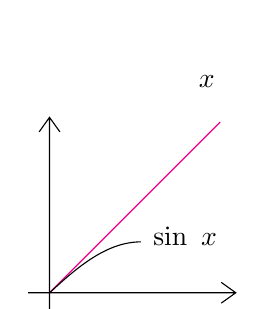
\begin{tikzpicture}[x=0.75pt,y=0.75pt,yscale=-1,xscale=1]
    %uncomment if require: \path (0,300); %set diagram left start at 0, and has height of 300
    
    %Shape: Axis 2D [id:dp008141030370613311] 
    \draw  (50,162.51) -- (150,162.51)(60.26,78) -- (60.26,178) (143,157.51) -- (150,162.51) -- (143,167.51) (55.26,85) -- (60.26,78) -- (65.26,85)  ;
    %Straight Lines [id:da3006663806705201] 
    \draw [color=magenta  ,draw opacity=1 ]   (60.26,162.51) -- (142.51,80.26) ;
    %Shape: Wave [id:dp8304296493911976] 
    \draw   (104.26,138) .. controls (88.39,138) and (74.44,149.34) .. (60.26,162.59) ;
    
    % Text Node
    \draw (131,56.4) node [anchor=north west][inner sep=0.75pt]    {$x$};
    % Text Node
    \draw (109,129.4) node [anchor=north west][inner sep=0.75pt]    {$\sin \ x$};
    
    
    \end{tikzpicture}
    }
\begin{proof}
    Since $|\cos t|\leq 1$, \begin{align*}
        x-\sin x &= (x-\sin x)-(0-\sin 0)\\
        &= \int_{0}^{x}\underset{\geq 0}{\underbrace{1-\cos t}}\d t \qquad \text{by FTC}\\
        &\geq 0
    \end{align*}
\end{proof}

\proposition
In addition, $\cos x\geq 1-\frac{x^2}{2}$ for $x\geq 0$.\sidenote{These are the first 2 terms in the power series

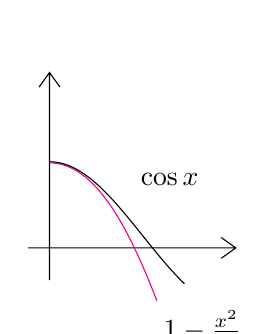
\begin{tikzpicture}[x=0.75pt,y=0.75pt,yscale=-1,xscale=1]
    %uncomment if require: \path (0,300); %set diagram left start at 0, and has height of 300
    
    %Shape: Axis 2D [id:dp008141030370613311] 
    \draw  (50,162.51) -- (150,162.51)(60.26,78) -- (60.26,178) (143,157.51) -- (150,162.51) -- (143,167.51) (55.26,85) -- (60.26,78) -- (65.26,85)  ;
    %Curve Lines [id:da027619260095050446] 
    \draw [color=magenta  ,draw opacity=1 ]   (60.13,121.51) .. controls (82.26,121.51) and (98.26,152.51) .. (112,188) ;
    %Shape: Wave [id:dp87403708438032] 
    \draw   (60.26,121) .. controls (76.54,121) and (90.58,138.44) .. (105.26,156.76) .. controls (111.96,165.13) and (118.54,173.32) .. (125.26,179.74) ;
    
    % Text Node
    \draw (114,191.4) node [anchor=north west][inner sep=0.75pt]    {$1-\frac{x^{2}}{2}$};
    % Text Node
    \draw (103,125.4) node [anchor=north west][inner sep=0.75pt]    {$\cos x$};
    
    
    \end{tikzpicture}
    }
\begin{proof}
    The previous prop gives:
    \begin{align*}
        \cos x -1 &= \cos x -\cos 0\\
        &= \int_{0}^{x}-\sin t\d t\\
        &\geq \int_{0}^{x}- t\d t\\
        &= \frac{-x^2}{2}
    \end{align*}
\end{proof}

\proposition Furthermore, for $x\geq 0$: \begin{itemize}
    \item $\sin x\geq x^3-\frac{x^3}{6}$
    \item $\cos x\leq 1-\frac{x^2}{2}+\frac{x^4}{24}$
\end{itemize}

\begin{proposition}
    There exists $x_0\in (0,\sqrt{3})$ such that $\cos x_0=0$.
   \[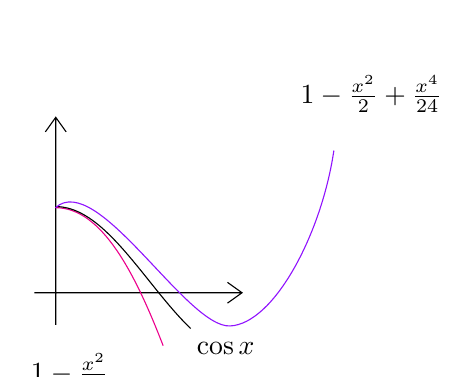
\begin{tikzpicture}[x=0.75pt,y=0.75pt,yscale=-1,xscale=1]
    %uncomment if require: \path (0,300); %set diagram left start at 0, and has height of 300
    
    %Shape: Axis 2D [id:dp008141030370613311] 
    \draw  (50,162.51) -- (150,162.51)(60.26,78) -- (60.26,178) (143,157.51) -- (150,162.51) -- (143,167.51) (55.26,85) -- (60.26,78) -- (65.26,85)  ;
    %Curve Lines [id:da027619260095050446] 
    \draw [color=magenta  ,draw opacity=1 ]   (60.13,121.51) .. controls (82.26,121.51) and (98.26,152.51) .. (112,188) ;
    %Shape: Wave [id:dp87403708438032] 
    \draw   (60.26,121) .. controls (76.54,121) and (90.58,138.44) .. (105.26,156.76) .. controls (111.96,165.13) and (118.54,173.32) .. (125.26,179.74) ;
    %Curve Lines [id:da00092922647570437] 
    \draw [color={rgb, 255:red, 144; green, 19; blue, 254 }  ,draw opacity=1 ]   (60.13,121.51) .. controls (80.26,103.51) and (123.26,179.51) .. (144.26,178.51) .. controls (165.26,177.51) and (188.26,134.51) .. (194.26,94) ;
    
    % Text Node
    \draw (47,190.4) node [anchor=north west][inner sep=0.75pt]    {$1-\frac{x^{2}}{2}$};
    % Text Node
    \draw (127,185.4) node [anchor=north west][inner sep=0.75pt]    {$\cos x$};
    % Text Node
    \draw (177,56.4) node [anchor=north west][inner sep=0.75pt]    {$1-\frac{x^{2}}{2} +\frac{x^{4}}{24}$};
    
    
    \end{tikzpicture}
    \]
\end{proposition}
\begin{proof}
    By the previous prop, we have $\cos \sqrt{3}\leq  1-\frac{\sqrt 3^2}{2}+\frac{\sqrt 3^4}{24}=\frac{1}{8}< 0$. Moreover, $\cos 0=1>0$, by IVT, there exists $x_0\in (0,\sqrt{3})$ such that $\cos x_0=0$.
\end{proof}

\begin{proposition}
    $\omega_0=4x_0$ is a period of $e^{iz}$. 
\end{proposition}
\begin{proof}
    Since $\cos x_0=0$, we have $\sin x_0=\pm 1$. Then $e^{ix_0}=\pm i$. We have $(\pm i)^4=1$, so $e^{4ix_0}=1=e^{0}$, so $\omega_0=4x_0$ is a period of $e^{iz}$.
\end{proof}

\begin{proposition}
    $\omega_0$ is the \textit{smallest} positive period of $e^{iz}$.
\end{proposition}

\begin{proposition}
    All periods of $e^{iz}$ are integer multiples of $2\pi=4x_0$.
\end{proposition}

\begin{proof}
    Define $\pi=2x_0$. The area of unit circle is \begin{align*}
        4\int_{0}^{1}\sqrt{1-x^2}\d x &= 4\int_{0}^{\frac{\pi}{2}}\sqrt{1-\sin^2 \theta}\d \theta\\
        &= 4\int_{0}^{\frac{\pi}{2}}\frac{1}{2}(1+\cos 2\theta)\d \theta\\
        &= \pi
    \end{align*}
\end{proof}

\subsection{Complex logarithm}
We know: $e^0=1,e^1=\sum_{n=0}^{\infty}\frac{1}{n!}=2.718\dots$

Since $\frac{\d}{\d x}e^x=e^x$, it is positive. If $x>0$, we conclude that $e^x$ is strictly increasing! As $e^x=\sum_{n=0}^{\infty}\frac{x^n}{n!}>1+x$, so $\lim_{x\to \infty}e^x=\infty$,

Therefore, $e^x$ is a \textbf{bijection} from $\R$ to $(0,\infty)$. This means it has an inverse that is a bijection from $(0,\infty)$ to $\R$.

\defn $\ln x$ is the inverse of $e^x$ for $x\in (0,+\infty)$.

Now what about the complex case? Let $z\neq 0$ and $z=re^{i\theta}$\sidenote{cf. trig properties} where $r=|z|>0$ and $\theta=\arg z\in \R$.\sidenote{Only determined up to addition of multiples of $2\pi$}

Hence, $z=re^{i\theta}=e^{\ln r}e^{i\theta}=e^{\ln r+i\theta}$. However, the $\theta$ is ambiguous to addition of multiples of $2\pi$!

\addlink{Logarithm}
\defn If $z\neq 0$, a \textbf{logarithm} of $z$ is a $w\in \C$ such that $e^{w}=z$.

We could graph the function $e^z$ with $z\in \C$:       
\[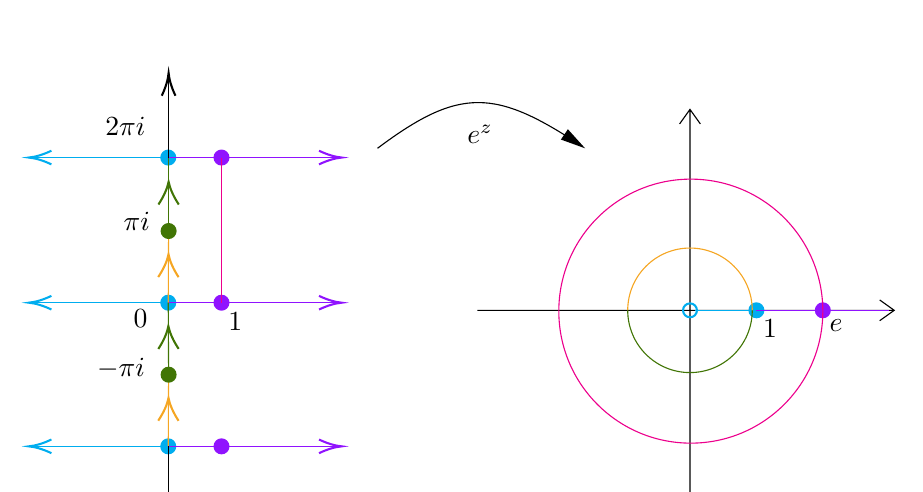
\begin{tikzpicture}[x=0.75pt,y=0.75pt,yscale=-1,xscale=1]
    %uncomment if require: \path (0,300); %set diagram left start at 0, and has height of 300
    
    %Straight Lines [id:da8785590871760756] 
    \draw [color={rgb, 255:red, 144; green, 19; blue, 254 }  ,draw opacity=1 ]   (145.63,130.39) -- (201.55,130.39) ;
    \draw [shift={(203.55,130.39)}, rotate = 180] [color={rgb, 255:red, 144; green, 19; blue, 254 }  ,draw opacity=1 ][line width=0.75]    (10.93,-3.29) .. controls (6.95,-1.4) and (3.31,-0.3) .. (0,0) .. controls (3.31,0.3) and (6.95,1.4) .. (10.93,3.29)   ;
    %Straight Lines [id:da1618236675525775] 
    \draw [color=cyan  ,draw opacity=1 ]   (119.98,130.39) -- (54.75,130.39) ;
    \draw [shift={(52.75,130.39)}, rotate = 360] [color=cyan  ,draw opacity=1 ][line width=0.75]    (10.93,-3.29) .. controls (6.95,-1.4) and (3.31,-0.3) .. (0,0) .. controls (3.31,0.3) and (6.95,1.4) .. (10.93,3.29)   ;
    \draw [shift={(119.98,130.39)}, rotate = 180] [color=cyan  ,draw opacity=1 ][fill=cyan  ,fill opacity=1 ][line width=0.75]      (0, 0) circle [x radius= 3.35, y radius= 3.35]   ;
    %Straight Lines [id:da8267712506988469] 
    \draw [color={rgb, 255:red, 144; green, 19; blue, 254 }  ,draw opacity=1 ]   (119.98,130.39) -- (145.63,130.39) ;
    \draw [shift={(145.63,130.39)}, rotate = 0] [color={rgb, 255:red, 144; green, 19; blue, 254 }  ,draw opacity=1 ][fill={rgb, 255:red, 144; green, 19; blue, 254 }  ,fill opacity=1 ][line width=0.75]      (0, 0) circle [x radius= 3.35, y radius= 3.35]   ;
    %Straight Lines [id:da2374921790479616] 
    \draw [color={rgb, 255:red, 144; green, 19; blue, 254 }  ,draw opacity=1 ]   (145.63,199.6) -- (201.55,199.6) ;
    \draw [shift={(203.55,199.6)}, rotate = 180] [color={rgb, 255:red, 144; green, 19; blue, 254 }  ,draw opacity=1 ][line width=0.75]    (10.93,-3.29) .. controls (6.95,-1.4) and (3.31,-0.3) .. (0,0) .. controls (3.31,0.3) and (6.95,1.4) .. (10.93,3.29)   ;
    %Straight Lines [id:da03468902350963088] 
    \draw [color=cyan  ,draw opacity=1 ]   (119.98,199.6) -- (54.75,199.6) ;
    \draw [shift={(52.75,199.6)}, rotate = 360] [color=cyan  ,draw opacity=1 ][line width=0.75]    (10.93,-3.29) .. controls (6.95,-1.4) and (3.31,-0.3) .. (0,0) .. controls (3.31,0.3) and (6.95,1.4) .. (10.93,3.29)   ;
    \draw [shift={(119.98,199.6)}, rotate = 180] [color=cyan  ,draw opacity=1 ][fill=cyan  ,fill opacity=1 ][line width=0.75]      (0, 0) circle [x radius= 3.35, y radius= 3.35]   ;
    %Straight Lines [id:da3208922622885413] 
    \draw [color={rgb, 255:red, 144; green, 19; blue, 254 }  ,draw opacity=1 ]   (119.98,199.6) -- (145.63,199.6) ;
    \draw [shift={(145.63,199.6)}, rotate = 0] [color={rgb, 255:red, 144; green, 19; blue, 254 }  ,draw opacity=1 ][fill={rgb, 255:red, 144; green, 19; blue, 254 }  ,fill opacity=1 ][line width=0.75]      (0, 0) circle [x radius= 3.35, y radius= 3.35]   ;
    %Straight Lines [id:da4709032693595072] 
    \draw [color={rgb, 255:red, 144; green, 19; blue, 254 }  ,draw opacity=1 ]   (145.63,60.46) -- (201.55,60.46) ;
    \draw [shift={(203.55,60.46)}, rotate = 180] [color={rgb, 255:red, 144; green, 19; blue, 254 }  ,draw opacity=1 ][line width=0.75]    (10.93,-3.29) .. controls (6.95,-1.4) and (3.31,-0.3) .. (0,0) .. controls (3.31,0.3) and (6.95,1.4) .. (10.93,3.29)   ;
    %Straight Lines [id:da05828217640270972] 
    \draw [color=cyan  ,draw opacity=1 ]   (119.98,60.46) -- (54.75,60.46) ;
    \draw [shift={(52.75,60.46)}, rotate = 360] [color=cyan  ,draw opacity=1 ][line width=0.75]    (10.93,-3.29) .. controls (6.95,-1.4) and (3.31,-0.3) .. (0,0) .. controls (3.31,0.3) and (6.95,1.4) .. (10.93,3.29)   ;
    \draw [shift={(119.98,60.46)}, rotate = 180] [color=cyan  ,draw opacity=1 ][fill=cyan  ,fill opacity=1 ][line width=0.75]      (0, 0) circle [x radius= 3.35, y radius= 3.35]   ;
    %Straight Lines [id:da6226539504724369] 
    \draw [color={rgb, 255:red, 144; green, 19; blue, 254 }  ,draw opacity=1 ]   (119.98,60.46) -- (145.63,60.46) ;
    \draw [shift={(145.63,60.46)}, rotate = 0] [color={rgb, 255:red, 144; green, 19; blue, 254 }  ,draw opacity=1 ][fill={rgb, 255:red, 144; green, 19; blue, 254 }  ,fill opacity=1 ][line width=0.75]      (0, 0) circle [x radius= 3.35, y radius= 3.35]   ;
    %Straight Lines [id:da35528692959663144] 
    \draw [color={rgb, 255:red, 245; green, 166; blue, 35 }  ,draw opacity=1 ]   (119.98,130.39) -- (120.15,95.86) ;
    \draw [shift={(120.1,107.13)}, rotate = 90.28] [color={rgb, 255:red, 245; green, 166; blue, 35 }  ,draw opacity=1 ][line width=0.75]    (10.93,-4.9) .. controls (6.95,-2.3) and (3.31,-0.67) .. (0,0) .. controls (3.31,0.67) and (6.95,2.3) .. (10.93,4.9)   ;
    %Straight Lines [id:da8648044267590989] 
    \draw [color={rgb, 255:red, 65; green, 117; blue, 5 }  ,draw opacity=1 ]   (120.15,95.86) -- (120.15,60.46) ;
    \draw [shift={(120.15,72.16)}, rotate = 90] [color={rgb, 255:red, 65; green, 117; blue, 5 }  ,draw opacity=1 ][line width=0.75]    (10.93,-4.9) .. controls (6.95,-2.3) and (3.31,-0.67) .. (0,0) .. controls (3.31,0.67) and (6.95,2.3) .. (10.93,4.9)   ;
    \draw [shift={(120.15,95.86)}, rotate = 270] [color={rgb, 255:red, 65; green, 117; blue, 5 }  ,draw opacity=1 ][fill={rgb, 255:red, 65; green, 117; blue, 5 }  ,fill opacity=1 ][line width=0.75]      (0, 0) circle [x radius= 3.35, y radius= 3.35]   ;
    %Straight Lines [id:da878911184832804] 
    \draw [color={rgb, 255:red, 245; green, 166; blue, 35 }  ,draw opacity=1 ]   (119.98,199.6) -- (120.15,165.07) ;
    \draw [shift={(120.1,176.34)}, rotate = 90.28] [color={rgb, 255:red, 245; green, 166; blue, 35 }  ,draw opacity=1 ][line width=0.75]    (10.93,-4.9) .. controls (6.95,-2.3) and (3.31,-0.67) .. (0,0) .. controls (3.31,0.67) and (6.95,2.3) .. (10.93,4.9)   ;
    %Straight Lines [id:da0013946467543932695] 
    \draw [color={rgb, 255:red, 65; green, 117; blue, 5 }  ,draw opacity=1 ]   (120.15,165.07) -- (119.98,130.39) ;
    \draw [shift={(120.04,141.73)}, rotate = 89.72] [color={rgb, 255:red, 65; green, 117; blue, 5 }  ,draw opacity=1 ][line width=0.75]    (10.93,-4.9) .. controls (6.95,-2.3) and (3.31,-0.67) .. (0,0) .. controls (3.31,0.67) and (6.95,2.3) .. (10.93,4.9)   ;
    \draw [shift={(120.15,165.07)}, rotate = 269.72] [color={rgb, 255:red, 65; green, 117; blue, 5 }  ,draw opacity=1 ][fill={rgb, 255:red, 65; green, 117; blue, 5 }  ,fill opacity=1 ][line width=0.75]      (0, 0) circle [x radius= 3.35, y radius= 3.35]   ;
    %Straight Lines [id:da6431192925230409] 
    \draw    (120.15,60.46) -- (120.15,21.72) ;
    \draw [shift={(120.15,19.72)}, rotate = 90] [color=black  ][line width=0.75]    (10.93,-3.29) .. controls (6.95,-1.4) and (3.31,-0.3) .. (0,0) .. controls (3.31,0.3) and (6.95,1.4) .. (10.93,3.29)   ;
    %Straight Lines [id:da4817110891560017] 
    \draw    (119.98,225.34) -- (119.98,199.6) ;
    %Curve Lines [id:da15130320225307914] 
    \draw    (220.8,56) .. controls (260.4,26.3) and (277.71,27.23) .. (319.53,55.15) ;
    \draw [shift={(320.8,56)}, rotate = 213.92] [fill=black  ][line width=0.08]  [draw opacity=0] (12,-3) -- (0,0) -- (12,3) -- cycle    ;
    %Shape: Axis 2D [id:dp10703039654547442] 
    \draw  (268.95,134.06) -- (469.75,134.06)(371.35,37.26) -- (371.35,229.26) (462.75,129.06) -- (469.75,134.06) -- (462.75,139.06) (366.35,44.26) -- (371.35,37.26) -- (376.35,44.26)  ;
    %Straight Lines [id:da39023709471268675] 
    \draw [color=cyan  ,draw opacity=1 ]   (373.7,134.06) -- (403.35,134.06) ;
    \draw [shift={(403.35,134.06)}, rotate = 0] [color=cyan  ,draw opacity=1 ][fill=cyan  ,fill opacity=1 ][line width=0.75]      (0, 0) circle [x radius= 3.35, y radius= 3.35]   ;
    \draw [shift={(371.35,134.06)}, rotate = 0] [color=cyan  ,draw opacity=1 ][line width=0.75]      (0, 0) circle [x radius= 3.35, y radius= 3.35]   ;
    %Straight Lines [id:da20992201553768708] 
    \draw [color={rgb, 255:red, 144; green, 19; blue, 254 }  ,draw opacity=1 ]   (435.35,134.06) -- (467.35,134.06) ;
    \draw [shift={(435.35,134.06)}, rotate = 0] [color={rgb, 255:red, 144; green, 19; blue, 254 }  ,draw opacity=1 ][fill={rgb, 255:red, 144; green, 19; blue, 254 }  ,fill opacity=1 ][line width=0.75]      (0, 0) circle [x radius= 3.35, y radius= 3.35]   ;
    %Straight Lines [id:da895300882766211] 
    \draw [color={rgb, 255:red, 144; green, 19; blue, 254 }  ,draw opacity=1 ]   (403.35,134.06) -- (435.35,134.06) ;
    %Shape: Arc [id:dp17152249012602994] 
    \draw  [draw opacity=0] (341.35,134.06) .. controls (341.35,134.06) and (341.35,134.06) .. (341.35,134.06) .. controls (341.35,117.49) and (354.78,104.06) .. (371.35,104.06) .. controls (387.92,104.06) and (401.35,117.49) .. (401.35,134.06) .. controls (401.35,134.06) and (401.35,134.06) .. (401.35,134.06) -- (371.35,134.06) -- cycle ; \draw [color={rgb, 255:red, 245; green, 166; blue, 35 }  ,draw opacity=1 ]   (341.35,134.06) .. controls (341.35,117.49) and (354.78,104.06) .. (371.35,104.06) .. controls (387.92,104.06) and (401.35,117.49) .. (401.35,134.06) ;  
    %Shape: Arc [id:dp054572774151422365] 
    \draw  [draw opacity=0] (401.35,134.06) .. controls (401.35,134.06) and (401.35,134.06) .. (401.35,134.06) .. controls (401.35,150.63) and (387.92,164.06) .. (371.35,164.06) .. controls (354.78,164.06) and (341.35,150.63) .. (341.35,134.06) .. controls (341.35,134.06) and (341.35,134.06) .. (341.35,134.06) -- (371.35,134.06) -- cycle ; \draw [color={rgb, 255:red, 65; green, 117; blue, 5 }  ,draw opacity=1 ]   (401.35,134.06) .. controls (401.35,150.63) and (387.92,164.06) .. (371.35,164.06) .. controls (354.78,164.06) and (341.35,150.63) .. (341.35,134.06) ;  
    %Straight Lines [id:da7090062681421083] 
    \draw [color=magenta  ,draw opacity=1 ]   (145.63,60.46) -- (145.63,130.39) ;
    %Shape: Circle [id:dp2705523730959791] 
    \draw  [color=magenta  ,draw opacity=1 ] (308.15,134.46) .. controls (308.15,99.34) and (336.63,70.86) .. (371.75,70.86) .. controls (406.88,70.86) and (435.35,99.34) .. (435.35,134.46) .. controls (435.35,169.59) and (406.88,198.06) .. (371.75,198.06) .. controls (336.63,198.06) and (308.15,169.59) .. (308.15,134.46) -- cycle ;
    
    % Text Node
    \draw (102,132.4) node [anchor=north west][inner sep=0.75pt]    {$0$};
    % Text Node
    \draw (147.63,133.79) node [anchor=north west][inner sep=0.75pt]    {$1$};
    % Text Node
    \draw (88.4,40) node [anchor=north west][inner sep=0.75pt]    {$2\pi i$};
    % Text Node
    \draw (97.2,85.6) node [anchor=north west][inner sep=0.75pt]    {$\pi i$};
    % Text Node
    \draw (84.4,156) node [anchor=north west][inner sep=0.75pt]    {$-\pi i$};
    % Text Node
    \draw (262.8,43.4) node [anchor=north west][inner sep=0.75pt]    {$e^{z}$};
    % Text Node
    \draw (405.35,137.46) node [anchor=north west][inner sep=0.75pt]    {$1$};
    % Text Node
    \draw (437.35,137.46) node [anchor=north west][inner sep=0.75pt]    {$e$};
    
    
    \end{tikzpicture}
    \]

\defn If $\Omega$ is a region in $\C$, then a continuous $l:\Omega \to \C$ is a \textbf{branch} of the logarithm if $e^{l(z)}=z$ for all $z\in \Omega$.\sidenote{note $0\notin \Omega$}

\addlink{Principal branch of the logarithm}
\eg If $\Omega=\C\backslash(-\infty, 0]$ such that $\theta\in (-\pi,\pi)$, a logarithm could be defined on it. This is the \textbf{principal branch} of the logarithm.\sidenote{See \href{https://stephangarcia.sites.pomona.edu/teaching/24S-135/Lecture/24S-135-Lecture10.pdf}{graphed Riemann surface}}

\addlink{First derivative of ln}
\rmk Suppose $l(z)$ is a branch of the logarithm and $l$ is analytic, then: \[e^{l(z)}=z\implies \frac{\d}{\d z}e^{l(z)} = l'(z)e^{l(z)}=1\]

Since $e^{l(z)}=z$, we conclude $l'(z)=\frac{1}{z}$.

\subsection{Complex power}
\defn If $z\neq 0$, \textit{define} $z^{a}=e^{a\log z}$.\sidenote{NOT well-defined!}

\rmk The definition of complex powers should coincide with the old one: $z^n=\underset{n}{\underbrace{z\cdot z\cdot\dots\cdot z}=r^ne^{in\theta}}$.

Check: \begin{align*}
    z^n&=e^{n\log z}=e^{n(\ln r+i\theta+i2\pi k)}\\
    &= e^{n\ln r}e^{in\theta}\underset{=1}{\underbrace{e^{i2\pi nk}}}\\
    &= r^ne^{in\theta}
\end{align*} is true for any $k\in \Z$.

How about $n$-th roots?
\begin{align*}
    z^{\frac{1}{n}} &= e^{\frac{1}{n}\log z}\\
    &= e^{\frac{1}{n}(\ln r+i\theta+i2\pi k)}\\
    &= e^{\frac{1}{n}\ln r}e^{\frac{i\theta}{n}}\underset{\text{$n$ distinct}}{\underbrace{e^{\frac{i2\pi k}{n}}}}\\
    &= r^{\frac{1}{n}} e^{i\left(\frac{\theta+2\pi k}{n}\right)}
\end{align*}

\subsection{Riemann surface}
We still have a problem: $\ln z$ is still not a function on $\C$! The branch depends on the arbitrary choice of domain. What shall we do to make it not dependent on a choice?

Answer: let $\ln$ not live on the complex plane, but  infinitely many copies of the slit plane $\C\backslash(-\infty, 0]$, each
one being glued to the next along the slit $(-\infty, 0]$.

\eg $z^{1/2}$ would live on a surface:
\[\begin{tikzpicture}[x=0.75pt,y=0.75pt,yscale=-1,xscale=1]
    %uncomment if require: \path (0,300); %set diagram left start at 0, and has height of 300
    
    %Straight Lines [id:da9680702032506614] 
    \draw [color=magenta  ,draw opacity=1 ] [dash pattern={on 4.5pt off 4.5pt}]  (124.85,130) -- (33.35,130) ;
    \draw [shift={(31.35,130)}, rotate = 360] [color=magenta  ,draw opacity=1 ][line width=0.75]    (10.93,-3.29) .. controls (6.95,-1.4) and (3.31,-0.3) .. (0,0) .. controls (3.31,0.3) and (6.95,1.4) .. (10.93,3.29)   ;
    \draw [shift={(127.2,130)}, rotate = 180] [color=magenta  ,draw opacity=1 ][line width=0.75]      (0, 0) circle [x radius= 3.35, y radius= 3.35]   ;
    %Shape: Arc [id:dp6906978961263923] 
    \draw  [draw opacity=0] (86.68,130) .. controls (86.68,130) and (86.68,130) .. (86.68,130) .. controls (86.68,107.62) and (104.82,89.48) .. (127.2,89.48) .. controls (149.58,89.48) and (167.72,107.62) .. (167.72,130) -- (127.2,130) -- cycle ; \draw [color={rgb, 255:red, 245; green, 166; blue, 35 }  ,draw opacity=1 ]   (86.68,130) .. controls (86.68,130) and (86.68,130) .. (86.68,130) .. controls (86.68,107.62) and (104.82,89.48) .. (127.2,89.48) .. controls (149.58,89.48) and (167.72,107.62) .. (167.72,130) ;  
    %Shape: Arc [id:dp9861691627816211] 
    \draw  [draw opacity=0] (167.72,130) .. controls (167.72,130) and (167.72,130) .. (167.72,130) .. controls (167.72,152.38) and (149.58,170.52) .. (127.2,170.52) .. controls (104.82,170.52) and (86.68,152.38) .. (86.68,130) -- (127.2,130) -- cycle ; \draw [color={rgb, 255:red, 65; green, 117; blue, 5 }  ,draw opacity=1 ]   (167.72,130) .. controls (167.72,130) and (167.72,130) .. (167.72,130) .. controls (167.72,152.38) and (149.58,170.52) .. (127.2,170.52) .. controls (104.82,170.52) and (86.68,152.38) .. (86.68,130) ;  
    %Straight Lines [id:da9124411332810323] 
    \draw [color=magenta  ,draw opacity=1 ] [dash pattern={on 4.5pt off 4.5pt}]  (318.45,130) -- (226.95,130) ;
    \draw [shift={(224.95,130)}, rotate = 360] [color=magenta  ,draw opacity=1 ][line width=0.75]    (10.93,-3.29) .. controls (6.95,-1.4) and (3.31,-0.3) .. (0,0) .. controls (3.31,0.3) and (6.95,1.4) .. (10.93,3.29)   ;
    \draw [shift={(320.8,130)}, rotate = 180] [color=magenta  ,draw opacity=1 ][line width=0.75]      (0, 0) circle [x radius= 3.35, y radius= 3.35]   ;
    %Shape: Arc [id:dp05520981510099365] 
    \draw  [draw opacity=0] (280.28,130) .. controls (280.28,107.62) and (298.42,89.48) .. (320.8,89.48) .. controls (343.18,89.48) and (361.32,107.62) .. (361.32,130) -- (320.8,130) -- cycle ; \draw [color={rgb, 255:red, 65; green, 117; blue, 5 }  ,draw opacity=1 ]   (280.28,130) .. controls (280.28,107.62) and (298.42,89.48) .. (320.8,89.48) .. controls (343.18,89.48) and (361.32,107.62) .. (361.32,130) ;  
    %Shape: Arc [id:dp5073887586255386] 
    \draw  [draw opacity=0] (361.32,130) .. controls (361.32,130) and (361.32,130) .. (361.32,130) .. controls (361.32,130) and (361.32,130) .. (361.32,130) .. controls (361.32,152.38) and (343.18,170.52) .. (320.8,170.52) .. controls (298.42,170.52) and (280.28,152.38) .. (280.28,130) -- (320.8,130) -- cycle ; \draw [color={rgb, 255:red, 245; green, 166; blue, 35 }  ,draw opacity=1 ]   (361.32,130) .. controls (361.32,130) and (361.32,130) .. (361.32,130) .. controls (361.32,152.38) and (343.18,170.52) .. (320.8,170.52) .. controls (298.42,170.52) and (280.28,152.38) .. (280.28,130) ;  
    
    % Text Node
    \draw (171.6,124.6) node [anchor=north west][inner sep=0.75pt]    {$1$};
    % Text Node
    \draw (70.8,109.2) node [anchor=north west][inner sep=0.75pt]    {$i$};
    % Text Node
    \draw (367.6,122.8) node [anchor=north west][inner sep=0.75pt]    {$-1$};
    % Text Node
    \draw (258.8,106.8) node [anchor=north west][inner sep=0.75pt]    {$-i$};
    
    
    \end{tikzpicture}
    \]

\section{Cauchy's theorem and its consequences}

\subsection{Complex integration}
\addlink{Piecewise continuity}
\defn A complex-valued function $\gamma:[a,b]\to \C$ is \textbf{piecewise} continuous if $\gamma$ is continuous at all but \textit{finitely many} points of $[a,b]$ and $\gamma$ has one-sided limits that are \textit{finite} at each point (of discontinuity).

\[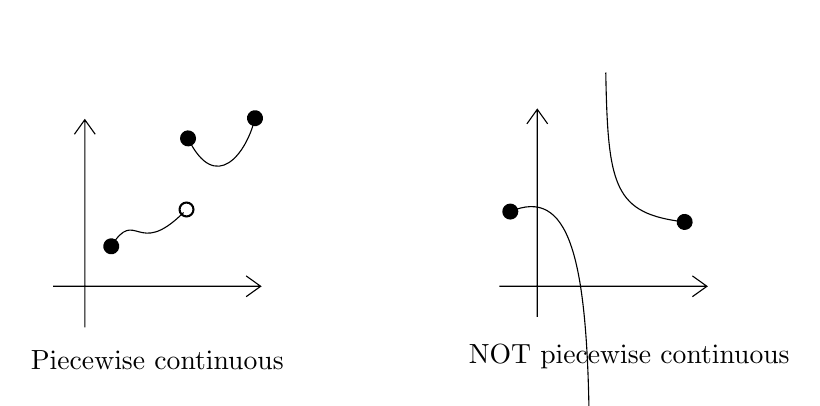
\begin{tikzpicture}[x=0.75pt,y=0.75pt,yscale=-1,xscale=1]
    %uncomment if require: \path (0,300); %set diagram left start at 0, and has height of 300
    
    %Shape: Axis 2D [id:dp7003951674563056] 
    \draw  (50,158.26) -- (150,158.26)(65.26,78) -- (65.26,178) (143,153.26) -- (150,158.26) -- (143,163.26) (60.26,85) -- (65.26,78) -- (70.26,85)  ;
    %Curve Lines [id:da5314714499980906] 
    \draw    (78,139) .. controls (90.01,119.66) and (90.25,145.2) .. (112.84,122.7) ;
    \draw [shift={(114.26,121.26)}, rotate = 313.83] [color=black  ][line width=0.75]      (0, 0) circle [x radius= 3.35, y radius= 3.35]   ;
    \draw [shift={(78,139)}, rotate = 301.84] [color=black  ][fill=black  ][line width=0.75]      (0, 0) circle [x radius= 3.35, y radius= 3.35]   ;
    %Curve Lines [id:da27910409809362413] 
    \draw    (115,87) .. controls (128.26,114.26) and (143.26,94.26) .. (147.26,77.26) ;
    \draw [shift={(147.26,77.26)}, rotate = 283.24] [color=black  ][fill=black  ][line width=0.75]      (0, 0) circle [x radius= 3.35, y radius= 3.35]   ;
    \draw [shift={(115,87)}, rotate = 64.07] [color=black  ][fill=black  ][line width=0.75]      (0, 0) circle [x radius= 3.35, y radius= 3.35]   ;
    %Shape: Axis 2D [id:dp8923800564332263] 
    \draw  (265,158.26) -- (365,158.26)(283.26,73) -- (283.26,173) (358,153.26) -- (365,158.26) -- (358,163.26) (278.26,80) -- (283.26,73) -- (288.26,80)  ;
    %Curve Lines [id:da7330323189044972] 
    \draw    (270.26,122.26) .. controls (298.26,110.26) and (307.26,143.26) .. (308.26,223.26) ;
    \draw [shift={(270.26,122.26)}, rotate = 336.8] [color=black  ][fill=black  ][line width=0.75]      (0, 0) circle [x radius= 3.35, y radius= 3.35]   ;
    %Curve Lines [id:da7451055597374061] 
    \draw    (354.26,127.26) .. controls (320.26,123.26) and (317.26,110.26) .. (316.26,55.26) ;
    \draw [shift={(354.26,127.26)}, rotate = 186.71] [color=black  ][fill=black  ][line width=0.75]      (0, 0) circle [x radius= 3.35, y radius= 3.35]   ;
    
    % Text Node
    \draw (38,188) node [anchor=north west][inner sep=0.75pt]   [align=left] {Piecewise continuous};
    % Text Node
    \draw (249,185) node [anchor=north west][inner sep=0.75pt]   [align=left] {NOT piecewise continuous};
    
    
    \end{tikzpicture}\]

If $\gamma$ is piecewise continuous, then $\int_{a}^{b}\re \gamma(t)\d t$ and $\int_{a}^{b}\im \gamma(t)\d t$ exist. Then we define \textbf{complex integration}:
\[\int_{a}^{b}\gamma(t)\d t = \int_{a}^{b}\re \gamma(t)\d t +i\cdot \int_{a}^{b}\im \gamma(t)\d t\]

That is, \begin{align*}
    \re \left(\int_{a}^{b}\gamma(t)\d t\right)&=\int_{a}^{b}\re \gamma(t)\d t\\
    \im \left(\int_{a}^{b}\gamma(t)\d t\right)&=\int_{a}^{b}\im \gamma(t)\d t\\
\end{align*}

In addition, if $\gamma_1,\gamma_2$ are both $[a,b]\to \C$ and piecewise cont., and $c_1,c_2\in\C$, then \[\int_{a}^{b}\left( c_1\gamma_1(t)+c_2\gamma_2(t) \right)\d t=c_1\int_{a}^{b}\gamma_1(t)\d t+c_2\int_{a}^{b}\gamma_2(t)\d t\]

\addlink{Triangle inequality}
\begin{proposition}[Triangle inequality]
    If $\gamma:[a,b]\to \C$ is {piecewise} continuous, then \[\left|\int_{a}^{b}\gamma(t)\d t \right|\leq \int_{a}^{b}|\gamma(t)|\d t \]
\end{proposition}
\begin{proof}
    WLOG assume $ \int_{a}^{b}\gamma(t)\d t \neq 0$. Define $\lambda = \frac{\left|\int_{a}^{b}\gamma(t)\d t\right|}{\int_{a}^{b}\gamma(t)\d t}$ and note $|\lambda|=1$.

    Thus, \begin{align*}
        \left|\int_{a}^{b}\gamma(t)\d t\right| &= \lambda\int_{a}^{b}\gamma(t)\d t\\
        &= \int_{a}^{b}\lambda\gamma(t)\d t &&\text{because LHS is }\in \R\\
        &= \re \int_{a}^{b}\lambda\gamma(t)\d t\\
        &\leq \int_{a}^{b}|\lambda\gamma(t)|\d t &&\because \re z\leq |z|\\
        &= \int_{a}^{b}|\gamma(t)|\d t&& \because |\lambda|=1
    \end{align*}
\end{proof}

\subsubsection{Complex differentiability}
\defn $\gamma:[a,b]\to \C$ is \textbf{differentiable} at $t\in [a,b]$ if $\re \gamma$ and $\im \gamma$ are differentiable (in the sense of real variables). We define \[\gamma'(t)=(\re \gamma)'(t)+i\cdot (\im \gamma)'(t)\]

\defn $\gamma:[a,b]\to \C$ is \textbf{piecewise} $C^1$\sidenote{$C^1$ is one-time differentiable} if: \begin{enumerate}[label=(\alph*)]
    \item $\gamma$ is continuous on $[a,b]$.
    \item $\gamma$ is differentiable at all but finitely many points of $[a,b]$.
    \item $\gamma'$ is continuous at each point where it exists.
    \item $\gamma'$ has finite one-sided limits at every point of discontinuity.
\end{enumerate}

\subsubsection{Fundamental theorem of calculus, complex edition}
If $\gamma:[a,b]\to\C$ is piecewise $C^1$, then:
\[\int_{a}^{b}\gamma'(t)\d t=\gamma(b)-\gamma(a)\]

\defn If $\gamma$ is $C^1$, then the arclength
\sidenote{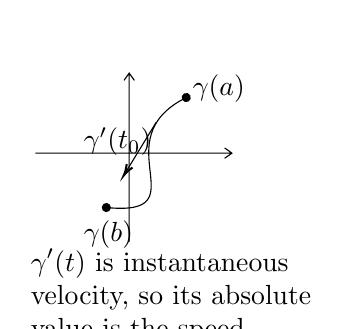
\begin{tikzpicture}[x=0.75pt,y=0.75pt,yscale=-0.5,xscale=0.5]
    %uncomment if require: \path (0,286); %set diagram left start at 0, and has height of 286
    
    %Shape: Axis 2D [id:dp5992461788507699] 
    \draw  (50,141.08) -- (239.26,141.08)(140.26,64) -- (140.26,226.51) (232.26,136.08) -- (239.26,141.08) -- (232.26,146.08) (135.26,71) -- (140.26,64) -- (145.26,71)  ;
    %Curve Lines [id:da8169369769076535] 
    \draw    (118.26,193.51) .. controls (210.26,202.51) and (113.26,128.51) .. (195.26,87.51) ;
    \draw [shift={(195.26,87.51)}, rotate = 333.43] [color=black  ][fill=black  ][line width=0.75]      (0, 0) circle [x radius= 3.35, y radius= 3.35]   ;
    \draw [shift={(118.26,193.51)}, rotate = 5.59] [color=black  ][fill=black  ][line width=0.75]      (0, 0) circle [x radius= 3.35, y radius= 3.35]   ;
    %Straight Lines [id:da7279313778056917] 
    \draw    (166.26,111.51) -- (136.05,160.92) ;
    \draw [shift={(135,162.63)}, rotate = 301.44] [color=black  ][line width=0.75]    (10.93,-3.29) .. controls (6.95,-1.4) and (3.31,-0.3) .. (0,0) .. controls (3.31,0.3) and (6.95,1.4) .. (10.93,3.29)   ;
    
    % Text Node
    \draw (199,63.4) node [anchor=north west][inner sep=0.75pt]    {$\gamma ( a)$};
    % Text Node
    \draw (94,203.4) node [anchor=north west][inner sep=0.75pt]    {$\gamma ( b)$};
    % Text Node
    \draw (94,114.4) node [anchor=north west][inner sep=0.75pt]    {$\gamma '( t_{0})$};
    % Text Node
    \draw (43,231) node [anchor=north west][inner sep=0.75pt]   [align=left] {$\displaystyle \gamma '( t)$ is instantaneous\\ velocity, so its absolute\\ value is the speed};
    
    
    \end{tikzpicture}
    } 
    of $\gamma$ is: \[L(\gamma)=\int_{a}^{b}|\gamma'(t)|\d t\]

\defn If $\gamma:[a,b]\to \reg$ is piecewise $C^1$ and $f:\reg \to\C$ is continuous, then \[\int_{\gamma}f(z)\d z=\int_{a}^{b}f(\gamma(t))\gamma'(t)\d t\]
where $z=\gamma(t)$ and $\d z=\gamma'(t)\d t$

We have \textbf{linearity} w.r.t. $f$: \[\int_{\gamma}\left( c_1f_1(z)+c_2f_2(z) \right)\d z=c_1\int_{\gamma}f_1(z)\d z+c_2\int_{\gamma}f_2(z)\d z\]

\rmk Arclength is independent from parameterization.
\begin{proof}
    Let $\gamma:[a,b]\to \reg$ be piecewise $C^1$. Let $\alpha:[c,d] \to [a,b]$ is an increasing, piecewise $C^1$ surjection such that $\alpha(c)=a, \alpha(d)=b$. Then $\phi=\gamma\circ \alpha:[c,d]\to \reg$ is also piecewise $C^1$. Hence, by substituting $s=\alpha(t), \d s=\alpha'(t)\d t$:
    \begin{align*}
        \int_{\phi}f(z)\d z&=\int_{c}^{d}f(\phi(t))\phi'(t)\d t\\
        &= \int_{c}^{d}f(\gamma(\alpha(t)))\gamma'(\alpha(t))\alpha'(t)\d t\\
        &= \int_{a}^{b}f(\gamma(s))\gamma'(s)\d s\\
        &= \int_{\gamma}f(z)\d z
    \end{align*}
\end{proof}

\subsubsection{An important estimate}
Let $f$ be continuous. Since \(\int_{\gamma}f(z)\d z=\int_{a}^{b}f(\gamma(t))\gamma'(t)\d t\), we observe: \begin{align*}
    \left|\int_{\gamma}f(z)\d z\right|&=\left|\int_{a}^{b}f(\gamma(t))\gamma'(t)\d t\right|\\
    &\leq \int_{a}^{b}|f(\gamma(t))|\,|\gamma'(t)|\d t\\
    &\leq \max_{t\in [a,b]}|f(\gamma(t))| \int_{a}^{b}|\gamma'(t)|\d t\\
    &= \rt{\max_{z\in \gamma}|f(z)|\cdot L(\gamma)}
\end{align*}


\defn If $\gamma:[a,b]\to\C$, the reverse of $\gamma$ is $(-\gamma):[-b,-a]\to\C$ defined by $(-\gamma)(t)=\gamma(-t)$. \sidenote{going around the track backwards} Hence, \[\int_{-\gamma}f(z)\d z= -\int_{\gamma}f(z)\d z\]

\rmk We can also break up the curve and integral the two parts separately: \sidenote{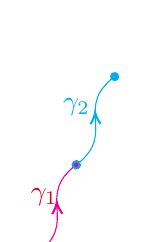
\begin{tikzpicture}[x=0.75pt,y=0.75pt,yscale=-0.5,xscale=0.5]
    %uncomment if require: \path (0,300); %set diagram left start at 0, and has height of 300
    
    %Curve Lines [id:da6510647213107017] 
    \draw [color=magenta  ,draw opacity=1 ]   (144.26,215.76) .. controls (184.26,185.76) and (141.26,160.76) .. (181.26,130.76) ;
    \draw [shift={(181.26,130.76)}, rotate = 323.13] [color=magenta  ,draw opacity=1 ][fill=magenta  ,fill opacity=1 ][line width=0.75]      (0, 0) circle [x radius= 3.35, y radius= 3.35]   ;
    \draw [shift={(162.49,167.07)}, rotate = 87.57] [color=magenta  ,draw opacity=1 ][line width=0.75]    (10.93,-4.9) .. controls (6.95,-2.3) and (3.31,-0.67) .. (0,0) .. controls (3.31,0.67) and (6.95,2.3) .. (10.93,4.9)   ;
    \draw [shift={(144.26,215.76)}, rotate = 323.13] [color=magenta  ,draw opacity=1 ][fill=magenta  ,fill opacity=1 ][line width=0.75]      (0, 0) circle [x radius= 3.35, y radius= 3.35]   ;
    %Curve Lines [id:da6697996530017996] 
    \draw [color=cyan  ,draw opacity=1 ]   (183.56,128.97) .. controls (219.57,99.76) and (179.06,75.16) .. (218.26,45.76) ;
    \draw [shift={(218.26,45.76)}, rotate = 323.13] [color=cyan  ,draw opacity=1 ][fill=cyan  ,fill opacity=1 ][line width=0.75]      (0, 0) circle [x radius= 3.35, y radius= 3.35]   ;
    \draw [shift={(199.47,80.56)}, rotate = 88.14] [color=cyan  ,draw opacity=1 ][line width=0.75]    (10.93,-4.9) .. controls (6.95,-2.3) and (3.31,-0.67) .. (0,0) .. controls (3.31,0.67) and (6.95,2.3) .. (10.93,4.9)   ;
    \draw [shift={(181.26,130.76)}, rotate = 323.13] [color=cyan  ,draw opacity=1 ][line width=0.75]      (0, 0) circle [x radius= 3.35, y radius= 3.35]   ;
    
    % Text Node
    \draw (135,151.4) node [anchor=north west][inner sep=0.75pt]    {$\textcolor[rgb]{0.82,0.01,0.11}{\gamma _{1}}$};
    % Text Node
    \draw (166,64.4) node [anchor=north west][inner sep=0.75pt]    {$\textcolor{cyan}{\gamma _{2}}$};
    
    
    \end{tikzpicture}
    }
\[\int_{\gamma}f(z)\d z = \int_{\gamma_1}f(z)\d z + \int_{\gamma_2}f(z)\d z\]

\subsubsection{Fundamental theorem of calculus for contour integrals}
If $\gamma:[a,b]\to\C$ is piecewise $C^1$, and $f:\reg\to \C$ is analytic \sidenote{Assuming $f'$ continuous, which we would prove later},
then \[\int_{\gamma}f'(z)\d z=f(\gamma(b))-f(\gamma(a))\]

If $\gamma(a)=\gamma(b)$, then $\int_{\gamma}f'(z)\d z=0$.

\begin{proof}
    \begin{align*}
        \int_{\gamma}f'(z)\d z&= \int_{a}^{b}f'(\gamma(t))\gamma'(t)\d t\\
        &= \int_{a}^{b}(f\circ \gamma)'(t)\d t &&\text{chain rule}\\
        &= f(\gamma(b))-f(\gamma(a))
    \end{align*}
\end{proof}

\eg Let $\gamma$ be a circle of radius $R$ centered at $z_0$: $\gamma(t)=z_0+Re^{it}\, ,t\in [0,2\pi]$. We would like to find \(\int_{\gamma}(z-z_0)^n\d z\).

If $n\neq -1$, then $\left(\frac{(z-z_0)^{n+1}}{n+1}\right)' = (z-z_0)^n$. Thus, \[\int_{\gamma}(z-z_0)^n\d z = \int_{\gamma}\left(\frac{(z-z_0)^{n+1}}{n+1}\right)'\d z =0\] by FTC. 

If $n=-1$, \[\int_{\gamma}(z-z_0)^n\d z= \int_{\gamma}\frac{1}{z-z_0}\d z = \int_{0}^{2\pi}i\d t=2\pi i\]

\subsection{Cauchy's theorem}
\subsubsection{Take 1}
\begin{theorem}[Cauchy's]\label[theorem]{cauchys-take1}
    Let $\reg$ be a region in $\C$ containing a \textit{simple}\sidenote{does not self-intersect} piecewise $C^1$ \textit{closed} curve $\gamma$ and its interior\sidenote{holes not allowed in the interior}.

    If $f:\reg \to \C$ is analytic, then $\int_{\gamma}f(z)\d z=0$.
    \[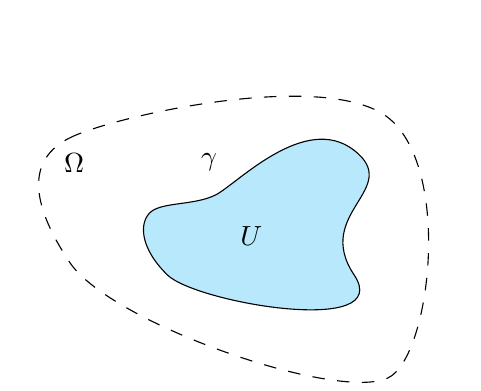
\begin{tikzpicture}[x=0.75pt,y=0.75pt,yscale=-1,xscale=1]
        %uncomment if require: \path (0,300); %set diagram left start at 0, and has height of 300
        
        %Shape: Polygon Curved [id:ds9387894112968782] 
        \draw  [fill=cyan  ,fill opacity=0.28 ] (163.26,91.51) .. controls (173.26,86.51) and (206.26,51.51) .. (230,70) .. controls (253.74,88.49) and (210,100) .. (230,130) .. controls (250,160) and (153.74,143.49) .. (140,130) .. controls (126.26,116.51) and (126.44,104.14) .. (132.26,99.51) .. controls (138.07,94.89) and (153.26,96.51) .. (163.26,91.51) -- cycle ;
        %Shape: Polygon Curved [id:ds6099513547861319] 
        \draw  [dash pattern={on 4.5pt off 4.5pt}] (93,64) .. controls (113,54) and (207.26,32.51) .. (242.26,51.51) .. controls (277.26,70.51) and (268.26,163.51) .. (248.26,178.51) .. controls (228.26,193.51) and (113,154) .. (93,124) .. controls (73,94) and (73,74) .. (93,64) -- cycle ;
        
        % Text Node
        \draw (89,70.4) node [anchor=north west][inner sep=0.75pt]    {${\Omega}$};
        % Text Node
        \draw (174,105.4) node [anchor=north west][inner sep=0.75pt]    {$U$};
        % Text Node
        \draw (155,70.4) node [anchor=north west][inner sep=0.75pt]    {$\gamma $};
        
        
        \end{tikzpicture}
        \]
\end{theorem}
\begin{proof}[``Proof'']
    Let $U$ be the union of $\gamma$ and its interior. Let $f=u+iv$ as usual, write $\d z = \d x + i\d y$:\begin{align*}
        \int_{\gamma}f(z)\d z &= \int_\gamma (u+iv)(\d x + i\d y)\\
        &= \int_\gamma u\d x-v\d y + i\int_{\gamma}v\d x +u\d y\\
        &= \int\int_{U}(-v_x-u_y)\d x\d y+i\int\int_{U}(u_x-v_y)\d x\d y &&\text{by Green's thm}\\
        &= 0 &&\text{by Cauchy-Riemann}
    \end{align*}
\end{proof}
However, this `proof' heavily relies on the fact that $u,v$ are $C^1$ and that the partial derivatives are continuous. This assumes $f'$ is continuous, but we aren't sure about that yet!\sidenote{See \hyperlink{goursats-lemma}{Goursat's Lemma}}

\subsubsection{Take 2: deformation version}
\begin{theorem}[Cauchy's]\label[theorem]{cauchys-take2-deform}
    Let $\gamma_1,\gamma_2$ be piecewise $C^1$ curves in a region $\Omega$ with the same start and end points. If $\gamma_1$ can be continuously deformed to $\gamma_2$ without ever passing outside of $\Omega$, then \[\int_{\gamma_1}f(z)\d z=\int_{\gamma_2}f(z)\d z\]
\end{theorem}
By the \textit{previous} statement of Cauchy's theorem (in \cref{cauchys-take1}), we observe that $\int_{\gamma_1-\gamma_2}f(z)\d z=0$, so this one falls out.

\noneg The $\gamma_1,\gamma_2$ in the picture below cannot be continuously deformed into each other!
\[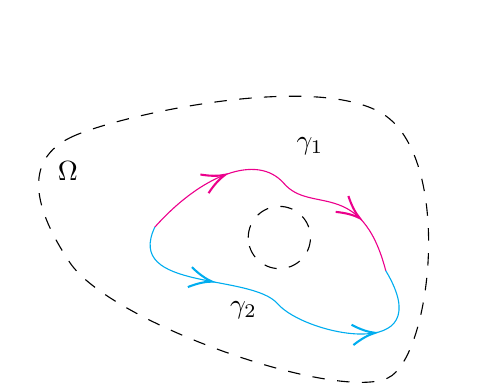
\begin{tikzpicture}[x=0.75pt,y=0.75pt,yscale=-1,xscale=1]
    %uncomment if require: \path (0,300); %set diagram left start at 0, and has height of 300
    
    %Shape: Polygon Curved [id:ds6460613846150254] 
    \draw  [dash pattern={on 4.5pt off 4.5pt}] (116,80) .. controls (136,70) and (230.26,48.51) .. (265.26,67.51) .. controls (300.26,86.51) and (291.26,179.51) .. (271.26,194.51) .. controls (251.26,209.51) and (136,170) .. (116,140) .. controls (96,110) and (96,90) .. (116,80) -- cycle ;
    %Curve Lines [id:da29780021147999514] 
    \draw [color=magenta  ,draw opacity=1 ]   (157,123) .. controls (179.26,98.01) and (206.26,87.01) .. (219.26,102.01) .. controls (232.26,117.01) and (256.51,99.03) .. (268.26,144.01) ;
    \draw [shift={(190.93,97.76)}, rotate = 156.33] [color=magenta  ,draw opacity=1 ][line width=0.75]    (10.93,-4.9) .. controls (6.95,-2.3) and (3.31,-0.67) .. (0,0) .. controls (3.31,0.67) and (6.95,2.3) .. (10.93,4.9)   ;
    \draw [shift={(255.72,118.67)}, rotate = 218.7] [color=magenta  ,draw opacity=1 ][line width=0.75]    (10.93,-4.9) .. controls (6.95,-2.3) and (3.31,-0.67) .. (0,0) .. controls (3.31,0.67) and (6.95,2.3) .. (10.93,4.9)   ;
    %Curve Lines [id:da7249434898522338] 
    \draw [color=cyan  ,draw opacity=1 ]   (157,123) .. controls (142.26,154.01) and (203.26,145.01) .. (216.26,160.01) .. controls (229.26,175.01) and (295.26,189.01) .. (268.26,144.01) ;
    \draw [shift={(184.59,149.25)}, rotate = 191.44] [color=cyan  ,draw opacity=1 ][line width=0.75]    (10.93,-4.9) .. controls (6.95,-2.3) and (3.31,-0.67) .. (0,0) .. controls (3.31,0.67) and (6.95,2.3) .. (10.93,4.9)   ;
    \draw [shift={(263.11,173.95)}, rotate = 174.82] [color=cyan  ,draw opacity=1 ][line width=0.75]    (10.93,-4.9) .. controls (6.95,-2.3) and (3.31,-0.67) .. (0,0) .. controls (3.31,0.67) and (6.95,2.3) .. (10.93,4.9)   ;
    %Shape: Circle [id:dp10939024496763072] 
    \draw  [dash pattern={on 4.5pt off 4.5pt}] (202,128.01) .. controls (202,119.73) and (208.71,113.01) .. (216.99,113.01) .. controls (225.27,113.01) and (231.99,119.73) .. (231.99,128.01) .. controls (231.99,136.29) and (225.27,143) .. (216.99,143) .. controls (208.71,143) and (202,136.29) .. (202,128.01) -- cycle ;
    
    % Text Node
    \draw (109,90.4) node [anchor=north west][inner sep=0.75pt]    {$\Omega $};
    % Text Node
    \draw (224,78.4) node [anchor=north west][inner sep=0.75pt]    {$\gamma _{1}$};
    % Text Node
    \draw (192,157.4) node [anchor=north west][inner sep=0.75pt]    {$\gamma _{2}$};
    
    
    \end{tikzpicture}
    \]

\subsection{Fresnel integrals}
Consider:
\[\int_{0}^{\infty}\sin (t^2)\d t \qquad \text{and} \qquad \int_{0}^{\infty}\cos (t^2)\d t\]
aka.
\[\lim_{R\to \infty}\int_{0}^{R}\sin (t^2)\d t \qquad \text{and} \qquad \lim_{R\to \infty}\int_{0}^{R}\cos (t^2)\d t\]
It's not obvious that these integrals converge!

Solution: PIZZA!
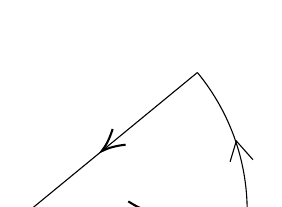
\begin{tikzpicture}[x=0.75pt,y=0.75pt,yscale=-1,xscale=1]
    %uncomment if require: \path (0,300); %set diagram left start at 0, and has height of 300
    
    %Straight Lines [id:da23065699869402656] 
    \draw    (100,126) -- (206.26,126) ;
    \draw [shift={(159.13,126)}, rotate = 180] [color=black  ][line width=0.75]    (10.93,-4.9) .. controls (6.95,-2.3) and (3.31,-0.67) .. (0,0) .. controls (3.31,0.67) and (6.95,2.3) .. (10.93,4.9)   ;
    %Shape: Arc [id:dp010225998094383515] 
    \draw  [draw opacity=0] (205.5,126.02) .. controls (205.5,126.01) and (205.5,126.01) .. (205.5,126) .. controls (205.5,100.56) and (196.5,77.23) .. (181.5,59.01) -- (100,126) -- cycle ; \draw   (205.5,126.02) .. controls (205.5,126.01) and (205.5,126.01) .. (205.5,126) .. controls (205.5,100.56) and (196.5,77.23) .. (181.5,59.01) ;  
    %Straight Lines [id:da5834097312816091] 
    \draw    (100,126) -- (181.5,59.01) ;
    \draw [shift={(135.34,96.95)}, rotate = 320.58] [color=black  ][line width=0.75]    (10.93,-4.9) .. controls (6.95,-2.3) and (3.31,-0.67) .. (0,0) .. controls (3.31,0.67) and (6.95,2.3) .. (10.93,4.9)   ;
    %Straight Lines [id:da6100230617755076] 
    \draw    (197.26,102.01) -- (200.26,92.01) -- (208.26,101.01) ;
    
    
    
    
    \end{tikzpicture}
Let $\gamma$ be the `sum' of all 3 curves as shown. Let $R\to \infty$. Then, by Cauchy's theorem, \(\int_\gamma e^{iz^2}\d z =0\).    

\ontangent{

\rmk We don't know how to write out the antiderivative of $f(z)=e^{iz^2}$ but we can use series!
\begin{align*}
    f(z) &= e^{iz^2}\\
    &= \sum_{n=0}^{\infty}\frac{(iz^2)^n}{n!}\\
    &= \sum_{n=0}^{\infty}\frac{i^nz^{2n}}{n!}
\end{align*}
And so \[F(z)=\sum_{n=0}^{\infty}\frac{i^nz^{2n+1}}{(2n+1)n!}\]

}

Now we return to the integral. Strategy: \[0= \int_\gamma e^{iz^2}\d  = \underset{I_1(R)}{\underbrace{\int_{\gamma_1} e^{iz^2}\d z}} + \underset{I_2(R)}{\underbrace{\int_{\gamma_2} e^{iz^2}\d z}} + \underset{I_3(R)}{\underbrace{\int_{\gamma_3} e^{iz^2}\d z}}\]

\[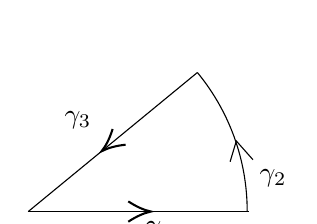
\begin{tikzpicture}[x=0.75pt,y=0.75pt,yscale=-1,xscale=1]
    %uncomment if require: \path (0,300); %set diagram left start at 0, and has height of 300
    
    %Straight Lines [id:da23065699869402656] 
    \draw    (100,126) -- (206.26,126) ;
    \draw [shift={(159.13,126)}, rotate = 180] [color=black  ][line width=0.75]    (10.93,-4.9) .. controls (6.95,-2.3) and (3.31,-0.67) .. (0,0) .. controls (3.31,0.67) and (6.95,2.3) .. (10.93,4.9)   ;
    %Shape: Arc [id:dp010225998094383515] 
    \draw  [draw opacity=0] (205.5,126.02) .. controls (205.5,126.01) and (205.5,126.01) .. (205.5,126) .. controls (205.5,100.56) and (196.5,77.23) .. (181.5,59.01) -- (100,126) -- cycle ; \draw   (205.5,126.02) .. controls (205.5,126.01) and (205.5,126.01) .. (205.5,126) .. controls (205.5,100.56) and (196.5,77.23) .. (181.5,59.01) ;  
    %Straight Lines [id:da5834097312816091] 
    \draw    (100,126) -- (181.5,59.01) ;
    \draw [shift={(135.34,96.95)}, rotate = 320.58] [color=black  ][line width=0.75]    (10.93,-4.9) .. controls (6.95,-2.3) and (3.31,-0.67) .. (0,0) .. controls (3.31,0.67) and (6.95,2.3) .. (10.93,4.9)   ;
    %Straight Lines [id:da6100230617755076] 
    \draw    (197.26,102.01) -- (200.26,92.01) -- (208.26,101.01) ;
    
    % Text Node
    \draw (155.13,129.4) node [anchor=north west][inner sep=0.75pt]    {$\gamma _{1}$};
    % Text Node
    \draw (210.26,104.41) node [anchor=north west][inner sep=0.75pt]    {$\gamma _{2}$};
    % Text Node
    \draw (116.26,76.41) node [anchor=north west][inner sep=0.75pt]    {$\gamma _{3}$};
    
    
    \end{tikzpicture}
    \]

Evaluate $I_1(R)$: We observe that $z$ is real for this one. Parameterize $z=t$ where $t$ is a real variable.
\begin{align*}
    I_1(R) &= \int_{\gamma_1} e^{it^2}\d t\\
    &= \int_{0}^{R}\cos (t^2)\d t + i\cdot \int_{0}^{R}\sin (t^2)\d t\\
\end{align*}
Hence, $\lim_{R\to \infty}I_1(R)= \int_{0}^{\infty}\cos (t^2)\d t + i\cdot \int_{0}^{\infty}\sin (t^2)\d t$.

Evaluate $I_2(R)$:

Parameterize $\gamma_2$ as $z=Re^{i\theta}$ where $\theta\in[0,\frac{\pi}{4}]$. Hence, $\d z = iRe^{i\theta}\d \theta$. Then:
\begin{align*}
    |I_2(R)| &= \left|\int_{\gamma_2} e^{i\theta^2}\d \theta\right|\\
    &= \left|\int_{0}^{\frac{\pi}{4}}e^{i(R e^{i\theta})^2}iRe^{i\theta}\d \theta\right|\\
    &= \left|R\int_{0}^{\frac{\pi}{4}}e^{iR^2e^{i2\theta}}e^{i\theta}\d \theta\right|\\
    &\leq R\int_{0}^{\frac{\pi}{4}}\left|e^{iR^2e^{i2\theta}}\right|\d \theta &&\text{by tri. ineq.}\\
    &\leq R\int_{0}^{\frac{\pi}{4}}e^{-R^2\sin2\theta}\d \theta&&\text{since when }x,y\in \R,\; \left|e^{x+iy}\right|=e^{x}\\
    &\leq  R\int_{0}^{\frac{\pi}{4}} e^{-R^2\frac{4\theta}{\pi}}\d \theta &&\text{since when }x\in [0,\frac{\pi}{2}],\; \frac{2}{\pi}x\leq \sin x\\
    &= \frac{-R\pi}{R^2 4}e^{-R\frac{4\theta}{\pi}}\bigg |_{\theta=0}^{\theta=\frac{\pi}{4}}\\
    &\to 0 \text{ as }R\to \infty
\end{align*}
Thus, $\lim_{R\to \infty}I_2(R)=0$. :)

Evaluate $I_3(R)$:
\begin{align*}
    I_3(R) &=\int_{\gamma_3} e^{iz^2}\d z\\
    &= \int_{R}^{0}e^{i(e^{i\frac{\pi}{4}}t)^2}e^{i\frac{\pi}{4}}\d t\\
    &= -e^{i\frac{\pi}{4}} \int_{0}^{R}e^{-t^2}\d t\\
    \lim_{R\to \infty} I_3(R) &= -(\frac{\sqrt{2}}{2}+i\frac{\sqrt{2}}{2})\int_{0}^{\infty}e^{-t^2}\d t &&\text{by Gaussian integral, }\int_{0}^{\infty}e^{-t^2}\d t = \frac{\sqrt{\pi}}{2}\\
    &= -\sqrt{\frac{\pi}{8}}-i\sqrt{\frac{\pi}{8}}
\end{align*}

Therefore, we see $I_1(R)+I_2(R)+I_3(R)=0$ where $\lim_{R\to \infty}I_1(R)= \int_{0}^{\infty}\cos (t^2)\d t + i\cdot \int_{0}^{\infty}\sin (t^2)\d t$, $I_2(R)\to 0$ and $I_3(R)= -\sqrt{\frac{\pi}{8}}-i\sqrt{\frac{\pi}{8}}$. Hence, we would be able to conclude that \[\int_{0}^{\infty}\sin (t^2)\d t = \sqrt{\frac{\pi}{8}} \qquad \text{and} \qquad \int_{0}^{\infty}\cos (t^2)\d t = \sqrt{\frac{\pi}{8}}\]

\subsection{Goursat's lemma}
This lemma patches the hole that we have to assume $f'$ continuous in Cauchy's theorem!
\begin{lemma}[Goursat's]
    \hypertarget{goursats-lemma}{If} $f:\Omega\to \C$ is analytic and $\Delta$ is a triangle in $\reg$ whose interior lies inside $\Omega$, then $\int_{\Delta}f(z)\d z=0$.\sidenote{Does not assume $f'$ continuous!}
\end{lemma}
\begin{proof}
    WLOG orient $\Delta_0=\Delta$ counterclockwise. Bisect sides of $\Delta_0$ and construct smaller triangles $\Delta_{0j}$ where $j=1,2,3,4$. Then, \[I=\int_{\Delta_0}f(z)\d z=\sum_{j=1}^{4}\int_{\Delta_{0j}}f(z)\d z\]
    \[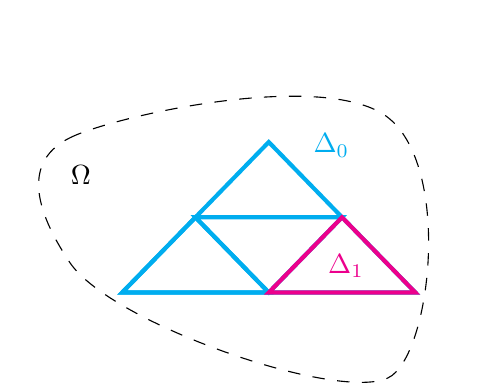
\begin{tikzpicture}[x=0.75pt,y=0.75pt,yscale=-1,xscale=1]
        %uncomment if require: \path (0,300); %set diagram left start at 0, and has height of 300
        
        %Shape: Triangle [id:dp00827622632180569] 
        \draw  [color=cyan  ,draw opacity=1 ][line width=1.5]  (170.63,87.51) -- (241.26,160) -- (100,160) -- cycle ;
        %Shape: Polygon Curved [id:ds3012264222748664] 
        \draw  [dash pattern={on 4.5pt off 4.5pt}] (74.74,85.49) .. controls (94.74,75.49) and (189,54) .. (224,73) .. controls (259,92) and (250,185) .. (230,200) .. controls (210,215) and (94.74,175.49) .. (74.74,145.49) .. controls (54.74,115.49) and (54.74,95.49) .. (74.74,85.49) -- cycle ;
        %Shape: Triangle [id:dp8224876385734627] 
        \draw  [color=cyan  ,draw opacity=1 ][line width=1.5]  (135.31,123.76) -- (170.63,160) -- (100,160) -- cycle ;
        %Shape: Triangle [id:dp8894284388389209] 
        \draw  [color=cyan  ,draw opacity=1 ][line width=1.5]  (170.63,160) -- (135.31,123.76) -- (205.94,123.76) -- cycle ;
        %Shape: Triangle [id:dp25960520730846914] 
        \draw  [color=magenta  ,draw opacity=1 ][line width=1.5]  (205.94,123.76) -- (241.26,160) -- (170.63,160) -- cycle ;
        
        % Text Node
        \draw (74,97.4) node [anchor=north west][inner sep=0.75pt]    {$\Omega $};
        % Text Node
        \draw (198,140.4) node [anchor=north west][inner sep=0.75pt]  [color=magenta  ,opacity=1 ]  {$\Delta _{1}$};
        % Text Node
        \draw (191,82.4) node [anchor=north west][inner sep=0.75pt]  [color=cyan  ,opacity=1 ]  {$\Delta _{0}$};
        
        
        \end{tikzpicture}
        \]
    By triangle inequality, \[|I|\leq \sum_{j=1}^{4}\left|\int_{\Delta_{0j}}f(z)\d z\right|\]
    Thus, there exists $j\in \{1,2,3,4\}$ such that \[\frac{|I|}{4}\leq \left|\int_{\Delta_{0j}}f(z)\d z\right|\]
    For this $j$, define $\Delta_1=\Delta_{0j}$.

    We disect $\Delta_1$ again into smaller triangles $\Delta_{1j}$ where $j=1,2,3,4$. Then, \[I=\int_{\Delta_1}f(z)\d z=\sum_{j=1}^{4}\int_{\Delta_{1j}}f(z)\d z\]
    Again, by triangle inequality, there is a $j\in \{1,2,3,4\}$ such that \[\rt{\frac{|I|}{4^2}}\leq \frac{1}{4}\left|\int_{\Delta_1}f(z)\d z\right|\leq \left|\int_{\Delta_{1j}}f(z)\d z\right|\]
    For this $j$, define $\Delta_2=\Delta_{1j}$.

    \[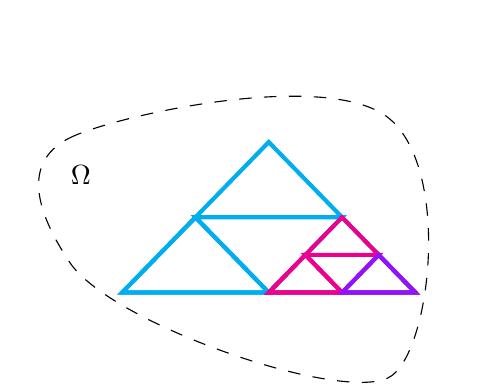
\begin{tikzpicture}[x=0.75pt,y=0.75pt,yscale=-1,xscale=1]
        %uncomment if require: \path (0,300); %set diagram left start at 0, and has height of 300
        
        %Shape: Triangle [id:dp00827622632180569] 
        \draw  [color=cyan  ,draw opacity=1 ][line width=1.5]  (170.63,87.51) -- (241.26,160) -- (100,160) -- cycle ;
        %Shape: Polygon Curved [id:ds3012264222748664] 
        \draw  [dash pattern={on 4.5pt off 4.5pt}] (74.74,85.49) .. controls (94.74,75.49) and (189,54) .. (224,73) .. controls (259,92) and (250,185) .. (230,200) .. controls (210,215) and (94.74,175.49) .. (74.74,145.49) .. controls (54.74,115.49) and (54.74,95.49) .. (74.74,85.49) -- cycle ;
        %Shape: Triangle [id:dp8224876385734627] 
        \draw  [color=cyan  ,draw opacity=1 ][line width=1.5]  (135.31,123.76) -- (170.63,160) -- (100,160) -- cycle ;
        %Shape: Triangle [id:dp8894284388389209] 
        \draw  [color=cyan  ,draw opacity=1 ][line width=1.5]  (170.63,160) -- (135.31,123.76) -- (205.94,123.76) -- cycle ;
        %Shape: Triangle [id:dp25960520730846914] 
        \draw  [color=magenta  ,draw opacity=1 ][line width=1.5]  (205.94,123.76) -- (241.26,160) -- (170.63,160) -- cycle ;
        %Shape: Triangle [id:dp9594922625539553] 
        \draw  [color=magenta  ,draw opacity=1 ][line width=1.5]  (188.28,141.88) -- (205.94,160) -- (170.63,160) -- cycle ;
        %Shape: Triangle [id:dp41273457544096503] 
        \draw  [color=magenta  ,draw opacity=1 ][line width=1.5]  (205.94,160) -- (188.28,141.88) -- (223.6,141.88) -- cycle ;
        %Shape: Triangle [id:dp4722169823972482] 
        \draw  [color={rgb, 255:red, 144; green, 19; blue, 254 }  ,draw opacity=1 ][line width=1.5]  (223.6,141.88) -- (241.26,160) -- (205.94,160) -- cycle ;
        
        % Text Node
        \draw (74,97.4) node [anchor=north west][inner sep=0.75pt]    {$\Omega $};
        
        
        \end{tikzpicture}        
        \]

    \dots continue in this manner to get nested triangles $\Delta_n$ such that \[\rt{\frac{|I|}{4^{n+1}}}\leq \frac{1}{4}\left|\int_{\Delta_n}f(z)\d z\right|\leq \left|\int_{\Delta_{nj}}f(z)\d z\right|\] for all $n\geq 0$.

    Now let $\ell=L(\Delta_0)$ denote perimeter of the original triangle (blue).\\ Then $L(\Delta_n)=\frac{\ell}{2^n}$\sidenote{Perimeter of $\Delta_n$}. 

    Let $K_n$ denote the triangle $\Delta_n$ union with its interior such that $K_n$ is closed (in fact, compact!). Let $\zeta_n\in K_n$ for $n\geq 0$. Then there is $N\in \N$, such that for all $m,n\geq N$ we have $|\zeta_m-\zeta_n|\leq \operatorname{diam}(K_N)\leq \frac{\ell}{2^N}$. Thus, $\zeta_n$ as a sequence is Cauchy.

    Let $z_0=\lim_{n\to\infty}\zeta_n$, note $z_0\in \bigcap_{n=0}^{\infty} K_n$ and $z_0\in \Omega$. Since $f$ is analytic at $z_0$, given $\varepsilon>0$, there exists some $\delta>0$ such that whenever $|z-z_0|<\delta$, we have \[\left|\frac{f(z)-f(z_0)}{z-z_0}-f'(z_0)\right|<\frac{\varepsilon}{\ell^2}\]

    Now consider multiplying $|z-z_0|$ on both sides:
    \begin{align*}
        |f'(z_0)\cdot (z-z_0) - f(z) + f(z_0)| &< \frac{\varepsilon}{\ell^2} |z-z_0|\\
        |f(z_0) + f'(z_0)(z-z_0)-f(z)| &<\frac{\varepsilon}{\ell^2} |z-z_0|
    \end{align*}
    Since $f(z_0) + f'(z_0)(z-z_0)$ is \textbf{linear}, it has an antiderivative on $\C$. Thus, \[\int_{\Delta_n}f(z_0) + f'(z_0)(z-z_0)\d z = 0\]
    by FTC! Now pick $n$ large enough so that $|z-z_0<\delta$ for all $z\in \Delta_n$. Thus, \begin{align*}
        |I|&\leq 4^n \left|\int_{\Delta_n}f(z)\d z\right|\\ 
        &= 4^n\left|\int_{\Delta_n}f(z_0) + f'(z_0)(z-z_0)-f(z)\right|\\
        &\leq 4^n\frac{\varepsilon}{\ell^2}|z-z_0|\frac{\ell}{2^n} &&\text{by tri. ineq. and }\left|\int_\gamma g(z)\d z\right|\leq \sup_{z\in \gamma}|g(z)|\cdot L(\gamma)\\
        &< \frac{4^n\varepsilon}{\ell 2^n}\cdot \frac{\ell}{2^n}\\
        &= \varepsilon
    \end{align*}

   
\end{proof}

\subsubsection{Local antiderivative}
\begin{theorem}\label[theorem]{convex-antiderivative}
    If $\reg$ is convex and $f:\reg \to \C$ is analytic, then $f$ has an antiderivative on $\reg$.
\end{theorem}
\rmk Line segments don't exit the region in convex shapes:\[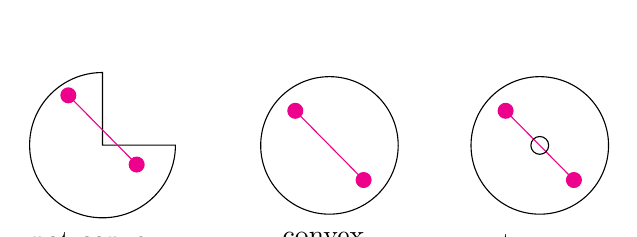
\begin{tikzpicture}[x=0.75pt,y=0.75pt,yscale=-1,xscale=1]
    %uncomment if require: \path (0,300); %set diagram left start at 0, and has height of 300
    
    %Shape: Pie [id:dp6860240797492949] 
    \draw   (136.92,115.67) .. controls (136.92,115.67) and (136.92,115.67) .. (136.92,115.67) .. controls (136.92,135) and (121.19,150.67) .. (101.79,150.67) .. controls (82.39,150.67) and (66.67,135) .. (66.67,115.67) .. controls (66.67,96.34) and (82.39,80.67) .. (101.79,80.67) -- (101.79,115.67) -- cycle ;
    %Straight Lines [id:da6856373582050304] 
    \draw [color=magenta  ,draw opacity=1 ]   (85.33,91.67) -- (118.25,125.01) ;
    \draw [shift={(118.25,125.01)}, rotate = 45.36] [color=magenta  ,draw opacity=1 ][fill=magenta  ,fill opacity=1 ][line width=0.75]      (0, 0) circle [x radius= 3.35, y radius= 3.35]   ;
    \draw [shift={(85.33,91.67)}, rotate = 45.36] [color=magenta  ,draw opacity=1 ][fill=magenta  ,fill opacity=1 ][line width=0.75]      (0, 0) circle [x radius= 3.35, y radius= 3.35]   ;
    %Shape: Circle [id:dp6630767252853171] 
    \draw   (178,115.79) .. controls (178,97.5) and (192.83,82.67) .. (211.13,82.67) .. controls (229.42,82.67) and (244.25,97.5) .. (244.25,115.79) .. controls (244.25,134.09) and (229.42,148.92) .. (211.13,148.92) .. controls (192.83,148.92) and (178,134.09) .. (178,115.79) -- cycle ;
    %Shape: Circle [id:dp7587345978022606] 
    \draw   (279.33,115.79) .. controls (279.33,97.5) and (294.16,82.67) .. (312.46,82.67) .. controls (330.76,82.67) and (345.59,97.5) .. (345.59,115.79) .. controls (345.59,134.09) and (330.76,148.92) .. (312.46,148.92) .. controls (294.16,148.92) and (279.33,134.09) .. (279.33,115.79) -- cycle ;
    %Straight Lines [id:da09760158868609392] 
    \draw [color=magenta  ,draw opacity=1 ]   (194.67,99.12) -- (227.59,132.47) ;
    \draw [shift={(227.59,132.47)}, rotate = 45.36] [color=magenta  ,draw opacity=1 ][fill=magenta  ,fill opacity=1 ][line width=0.75]      (0, 0) circle [x radius= 3.35, y radius= 3.35]   ;
    \draw [shift={(194.67,99.12)}, rotate = 45.36] [color=magenta  ,draw opacity=1 ][fill=magenta  ,fill opacity=1 ][line width=0.75]      (0, 0) circle [x radius= 3.35, y radius= 3.35]   ;
    %Straight Lines [id:da4239725771757499] 
    \draw [color=magenta  ,draw opacity=1 ]   (296,99.12) -- (328.92,132.47) ;
    \draw [shift={(328.92,132.47)}, rotate = 45.36] [color=magenta  ,draw opacity=1 ][fill=magenta  ,fill opacity=1 ][line width=0.75]      (0, 0) circle [x radius= 3.35, y radius= 3.35]   ;
    \draw [shift={(296,99.12)}, rotate = 45.36] [color=magenta  ,draw opacity=1 ][fill=magenta  ,fill opacity=1 ][line width=0.75]      (0, 0) circle [x radius= 3.35, y radius= 3.35]   ;
    %Shape: Circle [id:dp6744384543792539] 
    \draw   (308.17,115.79) .. controls (308.17,113.43) and (310.09,111.5) .. (312.46,111.5) .. controls (314.83,111.5) and (316.75,113.43) .. (316.75,115.79) .. controls (316.75,118.16) and (314.83,120.08) .. (312.46,120.08) .. controls (310.09,120.08) and (308.17,118.16) .. (308.17,115.79) -- cycle ;
    
    % Text Node
    \draw (66,156.67) node [anchor=north west][inner sep=0.75pt]   [align=left] {not convex};
    % Text Node
    \draw (187.33,156.67) node [anchor=north west][inner sep=0.75pt]   [align=left] {convex};
    % Text Node
    \draw (278.67,157.33) node [anchor=north west][inner sep=0.75pt]   [align=left] {not convex};
    
    
    \end{tikzpicture}
    \]
\begin{proof}
    Fix $w\in \reg$ and define: \[F(z)=\int_{[w,z]}f(\zeta)\d \zeta\] for $z\in \reg$.\sidenote{$[w,z]$ is the line segment from $w$ to $z$.}

    This is well-defined if $\reg$ is convex.

    Now we \dashuline{want to show} that $F'$ is $f$. That is equivalent to showing that for all $\varepsilon>0, z_0\in \reg$, there exists $\delta>0$ s.t. whenever $|z-z_0|<\delta$, we have  \[\left|\frac{F(z)-F(z_0)}{z-z_0}-f(z_0)\right|<{\varepsilon}\]
    Let $z_0\in \Omega$ be given and $\varepsilon>0$. Goursat says integrals around the triangle is 0, so we suppose $z\in \reg\backslash\{z_0,w\}$ and get a triangle:
    \[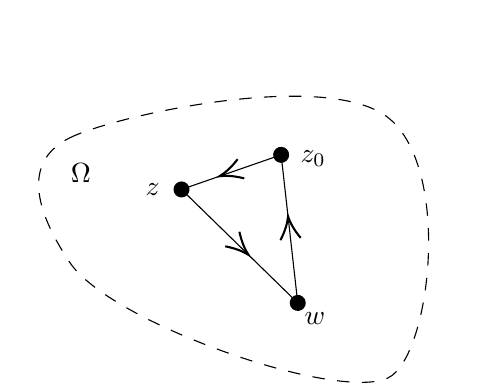
\begin{tikzpicture}[x=0.75pt,y=0.75pt,yscale=-1,xscale=1]
        %uncomment if require: \path (0,300); %set diagram left start at 0, and has height of 300
        
        %Shape: Polygon Curved [id:ds8013551056257879] 
        \draw  [dash pattern={on 4.5pt off 4.5pt}] (94.74,106.15) .. controls (114.74,96.15) and (209,74.67) .. (244,93.67) .. controls (279,112.67) and (270,205.67) .. (250,220.67) .. controls (230,235.67) and (114.74,196.15) .. (94.74,166.15) .. controls (74.74,136.15) and (74.74,116.15) .. (94.74,106.15) -- cycle ;
        %Straight Lines [id:da8523806034462806] 
        \draw    (148.59,131.01) -- (204.59,185.68) ;
        \draw [shift={(180.88,162.53)}, rotate = 224.31] [color=black  ][line width=0.75]    (10.93,-4.9) .. controls (6.95,-2.3) and (3.31,-0.67) .. (0,0) .. controls (3.31,0.67) and (6.95,2.3) .. (10.93,4.9)   ;
        \draw [shift={(148.59,131.01)}, rotate = 44.31] [color=black  ][fill=black  ][line width=0.75]      (0, 0) circle [x radius= 3.35, y radius= 3.35]   ;
        %Straight Lines [id:da16858040739980074] 
        \draw    (204.59,185.68) -- (196.59,114.34) ;
        \draw [shift={(199.92,144.05)}, rotate = 83.6] [color=black  ][line width=0.75]    (10.93,-4.9) .. controls (6.95,-2.3) and (3.31,-0.67) .. (0,0) .. controls (3.31,0.67) and (6.95,2.3) .. (10.93,4.9)   ;
        \draw [shift={(204.59,185.68)}, rotate = 263.6] [color=black  ][fill=black  ][line width=0.75]      (0, 0) circle [x radius= 3.35, y radius= 3.35]   ;
        %Straight Lines [id:da12021387715434817] 
        \draw    (196.59,114.34) -- (148.59,131.01) ;
        \draw [shift={(166.92,124.64)}, rotate = 340.85] [color=black  ][line width=0.75]    (10.93,-4.9) .. controls (6.95,-2.3) and (3.31,-0.67) .. (0,0) .. controls (3.31,0.67) and (6.95,2.3) .. (10.93,4.9)   ;
        \draw [shift={(196.59,114.34)}, rotate = 160.85] [color=black  ][fill=black  ][line width=0.75]      (0, 0) circle [x radius= 3.35, y radius= 3.35]   ;
        
        % Text Node
        \draw (94,117.4) node [anchor=north west][inner sep=0.75pt]    {$\Omega $};
        % Text Node
        \draw (130,127.07) node [anchor=north west][inner sep=0.75pt]    {$z$};
        % Text Node
        \draw (204.67,111.07) node [anchor=north west][inner sep=0.75pt]    {$z_{0}$};
        % Text Node
        \draw (206.59,189.08) node [anchor=north west][inner sep=0.75pt]    {$w$};
        
        
        \end{tikzpicture}
        \]
        and we know that \[\underset{F(z_0)}{\underbrace{\int_{[w,z_0]}f(\zeta)\d \zeta}} + \int_{[z_0,z]}f(\zeta)\d \zeta + \underset{-F(z)}{\underbrace{\int_{[z,w]}f(\zeta)\d \zeta}}=0\]
        So $F(z)-F(z_0)=\int_{[z_0,z]}f(\zeta)\d \zeta$. Thus,
        \begin{align*}
            \frac{F(z)-F(z_0)}{z-z_0}\rt{-f(z_0)} &= \frac{1}{z-z_0}\int_{[z_0,z]}\left(f(\zeta)-f(z_0)\right)\d \zeta
        \end{align*}
        Since $f$ is analytic at $z_0$, it is continuous there. Given $\varepsilon>0$, there exists $\delta>0$ such that whenever $|z-z_0|<\delta$, we have  \(\left|f(z)-f(z_0)\right|<{\varepsilon}\).

        Therefore, whenever $|z-z_0|<\delta$, we have \sidenote{still by \(\left|\int_\gamma g(z)\d z\right|\leq \sup_{z\in \gamma}|g(z)|\cdot L(\gamma)\)}\begin{align*}
            \left|\frac{F(z)-F(z_0)}{z-z_0}-f(z_0)\right| &\leq \frac{\varepsilon}{|z-z_0|}L([z_0,z])\\
            &= \frac{\varepsilon}{|z-z_0|}|z-z_0|\\
            &= \varepsilon
        \end{align*}
\end{proof}

\subsection{Cauchy's theorem, Take 3}
\subsubsection{Cauchy's theorem for convex regions}
\begin{theorem}
    If $\reg$ is convex, $f:\reg\to \C$ analytic and $\gamma$ is a piecewise $C^1$ curve in $\reg$, then $\int_{\gamma}f(z)\d z=0$.\sidenote{Since $\reg$ is convex, the interior of $\gamma$ lies inside $\reg$.}
\end{theorem}
\begin{proof}
    Previous theorem says $f$ has an antiderivative $F$ on $\reg$. Thus, \[\int_{\gamma}f(z)\d z = \int_{\gamma}F'(z)\d z=0\] by FTC!
\end{proof}

\subsection{Cauchy's integral formula}
\subsubsection{Cauchy's integral formula for a circle}
\hypertarget{cauchys-integral-formula}{}
\begin{theorem}\label[theorem]{cif}
    If $f$ is analytic on a region $\Omega$ that contains the circle $\gamma$ and its interior, then \[f(z)=\frac{1}{2\pi i}\int_{\gamma}\frac{f(\zeta)\d \zeta}{\zeta-z}\] for all $z$ inside of $\gamma$.\sidenote{this $\reg$ doesn't need to be convex}
\end{theorem}
\begin{proof}
    Let $r>0$ be small enough so that the closed ball $B_r(z)^-$ is in the interior of $\gamma$. Let $C_r(z)=\{\zeta\in\C :|\zeta-z|=r\}$ traversed clockwise.
    \[\begin{tikzpicture}[x=0.75pt,y=0.75pt,yscale=-0.75,xscale=0.75]
        %uncomment if require: \path (0,300); %set diagram left start at 0, and has height of 300
        
        %Shape: Polygon Curved [id:ds2869580135529062] 
        \draw  [dash pattern={on 4.5pt off 4.5pt}] (85.36,55.55) .. controls (125.83,35.31) and (316.58,-8.17) .. (387.41,30.28) .. controls (458.25,68.73) and (440.03,256.94) .. (399.56,287.29) .. controls (359.08,317.65) and (125.83,237.68) .. (85.36,176.97) .. controls (44.88,116.26) and (44.88,75.78) .. (85.36,55.55) -- cycle ;
        %Shape: Ellipse [id:dp5518722967005327] 
        \draw   (198.69,145.86) .. controls (198.69,93.75) and (240.93,51.5) .. (293.05,51.5) .. controls (345.17,51.5) and (387.41,93.75) .. (387.41,145.86) .. controls (387.41,197.98) and (345.17,240.23) .. (293.05,240.23) .. controls (240.93,240.23) and (198.69,197.98) .. (198.69,145.86) -- cycle ;
        %Shape: Arc [id:dp14115450919361172] 
        \draw  [draw opacity=0] (362.61,130.43) .. controls (362.61,158.37) and (339.96,181.02) .. (312.02,181.02) .. controls (284.07,181.02) and (261.42,158.37) .. (261.42,130.43) .. controls (261.42,102.48) and (284.07,79.83) .. (312.02,79.83) .. controls (339.66,79.83) and (362.13,102.01) .. (362.6,129.54) -- (312.02,130.43) -- cycle ; \draw    (362.61,130.43) .. controls (362.61,158.37) and (339.96,181.02) .. (312.02,181.02) .. controls (284.07,181.02) and (261.42,158.37) .. (261.42,130.43) .. controls (261.42,102.48) and (284.07,79.83) .. (312.02,79.83) .. controls (339.11,79.83) and (361.23,101.13) .. (362.55,127.9) ; \draw [shift={(362.6,129.54)}, rotate = 269.02] [color=black  ][line width=0.75]    (10.93,-3.29) .. controls (6.95,-1.4) and (3.31,-0.3) .. (0,0) .. controls (3.31,0.3) and (6.95,1.4) .. (10.93,3.29)   ; 
        %Straight Lines [id:da08707833068540416] 
        \draw    (312.02,79.83) -- (312.02,130.43) ;
        \draw [shift={(312.02,130.43)}, rotate = 90] [color=black  ][fill=black  ][line width=0.75]      (0, 0) circle [x radius= 3.35, y radius= 3.35]   ;
        
        % Text Node
        \draw (79.38,84.37) node [anchor=north west][inner sep=0.75pt]    {$\Omega $};
        % Text Node
        \draw (196.73,60.09) node [anchor=north west][inner sep=0.75pt]    {$\gamma $};
        % Text Node
        \draw (322.21,145.09) node [anchor=north west][inner sep=0.75pt]    {$z$};
        % Text Node
        \draw (300.95,99.47) node [anchor=north west][inner sep=0.75pt]    {$r$};
        
        
        \end{tikzpicture}
        \]

        Construct $\gamma_1,\gamma_2,\gamma_3,\gamma_4$ as pictured:
        \[\begin{tikzpicture}[x=0.75pt,y=0.75pt,yscale=-1,xscale=1]
            %uncomment if require: \path (0,300); %set diagram left start at 0, and has height of 300
            
            %Shape: Polygon Curved [id:ds2869580135529062] 
            \draw  [dash pattern={on 4.5pt off 4.5pt}] (85.36,55.55) .. controls (125.83,35.31) and (316.58,-8.17) .. (387.41,30.28) .. controls (458.25,68.73) and (440.03,256.94) .. (399.56,287.29) .. controls (359.08,317.65) and (125.83,237.68) .. (85.36,176.97) .. controls (44.88,116.26) and (44.88,75.78) .. (85.36,55.55) -- cycle ;
            %Shape: Arc [id:dp4628794505771803] 
            \draw  [draw opacity=0] (387.41,145.86) .. controls (387.41,145.86) and (387.41,145.86) .. (387.41,145.86) .. controls (387.41,197.98) and (345.17,240.23) .. (293.05,240.23) .. controls (240.93,240.23) and (198.69,197.98) .. (198.69,145.86) .. controls (198.69,93.75) and (240.93,51.5) .. (293.05,51.5) .. controls (344.62,51.5) and (386.52,92.86) .. (387.4,144.22) -- (293.05,145.86) -- cycle ; \draw    (387.41,145.86) .. controls (387.41,197.98) and (345.17,240.23) .. (293.05,240.23) .. controls (240.93,240.23) and (198.69,197.98) .. (198.69,145.86) .. controls (198.69,93.75) and (240.93,51.5) .. (293.05,51.5) .. controls (344.62,51.5) and (386.52,92.86) .. (387.4,144.22) ;  \draw [shift={(387.41,145.86)}, rotate = 90] [color=black  ][line width=0.75]    (10.93,-4.9) .. controls (6.95,-2.3) and (3.31,-0.67) .. (0,0) .. controls (3.31,0.67) and (6.95,2.3) .. (10.93,4.9)   ;
            %Shape: Arc [id:dp14115450919361172] 
            \draw  [draw opacity=0] (362.61,130.43) .. controls (362.61,158.37) and (339.96,181.02) .. (312.02,181.02) .. controls (284.07,181.02) and (261.42,158.37) .. (261.42,130.43) .. controls (261.42,102.48) and (284.07,79.83) .. (312.02,79.83) .. controls (339.66,79.83) and (362.13,102.01) .. (362.6,129.54) -- (312.02,130.43) -- cycle ; \draw    (362.61,130.43) .. controls (362.61,158.37) and (339.96,181.02) .. (312.02,181.02) .. controls (284.07,181.02) and (261.42,158.37) .. (261.42,130.43) .. controls (261.42,102.48) and (284.07,79.83) .. (312.02,79.83) .. controls (339.11,79.83) and (361.23,101.13) .. (362.55,127.9) ; \draw [shift={(362.6,129.54)}, rotate = 269.02] [color=black  ][line width=0.75]    (10.93,-3.29) .. controls (6.95,-1.4) and (3.31,-0.3) .. (0,0) .. controls (3.31,0.3) and (6.95,1.4) .. (10.93,3.29)   ; 
            %Straight Lines [id:da08707833068540416] 
            \draw    (312.02,79.83) -- (312.02,130.43) ;
            \draw [shift={(312.02,130.43)}, rotate = 90] [color=black  ][fill=black  ][line width=0.75]      (0, 0) circle [x radius= 3.35, y radius= 3.35]   ;
            %Straight Lines [id:da42001019106573523] 
            \draw    (199.26,146) -- (264.26,146) ;
            %Straight Lines [id:da5050562029853729] 
            \draw    (360.26,145.86) -- (387.41,145.86) ;
            %Straight Lines [id:da6466886705419264] 
            \draw    (302,52) -- (302,80.26) ;
            %Straight Lines [id:da5525798176108874] 
            \draw    (302,180) -- (302,239.26) ;
            %Shape: Arc [id:dp6786536818536373] 
            \draw  [draw opacity=0] (252.12,206.17) .. controls (253.6,206.71) and (255.2,207) .. (256.87,207) .. controls (264.53,207) and (270.74,200.79) .. (270.74,193.13) .. controls (270.74,185.47) and (264.53,179.26) .. (256.87,179.26) .. controls (249.21,179.26) and (243,185.47) .. (243,193.13) .. controls (243,193.44) and (243.01,193.74) .. (243.03,194.05) -- (256.87,193.13) -- cycle ; \draw    (252.12,206.17) .. controls (253.6,206.71) and (255.2,207) .. (256.87,207) .. controls (264.53,207) and (270.74,200.79) .. (270.74,193.13) .. controls (270.74,185.47) and (264.53,179.26) .. (256.87,179.26) .. controls (249.21,179.26) and (243,185.47) .. (243,193.13) ; \draw [shift={(243.03,194.05)}, rotate = 291.14] [color=black  ][line width=0.75]    (10.93,-3.29) .. controls (6.95,-1.4) and (3.31,-0.3) .. (0,0) .. controls (3.31,0.3) and (6.95,1.4) .. (10.93,3.29)   ; 
            %Shape: Arc [id:dp5061770598860282] 
            \draw  [draw opacity=0] (334.12,211.17) .. controls (335.6,211.71) and (337.2,212) .. (338.87,212) .. controls (346.53,212) and (352.74,205.79) .. (352.74,198.13) .. controls (352.74,190.47) and (346.53,184.26) .. (338.87,184.26) .. controls (331.21,184.26) and (325,190.47) .. (325,198.13) .. controls (325,198.44) and (325.01,198.74) .. (325.03,199.05) -- (338.87,198.13) -- cycle ; \draw    (334.12,211.17) .. controls (335.6,211.71) and (337.2,212) .. (338.87,212) .. controls (346.53,212) and (352.74,205.79) .. (352.74,198.13) .. controls (352.74,190.47) and (346.53,184.26) .. (338.87,184.26) .. controls (331.21,184.26) and (325,190.47) .. (325,198.13) ; \draw [shift={(325.03,199.05)}, rotate = 291.14] [color=black  ][line width=0.75]    (10.93,-3.29) .. controls (6.95,-1.4) and (3.31,-0.3) .. (0,0) .. controls (3.31,0.3) and (6.95,1.4) .. (10.93,3.29)   ; 
            %Shape: Arc [id:dp2571796670898707] 
            \draw  [draw opacity=0] (234.12,129.17) .. controls (235.6,129.71) and (237.2,130) .. (238.87,130) .. controls (246.53,130) and (252.74,123.79) .. (252.74,116.13) .. controls (252.74,108.47) and (246.53,102.26) .. (238.87,102.26) .. controls (231.21,102.26) and (225,108.47) .. (225,116.13) .. controls (225,116.44) and (225.01,116.74) .. (225.03,117.05) -- (238.87,116.13) -- cycle ; \draw    (234.12,129.17) .. controls (235.6,129.71) and (237.2,130) .. (238.87,130) .. controls (246.53,130) and (252.74,123.79) .. (252.74,116.13) .. controls (252.74,108.47) and (246.53,102.26) .. (238.87,102.26) .. controls (231.21,102.26) and (225,108.47) .. (225,116.13) ; \draw [shift={(225.03,117.05)}, rotate = 291.14] [color=black  ][line width=0.75]    (10.93,-3.29) .. controls (6.95,-1.4) and (3.31,-0.3) .. (0,0) .. controls (3.31,0.3) and (6.95,1.4) .. (10.93,3.29)   ; 
            %Shape: Arc [id:dp9245710959560463] 
            \draw  [draw opacity=0] (318.16,77.44) .. controls (319.16,77.8) and (320.24,78) .. (321.37,78) .. controls (326.54,78) and (330.74,73.81) .. (330.74,68.63) .. controls (330.74,63.46) and (326.54,59.26) .. (321.37,59.26) .. controls (316.19,59.26) and (312,63.46) .. (312,68.63) .. controls (312,68.84) and (312.01,69.05) .. (312.02,69.25) -- (321.37,68.63) -- cycle ; \draw    (318.16,77.44) .. controls (319.16,77.8) and (320.24,78) .. (321.37,78) .. controls (326.54,78) and (330.74,73.81) .. (330.74,68.63) .. controls (330.74,63.46) and (326.54,59.26) .. (321.37,59.26) .. controls (316.19,59.26) and (312,63.46) .. (312,68.63) ; \draw [shift={(312.02,69.25)}, rotate = 302.63] [color=black  ][line width=0.75]    (10.93,-3.29) .. controls (6.95,-1.4) and (3.31,-0.3) .. (0,0) .. controls (3.31,0.3) and (6.95,1.4) .. (10.93,3.29)   ; 
            
            % Text Node
            \draw (79.38,84.37) node [anchor=north west][inner sep=0.75pt]    {$\Omega $};
            % Text Node
            \draw (196.73,59.09) node [anchor=north west][inner sep=0.75pt]    {$\gamma _{2}$};
            % Text Node
            \draw (322.21,145.09) node [anchor=north west][inner sep=0.75pt]    {$z$};
            % Text Node
            \draw (300.95,99.47) node [anchor=north west][inner sep=0.75pt]    {$r$};
            % Text Node
            \draw (351.73,44.09) node [anchor=north west][inner sep=0.75pt]    {$\gamma _{1}$};
            % Text Node
            \draw (188.73,195.09) node [anchor=north west][inner sep=0.75pt]    {$\gamma _{3}$};
            % Text Node
            \draw (379.73,208.09) node [anchor=north west][inner sep=0.75pt]    {$\gamma _{4}$};
            
            
            \end{tikzpicture}
            \]
            Cauchy's theorem for convex regions says $\int_{\gamma_i}\frac{f(\zeta)\d \zeta}{\zeta-z}=0$ for all $i=1,2,3,4$.

            Hence, \[0=\sum_{j=1}^{4}\int_{\gamma_j}\frac{f(\zeta)\d \zeta}{\zeta-z}=\rt{
                \int_{\gamma}\frac{f(\zeta)\d \zeta}{\zeta-z} - \int_{C_r(z)}\frac{f(\zeta)\d \zeta}{\zeta-z}
            }\]

            And thus: \[ \int_{\gamma}\frac{f(\zeta)\d \zeta}{\zeta-z}= \int_{C_r(z)}\frac{f(\zeta)\d \zeta}{\zeta-z}\] for all $r>0$ that is \textit{sufficiently} small.

            Therefore:\sidenote{\rt{by HW6 Ex5, or Thm12 Lect 11}} \begin{align*}
                \left|\frac{1}{2\pi i} \int_{\bt{\gamma}}\frac{f(\zeta)\d \zeta}{\zeta-z}-f(z)\cdot \rt{1}\right| &=  \left|\frac{1}{2\pi i} \int_{\bt{\gamma}}\frac{f(\zeta)\d \zeta}{\zeta-z}-f(z)\cdot \rt{\left(\frac{1}{2\pi i}\int_{C_r(z)}\frac{\d \zeta}{\zeta-z}\right)}\right|\\
                &= \left|\frac{1}{2\pi i} \int_{\bt{C_r(z)}}\frac{f(\zeta)\d \zeta}{\zeta-z}-f(z)\cdot \rt{\left(\frac{1}{2\pi i}\int_{C_r(z)}\frac{\d \zeta}{\zeta-z}\right)}\right|\\
                &= \lim_{r\to 0^+}\left|\frac{1}{2\pi i}\int_{C_r(z)}\frac{f(\zeta)-f(z)}{\zeta-z}\right|\\
                &\leq \gt{\lim_{r\to 0^+}} \max_{|\zeta-z|=r}\left|\frac{f(\zeta)-f(z)}{\zeta-z}\right|\cdot \gt{r}\\
                &= 0
            \end{align*}
\end{proof}

\subsubsection{Mean value properties}
\begin{corollary}[Mean value property for analytic functions]
    If $f$ analytic on an open set $\reg$ which contains $B_r(z)^-$, then \[f(z)=\frac{1}{2\pi}\int_{0}^{2\pi}f(z+re^{it})\d t\]
\end{corollary}
\begin{proof}
    Apply \cref{cif} with $\zeta=z+re^{it}$ and $\d \zeta=ire^{it}\d t, t\in [0,2\pi]$ and get \begin{align*}
        f(z)&= \frac{1}{2\pi i}\int_{C_r(z)}\frac{f(\zeta)\d \zeta}{\zeta-z}\\
        &= \frac{1}{2\pi i}\int_{C_r(z)}\frac{f(z+re^{it})ire^{it}\d t}{z+re^{it}-z}\\
        &= \frac{1}{2\pi}\int_{0}^{2\pi}f(z+re^{it})\d t
    \end{align*}
\end{proof}

\rmk There is a mean value property for harmonic functions!

\subsection{Existence of power series expansions}
\begin{theorem}
    If $f:\reg\to\C$ is analytic and $z_0\in \reg$ then $f$ has a power series expansions \[f(z)=\sum_{n=0}^{\infty}a_n(z-z_0)^n\] that converges \textbf{locally uniformly} on the disk \[|z-z_0|<\operatorname{dist}(z_0, \reg^C)= \inf_{w\in \reg^C}|z_0-w|\] when $\reg^C$ is nonempty.\sidenote{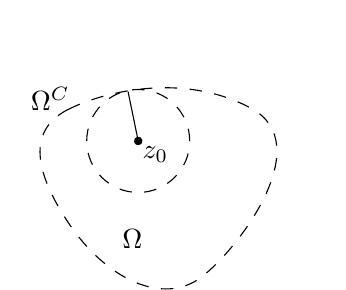
\begin{tikzpicture}[x=0.75pt,y=0.75pt,yscale=-0.45,xscale=0.45]
        %uncomment if require: \path (0,300); %set diagram left start at 0, and has height of 300
        
        %Shape: Polygon Curved [id:ds75764139255783] 
        \draw  [dash pattern={on 4.5pt off 4.5pt}] (105.36,58.25) .. controls (145.83,38.01) and (230.42,18.81) .. (301.26,57.26) .. controls (372.09,95.72) and (287.73,207.91) .. (247.26,238.26) .. controls (206.78,268.62) and (145.83,240.39) .. (105.36,179.68) .. controls (64.88,118.96) and (64.88,78.49) .. (105.36,58.25) -- cycle ;
        %Shape: Circle [id:dp1108533721802123] 
        \draw  [dash pattern={on 4.5pt off 4.5pt}] (125,92.13) .. controls (125,61.68) and (149.68,37) .. (180.13,37) .. controls (210.57,37) and (235.26,61.68) .. (235.26,92.13) .. controls (235.26,122.57) and (210.57,147.26) .. (180.13,147.26) .. controls (149.68,147.26) and (125,122.57) .. (125,92.13) -- cycle ;
        %Straight Lines [id:da9925386809993804] 
        \draw    (169.26,39.26) -- (180.13,92.13) ;
        \draw [shift={(180.13,92.13)}, rotate = 78.38] [color=black  ][fill=black  ][line width=0.75]      (0, 0) circle [x radius= 3.35, y radius= 3.35]   ;
        
        % Text Node
        \draw (160.38,184.08) node [anchor=north west][inner sep=0.75pt]    {$\Omega $};
        % Text Node
        \draw (62.38,32.08) node [anchor=north west][inner sep=0.75pt]    {$\Omega ^{C}$};
        % Text Node
        \draw (182.13,95.53) node [anchor=north west][inner sep=0.75pt]    {$z_{0}$};
        
        
        \end{tikzpicture}
        }

    Moreover, the radius of convergence is the radius of the largest open disk centered at $z_0$ upon which $f$ could be analytically continued.
\end{theorem}

\begin{proof}
    Let $r<\operatorname*{dist}(z_0,\reg^C)$ and $|z-z_0|\leq \rho<r$. Then \[f(z)=\frac{1}{2\pi i} \int_{{C_r(z_0)}}\frac{f(\zeta)\d \zeta}{\zeta-z}\] for all $|z-z_0|<\rho$. 

    As a function of $\zeta$, the series\sidenote{geometric series trick!} \[\frac{1}{\zeta-z}=\frac{1}{(\zeta-z_0)-(z-z_0)}=\frac{1}{\zeta-z_0}\cdot \frac{1}{1-\frac{z-z_0}{\zeta-z_0}}\]
    and so by geometric series formula:
    \begin{align*}
        \frac{1}{\zeta-z} &= \frac{1}{\zeta-z_0}\sum_{n=0}^{\infty}\left(\frac{z-z_0}{\zeta-z_0}\right)^n\\
        &= \sum_{n=0}^{\infty}\frac{(z-z_0)^n}{(\zeta-z_0)^{n+1}} &&\text{for } |z-z_0|\leq \rho
    \end{align*}
    converges uniformly on $|\zeta-z_0|=r$ by the Weierstrass M-test with $M_n=\left|\frac{z-z_0}{\zeta-z_0}\right|^n\leq \left(\frac{\rho}{r}\right)^n$.

    Thus, \begin{align*}
        f(z)&=\frac{1}{2\pi i}\int_{{C_r(z_0)}}\frac{f(\zeta)\d \zeta}{\zeta-z}\\
        &= \frac{1}{2\pi i}\int_{{C_r(z_0)}}\rt{\sum_{n=0}^{\infty}\frac{(z-z_0)^n}{(\zeta-z_0)^{n+1}}}\cdot f(\zeta)\d \zeta\\
        &= \sum_{n=0}^{\infty}(z-z_0)^n\bt{
            \frac{1}{2\pi i}\int_{{C_r(z_0)}}\frac{f(\zeta)\d \zeta}{(\zeta-z_0)^{n+1}}
        }
    \end{align*}
    And so we have our $\bt{\frac{f^{(n)}(z_0)}{n!}=a_n}$ in the highlighted part above. 
\end{proof}

\rmk Consequently, we also get Cauchy's theorem of derivatives: \[f^{(n)}(z_0) = \frac{n!}{2\pi i}\int_{{C_r(z_0)}}\frac{f(\zeta)\d \zeta}{(\zeta-z_0)^{n+1}}\]

\eg What is the radius of convergence for the power series of \[f(x)=\frac{e^{\sin x}+e^{-x^2}+x^2+7x^3}{\cos x}\] centered at $x_0=2$?

The theorem guarantees the existence of the power series, and the RoC would simply be the radius of which $f$ could be analytically continued. We observe that $f(x)$ cannot be defined when $\cos x=0$, i.e. $x=\frac{\pi}{2}$. Hence, the radius of convergence is just $2-\frac{\pi}{2}$ -- no need to compute \textit{any} derivatives or coefficients!

\spl

So now we have this result for computing the derivatives and integrals around a circle $C_r(z_0)$. Can we extend this to other closed curves of any shapes?

\[\begin{tikzpicture}[x=0.75pt,y=0.75pt,yscale=-1,xscale=1]
    %uncomment if require: \path (0,300); %set diagram left start at 0, and has height of 300
    
    %Curve Lines [id:da21494767258082992] 
    \draw    (202.26,132.76) .. controls (260.26,132.76) and (232.42,21.55) .. (303.26,60) .. controls (374.09,98.45) and (424.73,204.41) .. (384.26,234.76) .. controls (343.78,265.12) and (293.26,262.76) .. (245.26,241.76) .. controls (197.26,220.76) and (104.26,255.76) .. (80.26,215.76) .. controls (56.26,175.76) and (161.26,132.51) .. (202.26,132.76) -- cycle ;
    \draw [shift={(250.18,76.55)}, rotate = 112.47] [color=black  ][line width=0.75]    (10.93,-4.9) .. controls (6.95,-2.3) and (3.31,-0.67) .. (0,0) .. controls (3.31,0.67) and (6.95,2.3) .. (10.93,4.9)   ;
    \draw [shift={(380.72,140.93)}, rotate = 240.89] [color=black  ][line width=0.75]    (10.93,-4.9) .. controls (6.95,-2.3) and (3.31,-0.67) .. (0,0) .. controls (3.31,0.67) and (6.95,2.3) .. (10.93,4.9)   ;
    \draw [shift={(309.73,257.48)}, rotate = 0.74] [color=black  ][line width=0.75]    (10.93,-4.9) .. controls (6.95,-2.3) and (3.31,-0.67) .. (0,0) .. controls (3.31,0.67) and (6.95,2.3) .. (10.93,4.9)   ;
    \draw [shift={(153.76,235.89)}, rotate = 357.8] [color=black  ][line width=0.75]    (10.93,-4.9) .. controls (6.95,-2.3) and (3.31,-0.67) .. (0,0) .. controls (3.31,0.67) and (6.95,2.3) .. (10.93,4.9)   ;
    \draw [shift={(129.21,152.85)}, rotate = 153.94] [color=black  ][line width=0.75]    (10.93,-4.9) .. controls (6.95,-2.3) and (3.31,-0.67) .. (0,0) .. controls (3.31,0.67) and (6.95,2.3) .. (10.93,4.9)   ;
    %Shape: Arc [id:dp390751992975634] 
    \draw  [draw opacity=0] (365.61,148.43) .. controls (365.61,176.37) and (342.96,199.02) .. (315.02,199.02) .. controls (287.07,199.02) and (264.42,176.37) .. (264.42,148.43) .. controls (264.42,120.48) and (287.07,97.83) .. (315.02,97.83) .. controls (342.66,97.83) and (365.13,120.01) .. (365.6,147.54) -- (315.02,148.43) -- cycle ; \draw    (365.61,148.43) .. controls (365.61,176.37) and (342.96,199.02) .. (315.02,199.02) .. controls (287.07,199.02) and (264.42,176.37) .. (264.42,148.43) .. controls (264.42,120.48) and (287.07,97.83) .. (315.02,97.83) .. controls (342.11,97.83) and (364.23,119.13) .. (365.55,145.9) ; \draw [shift={(365.55,145.9)}, rotate = 89.02] [color=black  ][line width=0.75]    (10.93,-4.9) .. controls (6.95,-2.3) and (3.31,-0.67) .. (0,0) .. controls (3.31,0.67) and (6.95,2.3) .. (10.93,4.9)   ; 
    %Straight Lines [id:da7884227166046833] 
    \draw    (315.02,97.83) -- (315.02,148.43) ;
    \draw [shift={(315.02,148.43)}, rotate = 90] [color=black  ][fill=black  ][line width=0.75]      (0, 0) circle [x radius= 3.35, y radius= 3.35]   ;
    %Straight Lines [id:da21437723713367007] 
    \draw    (109.26,164) -- (267.26,164) ;
    %Straight Lines [id:da9640002297232435] 
    \draw    (363.26,163.86) -- (390.41,163.86) ;
    %Straight Lines [id:da7394620764040947] 
    \draw    (305,198) -- (305,257.26) ;
    %Straight Lines [id:da2656674999162538] 
    \draw    (304,60) -- (304,99.26) ;
    %Shape: Arc [id:dp7144254929573495] 
    \draw  [draw opacity=0] (232.12,221.17) .. controls (233.6,221.71) and (235.2,222) .. (236.87,222) .. controls (244.53,222) and (250.74,215.79) .. (250.74,208.13) .. controls (250.74,200.47) and (244.53,194.26) .. (236.87,194.26) .. controls (229.21,194.26) and (223,200.47) .. (223,208.13) .. controls (223,208.44) and (223.01,208.74) .. (223.03,209.05) -- (236.87,208.13) -- cycle ; \draw [color=cyan  ,draw opacity=1 ]   (234.05,221.71) .. controls (234.96,221.9) and (235.9,222) .. (236.87,222) .. controls (244.53,222) and (250.74,215.79) .. (250.74,208.13) .. controls (250.74,200.47) and (244.53,194.26) .. (236.87,194.26) .. controls (229.21,194.26) and (223,200.47) .. (223,208.13) .. controls (223,208.44) and (223.01,208.74) .. (223.03,209.05) ;  \draw [shift={(232.12,221.17)}, rotate = 355.35] [color=cyan  ,draw opacity=1 ][line width=0.75]    (10.93,-4.9) .. controls (6.95,-2.3) and (3.31,-0.67) .. (0,0) .. controls (3.31,0.67) and (6.95,2.3) .. (10.93,4.9)   ;
    
    % Text Node
    \draw (317.21,164.09) node [anchor=north west][inner sep=0.75pt]    {$z$};
    % Text Node
    \draw (303.95,117.47) node [anchor=north west][inner sep=0.75pt]    {$r$};
    
    
    \end{tikzpicture}
    \]
Same techniques! Hence, \[f^{(n)}(z) = \frac{n!}{2\pi i}\int_{\gamma}\frac{f(\zeta)\d \zeta}{(\zeta-z)^{n+1}}\] on any such closed curve $\gamma$.

\subsection{Liouville's theorem}
\begin{theorem}[Liouville's]
    A bounded entire function \sidenote{analytic on \(\C\)} is constant.
\end{theorem}
\begin{proof}
    Suppose $f$ is entire and $|f(z)|\leq M$ is bounded by $M$ for all $z\in \C$. Then \[f'(z)=\frac{1!}{2\pi i}\int_{C_R(z)}\frac{f(\zeta)}{(\zeta-z)^2}\d \zeta\] by Cauchy's integral formula. Hence, $|f'(z)|\leq \frac{1}{2\pi}\cdot \frac{M}{R^2}\cdot 2\pi R=\frac{M}{R}$ by the upper bound. Since $f$ is entire, there is no limit in what $R$ could be, so we let $R\to \infty$ and observe that $|f'(z)|=0$ for all $z\in \C$. Hence, $f'$ is identically 0, and so $f$ is constant.
\end{proof}

\noneg We know $|\cos x|\leq 1$ for all $x\in \R$, but $\cos z = \frac{e^{iz}+e^{-iz}}{2}$ is \textbf{not} bounded on $\C$. In fact, $\cos(-ix)=\frac{e^x+e^{-x}}{2}$ is unbounded for real $x$, so $\cos x$ is not bounded on the imaginary axis. Hence, we can't use Liouville's theorem here!

\subsection{Fundamental theorem of algebra}
\begin{theorem}[FToA]
    Every \textbf{nonconstant} complex polynomial has a zero in $\C$.\sidenote{recall ``$\C$ is an algebraically closed field''}
\end{theorem}
\begin{proof}
    Suppose towards a contradiction that $p$ is a \textbf{nonconstant} polynomial over $\C$ with no zeros in $\C$. Then $f=\frac{1}{p}$ is an entire function because we never divide by 0. Recall HW2 Ex2 showed that $\lim_{|z|\to \infty}p(z)=\infty$. That is, for any $M>0$, there exists $R>0$ such that whenever $|z|>R$, we have $|p(z)|>M$.

    Thus, $\lim_{|z|\to \infty}f(z) =  \lim_{|z|\to \infty}\frac{1}{p(z)}=0$. In particular, we can find a $R>0$ such that whenever $|z|>R$, we have \dashuline{$|f(z)|<1$ is bounded outside of the circle $|z|=R$}. Since the closed disk $|z|\leq R$ is compact and $f$ is continuous, \dashuline{$f$ is bounded inside this closed disk $|z|\leq R$.}\sidenote{Extreme value theorem}

    Hence, $f$ is a bounded entire function, meaning that it is constant by Liouville's theorem, and hence $p$ is \textbf{constant} too. This cause a contradiction.
\end{proof}

\subsection{Zeros of analytic functions}
Recall the analytic functions are infinitely differentiable.

Suppose $f:\reg\to\C$ is analytic and $f(z_0)=0$ for some $z_0\in \reg$, and $f$ is not identically 0 on an open neighbourhood of $z_0$. Then \[f(z)=\sum_{j=n}^{\infty}a_j(z-z_0)^j\] for some $n\geq 1$ such that $a_n\neq 0$\sidenote{the lowest power term that has a nonzero coefficient, and also $n$ is the order of the zero $z_0$.}. Hence: \begin{align*}
    f(z)&=\sum_{j=n}^{\infty}a_j(z-z_0)^j\\
    &= (z-z_0)^n \sum_{j=n}^{\infty}a_j(z-z_0)^{j-n}\\
    &= (z-z_0)^n \rt{\sum_{k=0}^{\infty}a_{n+k}(z-z_0)^k}
\end{align*}
let $g(z)=\rt{\sum_{k=0}^{\infty}a_{n+k}(z-z_0)^k}$. Observe that $g$ is analytic and $g(z_0)=a_n\neq 0$. This and the continuity of $g$ at $z_0$ ensures that $g$ is nonzero on some open disk $|z-z_0|<\delta$. Therefore, $f(z)=(z-z_0)^n\rt{g(z)}$ does not vanish on $0<|z-z_0|<\delta$.

\rmk The zeros of $f$ are \textbf{isolated} in $\reg$. That is, we can't have a sequence of zeros of $f$ converging to some $z_0\in \reg$, as then we can't find a nonzero disk around $z_0$!

\begin{theorem}
    If $f:\reg\to\C$ is analytic and not identically zero, then each zero of $f$ is isolated and has finite order. 
\end{theorem}
\begin{proof}
    Assume BWOC that the zeros are not isolated.

    By definition, $\reg$ is connected. By definition$\times 2$, a subset $S\subseteq\reg$ is \textbf{clopen} if it is open and closed as a subset of $\reg$. \sidenote{Example of nontrivial clopen subsets: \[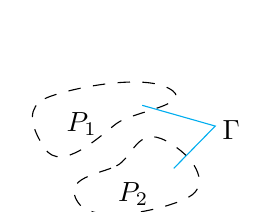
\begin{tikzpicture}[x=0.75pt,y=0.75pt,yscale=-0.4,xscale=0.4]
        %uncomment if require: \path (0,300); %set diagram left start at 0, and has height of 300
        
        %Shape: Polygon Curved [id:ds3275739299185525] 
        \draw  [dash pattern={on 4.5pt off 4.5pt}] (113,73.24) .. controls (133,63.24) and (227.26,41.75) .. (262.26,60.75) .. controls (297.26,79.75) and (219.26,88.26) .. (199.26,103.26) .. controls (179.26,118.26) and (133,163.24) .. (113,133.24) .. controls (93,103.24) and (93,83.24) .. (113,73.24) -- cycle ;
        %Shape: Polygon Curved [id:ds29563927191425465] 
        \draw  [dash pattern={on 4.5pt off 4.5pt}] (199.26,154.26) .. controls (219.26,144.26) and (224.26,105.26) .. (259.26,124.26) .. controls (294.26,143.26) and (310.26,174.26) .. (290.26,189.26) .. controls (270.26,204.26) and (173,228.24) .. (153,198.24) .. controls (133,168.24) and (179.26,164.26) .. (199.26,154.26) -- cycle ;
        %Straight Lines [id:da6767121224748709] 
        \draw [color=cyan  ,draw opacity=1 ]   (268.26,157.26) -- (318.26,106.26) -- (230.26,81.26) ;
        
        % Text Node
        \draw (136,86.4) node [anchor=north west][inner sep=0.75pt]    {$P_{1}$};
        % Text Node
        \draw (198,171.4) node [anchor=north west][inner sep=0.75pt]    {$P_{2}$};
        % Text Node
        \draw (324,96.4) node [anchor=north west][inner sep=0.75pt]    {$\Gamma $};
        
        
        \end{tikzpicture}
        \]In this $\Gamma$ (NOT a region), the clopen subsets are $P_1,P_2,\emptyset,\Gamma$.}
    In a connected region $\reg$, only $\emptyset, \reg$ are clopen.

    Let $S=\{z\in \reg : f^{(j)}(z)=0 \quad \forall\, j=0,1,2,\dots\}$. If $z_0\in S$ then $f$ is zero on some open disk centered at $z_0$. \dashuline{Hence, $S$ is open!}

    Now suppose $w$ is a limit of a sequence in $S$. Since $f$ is continuous, $f^{(j)}$ is continuous for all $j\in \N$. This enruses that $f^{(j)}(w)=0$. \dashuline{Thus, $S$ is closed!}

    Therefore, $S$ is clopen in $\reg$, so either $S$ is the empty set or $S=\reg$. If $S=\reg$, then $f$ is the zero function, so that cannot happen! Therefore, $S=\emptyset$, and so we don't have a cluster of zeros.
\end{proof}

\corollary If $f$ is a nonconstant analytic function, its zero set is \textbf{countable}. This is because within an open region, we can have at most countably infinite number of disjoint open sets. We let these open sets be $f^{-1}(\{0\})$.

\subsection{Identity theorem}
\defn An \textbf{accumulation} point of $S$ is a point that is the limit of a sequence of \textbf{distinct} points of $S$.
\[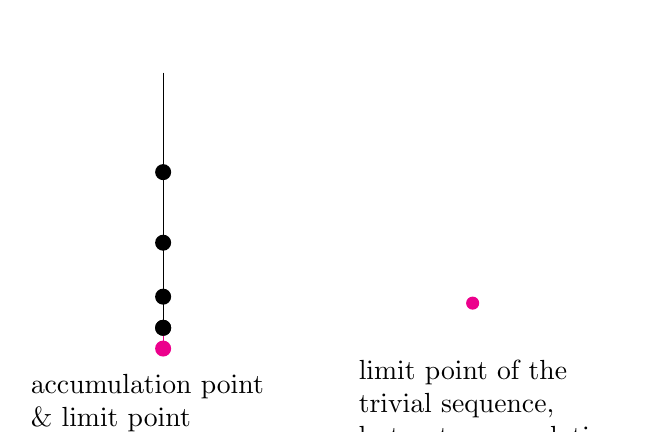
\begin{tikzpicture}[x=0.75pt,y=0.75pt,yscale=-1,xscale=1]
    %uncomment if require: \path (0,300); %set diagram left start at 0, and has height of 300
    
    %Straight Lines [id:da556992577885977] 
    \draw    (100,105.76) -- (100,139.76) ;
    \draw [shift={(100,139.76)}, rotate = 90] [color=black  ][fill=black  ][line width=0.75]      (0, 0) circle [x radius= 3.35, y radius= 3.35]   ;
    %Straight Lines [id:da08524159729103475] 
    \draw    (100,57.76) -- (100,105.76) ;
    \draw [shift={(100,105.76)}, rotate = 90] [color=black  ][fill=black  ][line width=0.75]      (0, 0) circle [x radius= 3.35, y radius= 3.35]   ;
    %Straight Lines [id:da41449224969428156] 
    \draw    (100,139.76) -- (100,165.76) ;
    \draw [shift={(100,165.76)}, rotate = 90] [color=black  ][fill=black  ][line width=0.75]      (0, 0) circle [x radius= 3.35, y radius= 3.35]   ;
    %Straight Lines [id:da4533906108237473] 
    \draw    (100,165.76) -- (100,180.76) ;
    \draw [shift={(100,180.76)}, rotate = 90] [color=black  ][fill=black  ][line width=0.75]      (0, 0) circle [x radius= 3.35, y radius= 3.35]   ;
    %Straight Lines [id:da15251507183156088] 
    \draw [color=magenta  ,draw opacity=1 ]   (100,180.76) -- (100,190.76) ;
    \draw [shift={(100,190.76)}, rotate = 90] [color=magenta  ,draw opacity=1 ][fill=magenta  ,fill opacity=1 ][line width=0.75]      (0, 0) circle [x radius= 3.35, y radius= 3.35]   ;
    %Straight Lines [id:da447461872834491] 
    \draw    (100,165.76) -- (100,180.76) ;
    \draw [shift={(100,180.76)}, rotate = 90] [color=black  ][fill=black  ][line width=0.75]      (0, 0) circle [x radius= 3.35, y radius= 3.35]   ;
    %Shape: Circle [id:dp7661245715545606] 
    \draw  [color=magenta  ,draw opacity=1 ][fill=magenta  ,fill opacity=1 ] (252,168.87) .. controls (252,167.29) and (250.71,166) .. (249.13,166) .. controls (247.54,166) and (246.26,167.29) .. (246.26,168.87) .. controls (246.26,170.46) and (247.54,171.74) .. (249.13,171.74) .. controls (250.71,171.74) and (252,170.46) .. (252,168.87) -- cycle ;
    
    % Text Node
    \draw (35,202) node [anchor=north west][inner sep=0.75pt]   [align=left] {accumulation point \\\& limit point};
    % Text Node
    \draw (193,195) node [anchor=north west][inner sep=0.75pt]   [align=left] {limit point of the \\trivial sequence, \\but not accumulation};
    
    
    \end{tikzpicture}
    \]

\begin{theorem}
    Let $f,g:\reg\to \C$ be analytic. If $f=g$ on a subset of $\reg$ that has an accumulation point in $\reg$, then $f=g$ on the entire $\reg$.
\end{theorem}
\begin{proof}
    If the zero set of $f-g$ has an accumulation point in $\reg$, then $f-g$ has a zero that is not isolated (no open disk around it since some zeros keep converging to that accumulation point), so $f-g$ is identically zero on $\reg$.
\end{proof}

\eg There is only one way to extend $\cos x, \sin x, \exp x$ from $\R$ to $\C$ because two entire functions that agree on $\R$ agree on $\C$. 

\eg Similarly, there is also only one way to get an analytic continuation of the Riemann zeta function to $\re s>0$. 

\subsection{Maximum modulus principle}
Recall this handwavy physics application \hyperlink{physics}{here}. We now have a more rigorous way to state this!\sidenote{Not exactly equivalent, though.}

\begin{theorem}[Maximum modulus principle]
    Let $f$ be analytic on a region $\reg$ that contains a piecewise $C'$ simple closed curve $\gamma$ and its interior. Then \[|f(z)|\leq \max_{\zeta\in \gamma}|f(\zeta)|\] for all $z$ in the interior of $\gamma$.
\end{theorem}
\begin{proof}
    Let $M= \max_{\zeta\in \gamma}|f(\zeta)|$. Fix $z$ inside $\gamma$. Let $L$ denote the length of $\gamma$ and let $r=\inf_{\zeta\in \gamma}|z-\zeta$, which is positive (so $z$ isn't arbitrarily close to $\gamma$). 

    Apply Cauchy's integral formula to the $n$-th power of $f$: \[f(z)^n = \frac{1}{2\pi i}\int_{\gamma}\frac{f(\zeta)^n\d\zeta}{\zeta-z}\]
    Thus, \[|f(z)|^n \leq \frac{1}{2\pi}\cdot \frac{M^n}{r}L\]
    Now we just take the $n$-th root everywhere:\[|f(z)|\leq M\left(\frac{L}{2\pi r}\right)^{1/n}\] We use arbitrarily large $n$ and get $|f(z)|\leq M$.
\end{proof}

\subsection{Schwarz' lemma}
\begin{lemma}[Schwarz']
    Let $f:\D\to \D^-$ be analytic and $f(0)=0$. Then: \begin{enumerate}[label=(\alph*)]
        \item \(|f'(0)|\leq 1\) and $|f(z)|\leq |z|$ for all $z\in \D$.
        \item If $|f'(0)|=1$ or $|f(z_0)|=|z_0|$ for some $z_0\neq 0$, then $f(z)=\lambda z$ for some $\lambda$ with $|\lambda|=1$.
    \end{enumerate}
\end{lemma}

\begin{proof}[Proof part (a)]
    Since $f(0)=0$, we have that the constant term of $f$ is 0, and so $f(z)=zg(z)$ for some $g$ analytic on $\D$. Thus, \[f'(z)=g(z)+zg'(z)\] and hence $f'(0)=g(0)$. Hence, \[g(z)=\begin{cases}
        \frac{f(z)}{z} & z\neq 0\\
        f'(0) &z=0
    \end{cases}\]
    If $|z|\leq r<1$, then by the maximum modulus principle, \begin{align*}
        |g(z)|&\leq \max_{|\zeta|=r}|g(\zeta)|\\
        &= \max_{|\zeta|=r}\left|\frac{f(\zeta)}{\zeta}\right|\\
        &\leq \frac{1}{r} &\text{since }f:\D\to\D^-
    \end{align*}
    Let $r\to 1^-$ and get $|g(z)|\leq 1$ for all $z\in \D$, which is the (a) part of our result.
\end{proof}

\begin{proof}[Proof part (b)]
    Maximum modulus principle says the given conditions imply $g$ is constant. The constant $\lambda$ has absolute value 1, so $\frac{f(z)}{z}=\lambda$ and so $f(z)=\lambda z$.
\end{proof}

\subsection{Automorphism group of a region}
\defn Let $\reg$ be a region in $\C$. We let the automorphism group of the region \(\Aut (\Omega)\) be the set of all \textbf{bijective analytic functions} from $\reg$ to $\reg$.
\begin{itemize}
    \item \(\Aut (\Omega)\) contains the identity function $f(z)=z$.
    \item \(\Aut (\Omega)\) is closed under composition.\sidenote{And composition is a binary operation with associativity}
    \item \(\Aut (\Omega)\) is closed under inverses: if $f:\reg\to\reg$ is an analytic bijection, then $\inv{f}:\reg\to \reg$ exists and is \textbf{analytic}.
    \rmk There appears to be a `counterexample': \[\begin{tikzpicture}[x=0.75pt,y=0.75pt,yscale=-1,xscale=1]
        %uncomment if require: \path (0,300); %set diagram left start at 0, and has height of 300
        
        %Shape: Polynomial [id:dp016145053242946572] 
        \draw   (45,211) .. controls (92.42,73.82) and (139.84,213.69) .. (187.26,76.51) ;
        %Shape: Axis 2D [id:dp40514861748695963] 
        \draw  (37,143.51) -- (204.26,143.51)(119.26,54) -- (119.26,224.51) (197.26,138.51) -- (204.26,143.51) -- (197.26,148.51) (114.26,61) -- (119.26,54) -- (124.26,61)  ;
        %Shape: Axis 2D [id:dp23339690918753542] 
        \draw  (278,143.51) -- (445.26,143.51)(360.26,54) -- (360.26,224.51) (438.26,138.51) -- (445.26,143.51) -- (438.26,148.51) (355.26,61) -- (360.26,54) -- (365.26,61)  ;
        %Shape: Polynomial [id:dp9729500065216796] 
        \draw   (425.26,74.5) .. controls (292.77,120.29) and (427.85,166.09) .. (295.37,211.88) ;
        %Straight Lines [id:da8672984437837188] 
        \draw [color=magenta  ,draw opacity=1 ]   (360.26,143.51) -- (398.91,186.03) ;
        \draw [shift={(400.26,187.51)}, rotate = 227.73] [color=magenta  ,draw opacity=1 ][line width=0.75]    (10.93,-3.29) .. controls (6.95,-1.4) and (3.31,-0.3) .. (0,0) .. controls (3.31,0.3) and (6.95,1.4) .. (10.93,3.29)   ;
        \draw [shift={(360.26,143.51)}, rotate = 47.73] [color=magenta  ,draw opacity=1 ][fill=magenta  ,fill opacity=1 ][line width=0.75]      (0, 0) circle [x radius= 3.35, y radius= 3.35]   ;
        
        % Text Node
        \draw (162,55.4) node [anchor=north west][inner sep=0.75pt]    {$x^{3}$};
        % Text Node
        \draw (433,46.4) node [anchor=north west][inner sep=0.75pt]    {$x^{1/3}$};
        % Text Node
        \draw (376,194) node [anchor=north west][inner sep=0.75pt]  [color=magenta  ,opacity=1 ] [align=left] {not differentiable?};
        
        
        \end{tikzpicture}
        \]
        However, this is only true in $\R$. In $\C$, we observe that $z^3$ is \textbf{not} a bijection at $0$, so this function is not in the group at all!
\end{itemize}

\addlink{Riemann Mapping Theorem}
\begin{theorem}[Riemann Mapping]
    If $\reg$ is simply connected (no holes)\sidenote{Except for the entire $\C$, which has only constant functions if bounded (by Liouville thm).}, then it could be conformally mapped to a disk.
    \drawing{0.5\linewidth}{image-7.png}
\end{theorem}

\spl

Recall from HW1 that for each $w\in \D$, we have a bijection \[\phi_w(z)=\frac{-z+w}{-\bar w z+1}\] from $\D$ to $\D$ and $\phi\circ \phi=\mathrm{id}$. To see this, observe the matrix representation \[\begin{bmatrix}
    -1 & w\\ -\bar w & 1
\end{bmatrix}\cdot \begin{bmatrix}
    -1 & w\\ -\bar w & 1
\end{bmatrix} = \begin{bmatrix}
    1-|w|^2 & 0 \\ 0 &  1-|w|^2
\end{bmatrix}\sim I\]
Furthermore, note $\phi_w(0)=w$. Suppose $f\in \Aut(\D)$, then there is a unique $w\in \D$ such that $f(w)=0$. Define $g=f\circ \phi_w\in \Aut(\D)$. Note that $g(0)=f(\phi_w(0))=f(w)=0$. By Schwarz' lemma, we have \rt{$|g(z)|\leq |z|$} for all $z\in \D$. 

Since $\inv g\in \Aut(\D)$, we also have $|\inv g(z)|\leq |z|$ for all $z\in \D$. Now substitute $g(z)$ for $z$ since it's also in the disk. Hence, \bt{$|z|=|\inv g (g(z))|\leq |g(z)|$}. Therefore, we are forced to conclude that $\textcolor{violet}{|z|=|g(z)|}$ for ALL $z\in \D$!

Since $\textcolor{violet}{|z|=|g(z)|}$ for ALL $z\in \D$, Schwarz' lemma says $g(z)=\lambda z$ for some $|\lambda|=1$. Let $\lambda=e^{i\theta}$ for some $\theta\in \R$. Thus, \[g(z)=f(\phi_w(z))=e^{i\theta}z\]
and so \[e^{i\theta}\phi_w(z)=f(\phi_w(\phi_w(z)))=f(z)\]
since $\phi_w\circ \phi_w=\mathrm{id}$. Therefore, $\displaystyle f(z)=e^{i\theta}\frac{w-z}{1-\bar wz}$.

Therefore, 
\begin{proposition}
    \[\Aut (\D)= \left\{e^{i\theta}\frac{w-z}{1-\bar wz}\; \Bigg \vert\; \theta\in [0,2\pi), w\in \D\right\}\]
\end{proposition}

\rmk The topological representation of the automorphism group of $\D$ is a `skinless torus' (collection of open disks revolving from 0 to $2\pi$).

\subsection{Morera's theorem}
\begin{theorem}[Morera]
    If $f:\reg\to\C$ is continuous and $\int_{\gamma}f(\zeta)\d\zeta=0$ for all \underline{\hspace{2cm}} $\gamma$ in $\reg$, then $f$ is analytic on $\reg$. \sidenote{the blank can be `rectangles', `triangles', `piecewise $C^1$ closed curves', etc.}
\end{theorem}
\begin{proof}[Proof see \href{https://stephangarcia.sites.pomona.edu/teaching/24S-135/Lecture/24S-135-Lecture16.pdf}{notes}]
\end{proof}

\subsection{Weierstrass convergence theorem}
Let $f_n(z)$ be analytic for every $n\in \N$. We are still not sure that $\sum_{n=1}^{\infty} f_n(z)$ is analytic yet!

\begin{theorem}[Weierstrass convergence]
    If $f_n:\reg\to \C$ are analytic and $f_n$ converges \textit{locally uniformly} on $\reg$ to the limit function $f$ (\bt{$\Leftrightarrow$ uniform convergence on compact sets}), then \textcolor{darkgray}{$f$ is analytic and for each fixed $m$, $f_n^{m}$ converges to $f^{(m)}$ locally uniformly on $\reg$ and $f$ is infinitely differentiable}. 
\end{theorem}

\rmk This is a huge contrast with the\textit{ Weierstrass approximation theorem} in real analysis, which says that \textcolor{darkgray}{if $f:[0,1]\to \R$, then there is a sequence of polynomials $p_n$ such that $p_n$ converges to $f$ uniformly on $[0,1]$}. That is, even the most pathological, nowhere-differentiable functions in $\R$ are a limit of some polynomial sequences! However, in the $\C$ world, the limit of any analytic function is still analytic.

\section{Laurent series \& isolated singularities}
Sometimes the domain $\reg$ isn't the largest domain where an analytic function can be analytic. So far, we know we can find the largest disk centered at a point in $\reg$\sidenote{the disk could exceed the bounds of $\reg$!} in which a function is analytic and the power series exists there:\[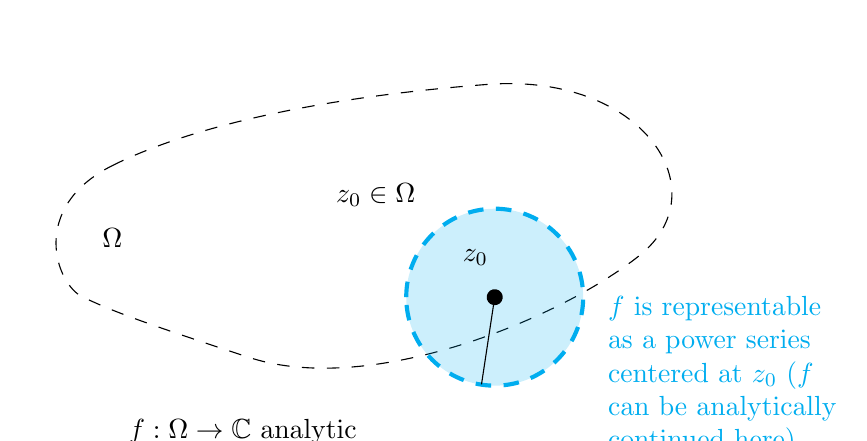
\begin{tikzpicture}[x=0.75pt,y=0.75pt,yscale=-1,xscale=1]
    %uncomment if require: \path (0,300); %set diagram left start at 0, and has height of 300
    
    %Shape: Polygon Curved [id:ds40363339954426203] 
    \draw  [dash pattern={on 4.5pt off 4.5pt}] (105.36,58.25) .. controls (145.83,38.01) and (210.86,24.86) .. (286.14,19.12) .. controls (361.42,13.38) and (398.26,70.64) .. (359.26,101.64) .. controls (320.26,132.64) and (229.26,169.64) .. (171.26,150.64) .. controls (113.26,131.64) and (104.26,127.64) .. (91.26,121.64) .. controls (78.26,115.64) and (64.88,78.49) .. (105.36,58.25) -- cycle ;
    %Shape: Circle [id:dp18109739983497897] 
    \draw  [color=cyan  ,draw opacity=1 ][fill=cyan  ,fill opacity=0.2 ][dash pattern={on 5.63pt off 4.5pt}][line width=1.5]  (247,121.63) .. controls (247,98.09) and (266.09,79) .. (289.63,79) .. controls (313.17,79) and (332.26,98.09) .. (332.26,121.63) .. controls (332.26,145.17) and (313.17,164.26) .. (289.63,164.26) .. controls (266.09,164.26) and (247,145.17) .. (247,121.63) -- cycle ;
    %Straight Lines [id:da39916826624746937] 
    \draw    (289.63,121.63) -- (283.26,163.64) ;
    \draw [shift={(289.63,121.63)}, rotate = 98.62] [color=black  ][fill=black  ][line width=0.75]      (0, 0) circle [x radius= 3.35, y radius= 3.35]   ;
    
    % Text Node
    \draw (99.38,87.08) node [anchor=north west][inner sep=0.75pt]    {$\Omega $};
    % Text Node
    \draw (273,97.4) node [anchor=north west][inner sep=0.75pt]    {$z_{0}$};
    % Text Node
    \draw (343,120) node [anchor=north west][inner sep=0.75pt]  [color=cyan  ,opacity=1 ] [align=left] {$\displaystyle f$ is representable\\as a power series \\centered at $\displaystyle z_{0}$ ($\displaystyle f$ \\can be analytically\\continued here)};
    % Text Node
    \draw (212,65.4) node [anchor=north west][inner sep=0.75pt]    {$z_{0} \in \Omega $};
    % Text Node
    \draw (112,179) node [anchor=north west][inner sep=0.75pt]   [align=left] {$\displaystyle f:\Omega \rightarrow \mathbb{C}$ analytic};
    
    
    \end{tikzpicture}\]

Can we do even better than that?

\subsection{Laurent series}
\eg Let $f(z)=\frac{1}{z(z-1)}$ analytic on $\C\backslash\{0,1\}$. We realize that if we restrict $0<|z|<1$, then \[f(z)=\frac{-1}{z}\cdot\frac{1}{1-z}=\frac{-1}{z}-1-z-z^2-\dots\] 
is the \textbf{Laurent series} of $f(z)$ centered at 0, a point where $f(z)$ isn't even defined!

\eg We continue with the previous function. This time, we restrict $|z|>1$ and express it as:\[f(z)=\frac{1}{z^2(1-\frac{1}{z})} = \frac{1}{z^2}+\frac{1}{z^3}+\dots\]

Hence, we now have different series for $f$ in different regions: \[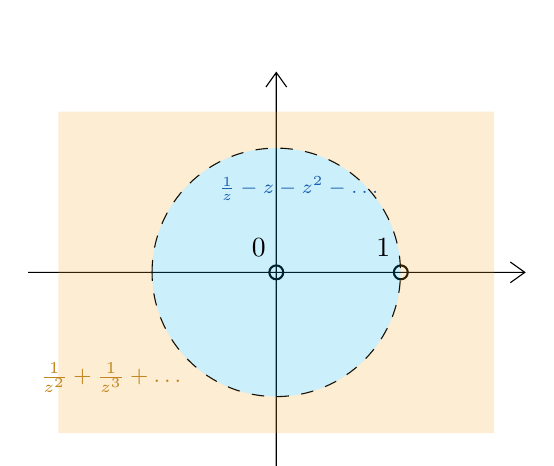
\begin{tikzpicture}[x=0.75pt,y=0.75pt,yscale=-1,xscale=1]
    %uncomment if require: \path (0,300); %set diagram left start at 0, and has height of 300
    
    %Shape: Axis 2D [id:dp8096713031018239] 
    \draw  (60.49,170) -- (299.74,170)(180,73.71) -- (180,270.86) (292.74,165) -- (299.74,170) -- (292.74,175) (175,80.71) -- (180,73.71) -- (185,80.71)  ;
    %Straight Lines [id:da8307990020001665] 
    \draw    (182.35,170) -- (237.65,170) ;
    \draw [shift={(240,170)}, rotate = 0] [color=black  ][line width=0.75]      (0, 0) circle [x radius= 3.35, y radius= 3.35]   ;
    \draw [shift={(180,170)}, rotate = 0] [color=black  ][line width=0.75]      (0, 0) circle [x radius= 3.35, y radius= 3.35]   ;
    %Shape: Circle [id:dp6485221177915352] 
    \draw  [fill=cyan  ,fill opacity=0.2 ][dash pattern={on 4.5pt off 4.5pt}] (120.14,170) .. controls (120.14,136.94) and (146.94,110.14) .. (180,110.14) .. controls (213.06,110.14) and (239.86,136.94) .. (239.86,170) .. controls (239.86,203.06) and (213.06,229.86) .. (180,229.86) .. controls (146.94,229.86) and (120.14,203.06) .. (120.14,170) -- cycle ;
    %Shape: Path Data [id:dp866707860246108] 
    \draw  [draw opacity=0][fill={rgb, 255:red, 245; green, 166; blue, 35 }  ,fill opacity=0.2 ][dash pattern={on 4.5pt off 4.5pt}] (180,110.14) .. controls (213.06,110.14) and (239.86,136.94) .. (239.86,170) .. controls (239.86,203.06) and (213.06,229.86) .. (180,229.86) .. controls (146.94,229.86) and (120.14,203.06) .. (120.14,170) .. controls (120.14,136.94) and (146.94,110.14) .. (180,110.14) -- cycle (75,92.5) -- (75,247.5) -- (285,247.5) -- (285,92.5) -- (75,92.5) -- cycle ;
    
    % Text Node
    \draw (167,152.4) node [anchor=north west][inner sep=0.75pt]    {$0$};
    % Text Node
    \draw (227,152.4) node [anchor=north west][inner sep=0.75pt]    {$1$};
    % Text Node
    \draw (151,122.4) node [anchor=north west][inner sep=0.75pt]  [font=\scriptsize,color={rgb, 255:red, 25; green, 96; blue, 175 }  ,opacity=1 ]  {$\frac{1}{z} -z-z^{2} -\dotsc $};
    % Text Node
    \draw (65,212.4) node [anchor=north west][inner sep=0.75pt]  [font=\footnotesize,color={rgb, 255:red, 194; green, 132; blue, 28 }  ,opacity=1 ]  {$\frac{1}{z^{2}} +\frac{1}{z^{3}} +\dotsc $};
    
    
    \end{tikzpicture}
    \]

\defn[Laurent series] A series in the form $\displaystyle \sum_{\rt{n=-\infty}}^{\infty}a_n(z-z_0)^n$ is a \textbf{Laurent series}. It converges at $z\in \C$ if \textbf{both} the \uline{analytic part} \(\displaystyle \sum_{\rt{n=0}}^{\infty}a_n(z-z_0)^n\) and the \uline{principal part} \(\displaystyle \sum_{n=1}^{\infty}a_{\bt{-n}}(z-z_0)^{\bt{-n}}\) converge at $z$. If this occurs, the Laurent series would be \[\sum_{\rt{n=-\infty}}^{\infty}a_n(z-z_0)^n = \sum_{\rt{n=0}}^{\infty}a_n(z-z_0)^n +\sum_{n=1}^{\infty}a_{\bt{-n}}(z-z_0)^{\bt{-n}}\] and also converges.

\lemma Recall that if $n\neq -1$, then $\frac{(z-z_0)^{n+1}}{n+1}$ is an antiderivative of $(z-z_0)^n$ on $\C$. \textbf{So} if $\gamma$ is simple closed, then by FTC, \[\frac{1}{2\pi i}\int_{\gamma}(z-z_0)^n\d z=0\] whenever $n\neq 1$. In addition, by Cauchy's integral formula, $\frac{1}{2\pi i}\int_{\gamma}\frac{\d z}{z-z_0}=1$. Therefore, if $z_0$ is in the interior of a simple closed curve $\gamma$, then \[\frac{1}{2\pi i}\int_{\gamma}(z-z_0)^n\d z= \begin{cases}
    0 & n\neq -1\\
    1 & n=-1
\end{cases}\]

\begin{proof}
    We previously know the result above when $\gamma$ is a circle. We now extend it to all simple closed curves by a familiar trick as follows:
    \[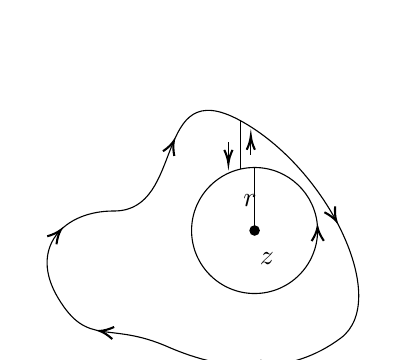
\begin{tikzpicture}[x=0.75pt,y=0.75pt,yscale=-.6,xscale=.6]
        %uncomment if require: \path (0,300); %set diagram left start at 0, and has height of 300
        
        %Curve Lines [id:da7016804119762063] 
        \draw    (150.26,97.76) .. controls (208.26,97.76) and (180.42,-13.45) .. (251.26,25) .. controls (322.09,63.45) and (372.73,169.41) .. (332.26,199.76) .. controls (291.78,230.12) and (241.26,227.76) .. (193.26,206.76) .. controls (145.26,185.76) and (129.26,207.64) .. (105.26,167.64) .. controls (81.26,127.64) and (109.26,97.51) .. (150.26,97.76) -- cycle ;
        \draw [shift={(198.18,41.55)}, rotate = 112.47] [color=black  ][line width=0.75]    (10.93,-4.9) .. controls (6.95,-2.3) and (3.31,-0.67) .. (0,0) .. controls (3.31,0.67) and (6.95,2.3) .. (10.93,4.9)   ;
        \draw [shift={(328.72,105.93)}, rotate = 240.89] [color=black  ][line width=0.75]    (10.93,-4.9) .. controls (6.95,-2.3) and (3.31,-0.67) .. (0,0) .. controls (3.31,0.67) and (6.95,2.3) .. (10.93,4.9)   ;
        \draw [shift={(257.73,222.48)}, rotate = 0.74] [color=black  ][line width=0.75]    (10.93,-4.9) .. controls (6.95,-2.3) and (3.31,-0.67) .. (0,0) .. controls (3.31,0.67) and (6.95,2.3) .. (10.93,4.9)   ;
        \draw [shift={(138.71,194.06)}, rotate = 8.82] [color=black  ][line width=0.75]    (10.93,-4.9) .. controls (6.95,-2.3) and (3.31,-0.67) .. (0,0) .. controls (3.31,0.67) and (6.95,2.3) .. (10.93,4.9)   ;
        \draw [shift={(107.34,112.99)}, rotate = 130.63] [color=black  ][line width=0.75]    (10.93,-4.9) .. controls (6.95,-2.3) and (3.31,-0.67) .. (0,0) .. controls (3.31,0.67) and (6.95,2.3) .. (10.93,4.9)   ;
        %Shape: Arc [id:dp13815379083723078] 
        \draw  [draw opacity=0] (313.61,113.43) .. controls (313.61,113.43) and (313.61,113.43) .. (313.61,113.43) .. controls (313.61,141.37) and (290.96,164.02) .. (263.02,164.02) .. controls (235.07,164.02) and (212.42,141.37) .. (212.42,113.43) .. controls (212.42,85.48) and (235.07,62.83) .. (263.02,62.83) .. controls (290.66,62.83) and (313.13,85.01) .. (313.6,112.54) -- (263.02,113.43) -- cycle ; \draw    (313.61,113.43) .. controls (313.61,113.43) and (313.61,113.43) .. (313.61,113.43) .. controls (313.61,141.37) and (290.96,164.02) .. (263.02,164.02) .. controls (235.07,164.02) and (212.42,141.37) .. (212.42,113.43) .. controls (212.42,85.48) and (235.07,62.83) .. (263.02,62.83) .. controls (290.11,62.83) and (312.23,84.13) .. (313.55,110.9) ; \draw [shift={(313.55,110.9)}, rotate = 89.02] [color=black  ][line width=0.75]    (10.93,-4.9) .. controls (6.95,-2.3) and (3.31,-0.67) .. (0,0) .. controls (3.31,0.67) and (6.95,2.3) .. (10.93,4.9)   ; 
        %Straight Lines [id:da8914465255998514] 
        \draw    (263.02,62.83) -- (263.02,113.43) ;
        \draw [shift={(263.02,113.43)}, rotate = 90] [color=black  ][fill=black  ][line width=0.75]      (0, 0) circle [x radius= 3.35, y radius= 3.35]   ;
        %Straight Lines [id:da9471588673663345] 
        \draw    (252,25) -- (252,64.26) ;
        %Straight Lines [id:da9805830469698456] 
        \draw    (242,42.64) -- (242,57.64) ;
        \draw [shift={(242,59.64)}, rotate = 270] [color=black  ][line width=0.75]    (10.93,-3.29) .. controls (6.95,-1.4) and (3.31,-0.3) .. (0,0) .. controls (3.31,0.3) and (6.95,1.4) .. (10.93,3.29)   ;
        %Straight Lines [id:da036041464758245434] 
        \draw    (260,52.64) -- (260,39.64) ;
        \draw [shift={(260,37.64)}, rotate = 90] [color=black  ][line width=0.75]    (10.93,-3.29) .. controls (6.95,-1.4) and (3.31,-0.3) .. (0,0) .. controls (3.31,0.3) and (6.95,1.4) .. (10.93,3.29)   ;
        
        % Text Node
        \draw (265.21,129.09) node [anchor=north west][inner sep=0.75pt]    {$z$};
        % Text Node
        \draw (251.95,82.47) node [anchor=north west][inner sep=0.75pt]    {$r$};
        
        
        \end{tikzpicture}
        \]
\end{proof}

\subsubsection{Laurent expansion theorem}
\theorem[Laurent expansion] Suppose $f$ is analytic on the annular region $A=\{z\in \C\mid R_1<|z-z_0|<R_2\}$.\sidenote{$R_1=0,R_2=\infty$ are okay} Then $f$ has a locally uniformly convergent Laurent expansion $$
f(z)=\sum_{n=-\infty}^{\infty} a_n\left(z-z_0\right)^n
$$
on $A$. Moreover, the Laurent coefficients are
$$
a_n=\frac{1}{2 \pi i} \int_{C_r\left(z_0\right)} \frac{f(\zeta) d \zeta}{\left(\zeta-z_0\right)^{n+1}}
$$
for any $r$ such that $R_1<r<R_2$.

\begin{proof}[Proof gist]
    For a gist of why this works:\sidenote{For rigorous proof, see \href{https://stephangarcia.sites.pomona.edu/teaching/24S-135/Lecture/24S-135-Lecture17.pdf}{notes}.} \[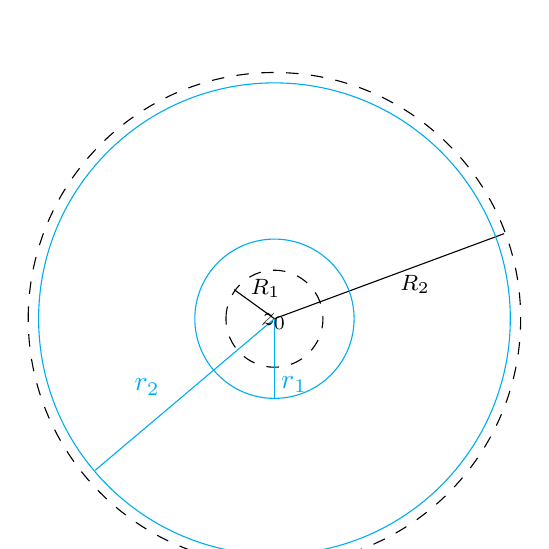
\begin{tikzpicture}[x=0.75pt,y=0.75pt,yscale=-1,xscale=1]
        %uncomment if require: \path (0,300); %set diagram left start at 0, and has height of 300
        
        %Shape: Donut [id:dp6671669505060469] 
        \draw  [dash pattern={on 4.5pt off 4.5pt}] (160.26,142.63) .. controls (160.26,129.72) and (170.72,119.26) .. (183.63,119.26) .. controls (196.54,119.26) and (207,129.72) .. (207,142.63) .. controls (207,155.54) and (196.54,166) .. (183.63,166) .. controls (170.72,166) and (160.26,155.54) .. (160.26,142.63)(65,142.63) .. controls (65,77.11) and (118.11,24) .. (183.63,24) .. controls (249.14,24) and (302.26,77.11) .. (302.26,142.63) .. controls (302.26,208.14) and (249.14,261.26) .. (183.63,261.26) .. controls (118.11,261.26) and (65,208.14) .. (65,142.63) ;
        %Straight Lines [id:da7057757873892656] 
        \draw    (164.26,128.64) -- (183.63,142.63) ;
        %Straight Lines [id:da14630762957011] 
        \draw    (183.63,142.63) -- (294.26,101.64) ;
        %Shape: Donut [id:dp20910873444708722] 
        \draw  [color=cyan  ,draw opacity=1 ] (145.26,142.63) .. controls (145.26,121.44) and (162.44,104.26) .. (183.63,104.26) .. controls (204.82,104.26) and (222,121.44) .. (222,142.63) .. controls (222,163.82) and (204.82,181) .. (183.63,181) .. controls (162.44,181) and (145.26,163.82) .. (145.26,142.63)(70,142.63) .. controls (70,79.87) and (120.87,29) .. (183.63,29) .. controls (246.38,29) and (297.26,79.87) .. (297.26,142.63) .. controls (297.26,205.38) and (246.38,256.26) .. (183.63,256.26) .. controls (120.87,256.26) and (70,205.38) .. (70,142.63) ;
        %Straight Lines [id:da5929669596751745] 
        \draw [color=cyan  ,draw opacity=1 ]   (183.63,142.63) -- (97.26,215.64) ;
        %Straight Lines [id:da5310962334011069] 
        \draw [color=cyan  ,draw opacity=1 ]   (183.63,142.63) -- (183.63,181) ;
        
        % Text Node
        \draw (175.94,139.04) node [anchor=north west][inner sep=0.75pt]    {$z_{0}$};
        % Text Node
        \draw (171,122.4) node [anchor=north west][inner sep=0.75pt]  [font=\footnotesize]  {$R_{1}$};
        % Text Node
        \draw (243,120.4) node [anchor=north west][inner sep=0.75pt]  [font=\footnotesize]  {$R_{2}$};
        % Text Node
        \draw (115,170.4) node [anchor=north west][inner sep=0.75pt]    {$\textcolor{cyan}{r_{2}}$};
        % Text Node
        \draw (185.63,169.4) node [anchor=north west][inner sep=0.75pt]    {$\textcolor{cyan}{r}\textcolor{cyan}{_{1}}$};
        
        
        \end{tikzpicture}
        \]

        Cauchy's integral formula reveals that
        $$
        f(z)=\frac{1}{2 \pi i} \int_{C_{r_2}\left(z_0\right)} \frac{f(\zeta) \d \zeta}{\zeta-z}-\frac{1}{2 \pi i} \int_{C_{r_1}\left(z_0\right)} \frac{f(\zeta) \d \zeta}{\zeta-z}
        $$
        whenever
        $$
        R_1<r_1<|z|<r_2<R_2 .
        $$
        
        These integrals are independent of $r_1$ and $r_2$ so long as $r_1<|z|<r_2$.
\end{proof}


\rmk If $n\geq 0$ and $f$ is analytic on $|z|<R_2$, then we should get that the Taylor series expansion and the Laurent expansion for the same function $f$ to match. They indeed do match by Cauchy's integral formula:\[a_{n}=\frac{f^{(n)}(z_{0})}{n!}=\frac{1}{2\pi i}\int_{C_{r}(z_{0})}\frac{f(\zeta)\d\zeta}{(\zeta-z_{0})^{n+1}}\]

\subsection{Isolated singularities}
\defn If $f$ is analytic on $0<|z-z_0|<R$ (a \underline{deleted neighbourhood} of $z_0$), then $z_0$ is an \textbf{isolated singularity} of $f$.

\defn If the principal part of the Laurent expansion for $f$ at $z_0$ is 0 (i.e. $a_{-1}=a_{-2}=\dots=0)$, then $z_0$ is a \textbf{removable singularity} of $f$. The Laurent expansion for $f$ at $z_0$ is simply a power series \(f(z)=\sum_{n=0}^{\infty}a_n(z-z_0)^n\) suggests we set $f(z_0)=a_0$, in which case $f$ is analytic at $z_0$.

\eg Observe \begin{align*}
    \frac{\sin z}{z}&= \frac{1}{z}\left(z-\frac{z^3}{3!}+\frac{z^5}{5!}-\dots\right)\\
    &= \rt{1}-\frac{z^2}{3!}+\frac{z^4}{5!}-\dots
\end{align*}
We define $f(0)=1$, so $\frac{\sin z}{z}$ is actually entire!\sidenote{This agrees with L'H\^opital's rule.}

\addlink{Conditions for removable singularity}
\begin{theorem}
    If $z_0$ is an isolated singularity of an analytic function $f$, then $z_0$ is removable \ifnif any of the following hold:\begin{enumerate}[label=(\alph*)]
        \item $f$ is bounded on some deleted neighbourhood of $z_0$
        \item $\lim_{z\to z_0}f(z)$ exists\sidenote{$\infty$ doesn't count}
        \item $\lim_{z\to z_0}(z-z_0)f(z)=0$
    \end{enumerate}
\end{theorem}
\rmk (a) and (b) implies (c), (b) implies (a).
\begin{proof}It suffices to show that (c) $\iff$ removable.
    \begin{enumerate}
        \item[($\implies$)] If $z_0$ is removable, then $f$ is analytic at $z_0$, so all of the above follow.
        
        \item[($\impliedby$)]  Suppose (c) holds. Then for all $\varepsilon>0$, there exists $0\leq r<1$ such that whenever $|z-z_0|<2r$, we have $|f(z)(z-z_0)|<\varepsilon$.
        
        Then, for all $n\geq 1$, we have \begin{align*}
            |a_{-n}|&=\left|\frac{1}{2\pi i}\int_{C_r(z_0)}f(\zeta)(\zeta-z_0)^{n-1}\d \zeta\right|\\
            &= \left|\frac{1}{2\pi i}\int_{C_r(z_0)}\rt{f(\zeta)(\zeta-z_0)}(\zeta-z_0)^{n-2}\d \zeta\right|\\
            &\leq \frac{1}{2\pi}\cdot \rt{\varepsilon}r^{n-2}2\pi r\\
            &= \varepsilon r^{n-1}\\
            &<\varepsilon
        \end{align*}
        Thus, $a_{-n}=0$ for all $n\geq 1$. The principal part of the Laurent expansion of $f$ is zero.
    \end{enumerate}
\end{proof}

\addlink{Poles}
\defn If the principal part of $f$ at $z_0$ is of the form \[\frac{a_{-n}}{(z-z_0)^{n}}+\frac{a_{-(n-1)}}{(z-z_0)^{n-1}}+\dots +\frac{a_{-1}}{(z-z_0)}\] where $a_{-n}\neq 0$, then $z_0$ is a \textbf{pole} of $f$ of order $n$.\sidenote{$n$ must be \textbf{finite} such that we can clear the denominator}

\defn A pole of order 1 is a \textbf{simple pole}.

\begin{theorem}
    If $z_0$ is an isolated singularity of $f$, then $z_0$ is a \textbf{pole} of order $\leq n$ \ifnif there is an analytic $\phi(z)$ on a \textcolor{gray}{deleted}\sidenote{Return to the full neighbourhood by the trick of removable singularity} neighbourhood of $z_0$ such that \[f(z)=\frac{\phi(z)}{(z-z_0)^n}\]
    This occurs \ifnif any of the following hold: \begin{enumerate}[label=(\alph*)]
        \item $(z-z_0)^nf(z)$ is bounded on some deleted neighbourhood of $z_0$
        \item $\lim_{z\to z_0}f(z)(z-z_0)^n$ exists
        \item $\lim_{z\to z_0}f(z)(z-z_0)^{n+1}=0$
    \end{enumerate}
\end{theorem}

\rmk We can think of poles and zeros in the following fashion: 

\begin{tabular}{ll}
   $f(z)=(z-z_0)^jF(z)$ & $g(z) = \frac{G(z)}{(z-z_0)^k}$\\
   $f$ has a zero of order $j$ at $z_0$ & $g$ has a pole of order $k$ at $z_0$\\
   $F$ doesn't vanish at $z_0$ & $G$ doesn't vanish at $z_0$
\end{tabular}
Then: \[f(z)g(z)=(z-z_0)^{\rt{j-k}}F(z)G(z)\]
\begin{itemize}
    \item If $j=k$, $z_0$ is a removable singularity for $fg$ and is not a zero.
    \item If $j>k$, then $z_0$ is a zero.
    \item If $k>j$, then $z_0$ is a pole.
\end{itemize}

Poles are nice! They could be removed like the denominators of rational functions. However, some other singularities cannot do so.

\defn If the principal part of the Laurent series for $f$ at $z_0$ is $\sum_{n=1}^{\infty}a_{-n}(z-z_0)^{-n}$ where \textbf{infinitely} many $a_{-n}\neq 0$, then $z_0$ is an essential singularity of $f$.

\rmk It is not hard to make an essential singularity: take any entire function with infinite power series. Plug in $\frac{1}{x}$ instead of $x$.

\eg $e^{\frac{1}{x}} = \sum_{n=0}^{\infty}\frac{1}{n!z^n}$ has an essential singularity at $0$.

\begin{theorem}[Casorati-Weierstrass]
    Let $z_0$ be an essential singularity of $f$. For \textbf{each} $w\in \C$\sidenote{This is wild! $f$ could almost splatter everywhere near $z_0$. There isn't a reasonable value to assign to $f(z_0)$.}, there is a sequence $z_n (n\geq 1)$ such that $z_n\to z_0$ and $f(z_n)\to w$.
\end{theorem}
\begin{proof}
    Suppose towards a contradiction that there exists $w\in \C$ such that no such $z_n$ exists. Then there exists $\varepsilon>0$ and $\delta>0$ such that when $0<|z-z_0|<\delta$, we have $|f(z)-w|\geq \varepsilon$ (that is, $f$ is not getting close to $w$). Thus, $g(z)=\frac{1}{f(z)-w}$ is analytic on $0<|z-z_0|<\delta$ and $|g(z)|\leq \frac{1}{\varepsilon}$ there. \dashuline{The singularity $z_0$ of $g$ is therefore removable.} Then $f(z)=w+\frac{1}{g(z)}$, which is either analytic or has a pole at $z_0$ (if $g(z_0)=0$). This causes a contradiction.
\end{proof}

\begin{theorem}[Great Picard]
    If $z_0$ is an essential singularity of $f$, then in any deleted neighbourhood of $z_0$, we have $f$ assuming \textbf{every} complex value \textcolor{gray}{(with at most one exception)} \textbf{infinitely} many times.
\end{theorem}

\eg $f(z)=e^{\frac{1}{z}}$ has an essential singularity at $z_0=0$. (Note $f(z)\neq 0$ is the \textcolor{gray}{exceptional value} that is never assumed.) Let $w\neq 0$ and let $z=\frac{1}{\log w}$ where $\log w$ is a nonzero logarithm of $w$\sidenote{so no 1 for $w$}. Then \[f(z)=e^{\frac{1}{1/\log w}}=e^{\log w}=w\]


\begin{theorem}[Little Picard]
    If $f$ is entire and nonconstant, then $f$ assumes every complex value, \textcolor{gray}{with at most one exception}.
\end{theorem}
\begin{proof}
    If $f$ is a nonconstant polynomial and $w\in \C$, then the polynomial $f(z)-w$ has a zero in $\C$ by the Fundamental Theorem of Algebra, so $f$ assumes the value of $w$.

    If $f$ is not a polynomial\sidenote{Non-polynomial means the Taylor series is infinite}, then $f(\frac{1}{z})$ has an essential singularity at $0$. Then use Great Picard Thm.
\end{proof}

% \section{Residue Theory}
\subsection{Residues}
\defn Let the Laurent series $f(z)=\sum_{n=-\infty}^{\infty} a_n(z-z_0)^n$ be analytic at $0<|z-z_0|<R$. The coefficient $a_{-1}$ is the \textbf{residue} of $f$ at $z_0$. Notation:\[\Res (f;z_0)=a_{-1}\]

\addlink{Residue theorem (simple version)}
\begin{theorem}[Residue, simple vers.] Let $f:\Omega\to \C$ analytic except on the isolated singularity $z_0$. Then:\[\frac{1}{2\pi i}\int_{\gamma}f(\zeta)\,d\zeta=\Res(f\cdotp z_{0}) \]
for any simple closed curve $\gamma$ in $\reg$ with $z_0$ in its interior and whose interior is contained
in $\reg$.
    \[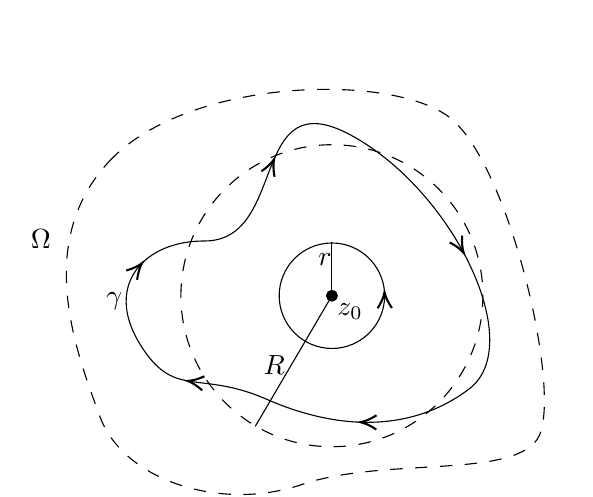
\begin{tikzpicture}[x=0.75pt,y=0.75pt,yscale=-0.7,xscale=.7]
        %uncomment if require: \path (0,300); %set diagram left start at 0, and has height of 300
        
        %Curve Lines [id:da5572659059338843] 
        \draw    (194.26,120.76) .. controls (252.26,120.76) and (224.42,9.55) .. (295.26,48) .. controls (366.09,86.45) and (416.73,192.41) .. (376.26,222.76) .. controls (335.78,253.12) and (285.26,250.76) .. (237.26,229.76) .. controls (189.26,208.76) and (173.26,230.64) .. (149.26,190.64) .. controls (125.26,150.64) and (153.26,120.51) .. (194.26,120.76) -- cycle ;
        \draw [shift={(242.18,64.55)}, rotate = 112.47] [color=black  ][line width=0.75]    (10.93,-4.9) .. controls (6.95,-2.3) and (3.31,-0.67) .. (0,0) .. controls (3.31,0.67) and (6.95,2.3) .. (10.93,4.9)   ;
        \draw [shift={(372.72,128.93)}, rotate = 240.89] [color=black  ][line width=0.75]    (10.93,-4.9) .. controls (6.95,-2.3) and (3.31,-0.67) .. (0,0) .. controls (3.31,0.67) and (6.95,2.3) .. (10.93,4.9)   ;
        \draw [shift={(301.73,245.48)}, rotate = 0.74] [color=black  ][line width=0.75]    (10.93,-4.9) .. controls (6.95,-2.3) and (3.31,-0.67) .. (0,0) .. controls (3.31,0.67) and (6.95,2.3) .. (10.93,4.9)   ;
        \draw [shift={(182.71,217.06)}, rotate = 8.82] [color=black  ][line width=0.75]    (10.93,-4.9) .. controls (6.95,-2.3) and (3.31,-0.67) .. (0,0) .. controls (3.31,0.67) and (6.95,2.3) .. (10.93,4.9)   ;
        \draw [shift={(151.34,135.99)}, rotate = 130.63] [color=black  ][line width=0.75]    (10.93,-4.9) .. controls (6.95,-2.3) and (3.31,-0.67) .. (0,0) .. controls (3.31,0.67) and (6.95,2.3) .. (10.93,4.9)   ;
        %Shape: Arc [id:dp6365443389380805] 
        \draw  [draw opacity=0] (318.31,158.43) .. controls (318.31,158.43) and (318.31,158.43) .. (318.31,158.43) .. controls (318.31,178.47) and (302.06,194.72) .. (282.02,194.72) .. controls (261.97,194.72) and (245.73,178.47) .. (245.73,158.43) .. controls (245.73,138.38) and (261.97,122.13) .. (282.02,122.13) .. controls (301.85,122.13) and (317.96,138.04) .. (318.3,157.79) -- (282.02,158.43) -- cycle ; \draw    (318.31,158.43) .. controls (318.31,158.43) and (318.31,158.43) .. (318.31,158.43) .. controls (318.31,178.47) and (302.06,194.72) .. (282.02,194.72) .. controls (261.97,194.72) and (245.73,178.47) .. (245.73,158.43) .. controls (245.73,138.38) and (261.97,122.13) .. (282.02,122.13) .. controls (301.25,122.13) and (316.99,137.1) .. (318.23,156.03) ; \draw [shift={(318.23,156.03)}, rotate = 89.02] [color=black  ][line width=0.75]    (10.93,-4.9) .. controls (6.95,-2.3) and (3.31,-0.67) .. (0,0) .. controls (3.31,0.67) and (6.95,2.3) .. (10.93,4.9)   ; 
        %Straight Lines [id:da45398740116247227] 
        \draw    (282.02,121.14) -- (282.02,158.43) ;
        \draw [shift={(282.02,158.43)}, rotate = 90] [color=black  ][fill=black  ][line width=0.75]      (0, 0) circle [x radius= 3.35, y radius= 3.35]   ;
        %Shape: Circle [id:dp805037477764748] 
        \draw  [dash pattern={on 4.5pt off 4.5pt}] (178.08,158.43) .. controls (178.08,101.02) and (224.62,54.49) .. (282.02,54.49) .. controls (339.42,54.49) and (385.95,101.02) .. (385.95,158.43) .. controls (385.95,215.83) and (339.42,262.36) .. (282.02,262.36) .. controls (224.62,262.36) and (178.08,215.83) .. (178.08,158.43) -- cycle ;
        %Straight Lines [id:da797182999934565] 
        \draw    (282.02,158.43) -- (229.26,248.39) ;
        %Shape: Polygon Curved [id:ds5262648953621514] 
        \draw  [dash pattern={on 4.5pt off 4.5pt}] (129.26,65.39) .. controls (182.26,9.39) and (318.51,4.79) .. (361.26,34.39) .. controls (404,64) and (442.26,230.39) .. (423.26,257.39) .. controls (404.26,284.39) and (317.26,269.39) .. (261.26,288.39) .. controls (205.26,307.39) and (138.26,285.39) .. (122.26,241.39) .. controls (106.26,197.39) and (76.26,121.39) .. (129.26,65.39) -- cycle ;
        
        % Text Node
        \draw (284.02,161.83) node [anchor=north west][inner sep=0.75pt]    {$z_{0}$};
        % Text Node
        \draw (270.95,127.47) node [anchor=north west][inner sep=0.75pt]    {$r$};
        % Text Node
        \draw (233.26,197.79) node [anchor=north west][inner sep=0.75pt]    {$R$};
        % Text Node
        \draw (125,154.4) node [anchor=north west][inner sep=0.75pt]    {$\gamma $};
        % Text Node
        \draw (73,111.4) node [anchor=north west][inner sep=0.75pt]    {$\Omega $};
        
        
        \end{tikzpicture}
        \]
\end{theorem}
\begin{proof}
    The Laurent expansion $f(z)\,=\,\sum_{n=-\infty}^{\infty}\,a_{n}(z\,-\,z_{0})^{n}$ converges locally uniformly on some punctured disk $0 < |z - z_0| < R$. If $r \in (0, R)$ is sufficiently small, then the deformation version of Cauchy's theorem implies \begin{align*}
        \frac{1}{2\pi i}\int_{\gamma}f(z)\d z&=\frac{1}{2\pi i}\int_{C_{r}(z_{0})}f(z)\d z\\
        &=\frac{1}{2\pi i}\int_{C_{r}(z_{0})}\sum_{n=-\infty}^{\infty}a_{n}(z-z_{0})^{n}\d z\\
        &= \sum_{n=-\infty}^{\infty}a_{n}\rt{\left(\frac{1}{2\pi i}\int_{C_{r}(z_{0})}^{}\left(z-z_{0}\right)^{n}d z\right)}
    \end{align*}
    Observe \(\rt{\left(\frac{1}{2\pi i}\int_{C_{r}(z_{0})}^{}\left(z-z_{0}\right)^{n}d z\right)}=0\) unless $n=-1$, in which it's 1. Hence:
    \begin{align*}
        \frac{1}{2\pi i}\int_{\gamma}f(z)\d z&= a_{-1}\\
        &=\Res(f;z_0)
    \end{align*}
    The interchange of sum and integral is permissible because the Laurent series converges uniformly on $C_{r}(z_0)$.
    % \tbd{finish this}
\end{proof}

\begin{lemma}\label[lemma]{residue-formula}
    If $z_0$ is a \textbf{simple} pole\sidenote{That means the pole is order 1, and the principal part of the Laurent series at that point only has 1 term.} of $f$, then \[\Res(f;z_0)=\lim_{z\to z_0}(z-z_0)f(z)\]
\end{lemma}
\begin{proof}
    Near $z_0$, we have \[f(z) = \frac{a_{-1}}{z-z_0}+a_0+a_1(z-z_0)+\dots\]
    Thus, $(z-z_0)f(z)=a_{-1}+a_0(z-z_0)+\dots$ tends to $a_{-1}$ when $z\to z_0$. So $a_{-1}=\lim_{z\to z_0}(z-z_0)f(z)$.
\end{proof}

\rmk \hyperlink{cauchys-integral-formula}{Cauchy's integral formula} is a special case of the residue formula as we rename the function to introduce a simple pole at $z_0$: \begin{align*}
    \frac{1}{2\pi i}\int_{\gamma}\frac{f(z)\d z}{z-z_0} &= \Res\left(\frac{f(z)}{z-z_0};z_0\right)\\
    &= \lim_{z\to z_0}(z-z_0)\frac{f(z)}{z-z_0}\\
    &=f(z_0)
\end{align*}

\eg Consider the improper integral
\[\int_{-\infty}^{\infty}{\frac{\cos a x}{1+x^{2}}}\d x\]
in which $a \neq 0$ is real. We assume that $a > 0$; the case $a < 0$ is similar. Since\[\left|\frac{\cos a x}{1+x^{2}}\right|\leq \frac{1}{1+x^{2}}\] on (-\infty,0] and [0,\infty), it follows that the improper integral converges by the comparison test. 

This allows us to consider the integral from $-\infty$ to $\infty$ directly, without having to consider the improper integrals over the positive and negative parts separately. Therefore, write \[\int_{-\infty}^{\infty}\frac{\cos a x}{1+x^{2}}\,d x=\mathrm{Re}\left(\operatorname*{lim}_{R\rightarrow\infty}\int_{-R}^{R}\frac{e^{i a x}}{1+x^{2}}\,d x\right)
\] where we let \[f(z)=\frac{e^{i a z}}{1+z^{2}}=\frac{e^{i a z}}{(z-i)(z+i)}\]
which has two simple poles $z=\pm i$. We focus on $i$ first.

For $R>1$ (so that $i$ is enclosed), let $\Gamma_R$ denote the semicircular curve obtained by joining $[-R, R]$ with $\gamma_R$, the upper half of the circle $|z|=R$: \[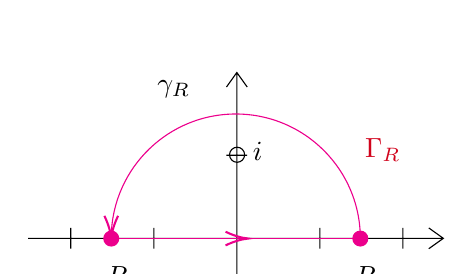
\begin{tikzpicture}[x=0.75pt,y=0.75pt,yscale=-1,xscale=1]
    %uncomment if require: \path (0,300); %set diagram left start at 0, and has height of 300
    
    %Shape: Axis 2D [id:dp3985790093437118] 
    \draw  (50,149.89) -- (250,149.89)(150.51,70) -- (150.51,170) (243,144.89) -- (250,149.89) -- (243,154.89) (145.51,77) -- (150.51,70) -- (155.51,77) (190.51,144.89) -- (190.51,154.89)(230.51,144.89) -- (230.51,154.89)(110.51,144.89) -- (110.51,154.89)(70.51,144.89) -- (70.51,154.89)(145.51,109.89) -- (155.51,109.89) ;
    \draw   ;
    %Straight Lines [id:da2085138625465428] 
    \draw [color=magenta  ,draw opacity=1 ]   (90,150) -- (210,150) ;
    \draw [shift={(210,150)}, rotate = 0] [color=magenta  ,draw opacity=1 ][fill=magenta  ,fill opacity=1 ][line width=0.75]      (0, 0) circle [x radius= 3.35, y radius= 3.35]   ;
    \draw [shift={(156,150)}, rotate = 180] [color=magenta  ,draw opacity=1 ][line width=0.75]    (10.93,-3.29) .. controls (6.95,-1.4) and (3.31,-0.3) .. (0,0) .. controls (3.31,0.3) and (6.95,1.4) .. (10.93,3.29)   ;
    \draw [shift={(90,150)}, rotate = 0] [color=magenta  ,draw opacity=1 ][fill=magenta  ,fill opacity=1 ][line width=0.75]      (0, 0) circle [x radius= 3.35, y radius= 3.35]   ;
    %Shape: Arc [id:dp46543149744952506] 
    \draw  [draw opacity=0] (89.99,150) .. controls (89.99,116.86) and (116.86,89.99) .. (150,89.99) .. controls (183.14,89.99) and (210.01,116.86) .. (210.01,150) -- (150,150) -- cycle ; \draw [color=magenta  ,draw opacity=1 ]   (90.04,147.53) .. controls (91.33,115.53) and (117.68,89.99) .. (150,89.99) .. controls (183.14,89.99) and (210.01,116.86) .. (210.01,150) ;  \draw [shift={(89.99,150)}, rotate = 270] [color=magenta  ,draw opacity=1 ][line width=0.75]    (10.93,-3.29) .. controls (6.95,-1.4) and (3.31,-0.3) .. (0,0) .. controls (3.31,0.3) and (6.95,1.4) .. (10.93,3.29)   ;
    %Shape: Circle [id:dp5979229833068613] 
    \draw   (147,109.63) .. controls (147,107.62) and (148.62,106) .. (150.63,106) .. controls (152.63,106) and (154.26,107.62) .. (154.26,109.63) .. controls (154.26,111.63) and (152.63,113.26) .. (150.63,113.26) .. controls (148.62,113.26) and (147,111.63) .. (147,109.63) -- cycle ;
    
    % Text Node
    \draw (76,162.4) node [anchor=north west][inner sep=0.75pt]    {$-R$};
    % Text Node
    \draw (206,162.4) node [anchor=north west][inner sep=0.75pt]    {$R$};
    % Text Node
    \draw (111,72.4) node [anchor=north west][inner sep=0.75pt]    {$\gamma _{R}$};
    % Text Node
    \draw (157,102.4) node [anchor=north west][inner sep=0.75pt]    {$i$};
    % Text Node
    \draw (211,100.4) node [anchor=north west][inner sep=0.75pt]    {$\textcolor[rgb]{0.82,0.01,0.11}{\Gamma _{R}}$};
    
    
    \end{tikzpicture}
    \]
Since $i$ is a pole enclosed in $\Gamma_R$, the residue theorem implies \(\int_{\Gamma_{R}}f(z)\d z=\,2\pi i\,\mathrm{Res}(f,i)\). By \cref{residue-formula}, \[\mathrm{Res}(f,i)=\operatorname*{lim}_{z\rightarrow i}(z-i)f(z)=\operatorname*{lim}_{z\rightarrow i}\frac{e^{i a z}}{(z+i)}=\frac{e^{-a}}{2i}\] so it follows that 
\[\rt{\int_{-R}^{R}{\frac{e^{i a x}}{1+x^{2}}}\d x}+\bt{\int_{\gamma_{R}}{\frac{e^{i a z}}{1+z^{2}}}\d z}=2\pi i\,\mathrm{Res}(f,i)=\pi e^{-a}\]

We look at $\bt{\int_{\gamma_{R}}{\frac{e^{i a z}}{1+z^{2}}}\d z}$. If $z=x+i y$ is on $\gamma_R$, then $y \geq 0$ and hence (since $a>0$):
\[\begin{aligned}
    \left|\bt{\int_{\gamma_{R}}{\frac{e^{i a z}}{1+z^{2}}}\d z}\right| & =\left|\int_{\gamma_R} \frac{e^{i a z}}{1+z^2} \d z\right| \\
    & \leq \pi R \sup _{z \in \gamma_R} \frac{\left|e^{i a z}\right|}{\left|1+z^2\right|} &&\text{by upper bound over length of curve}\\
    & \leq \pi R \sup _{x+i y \in \gamma_R} \frac{e^{-a y}}{R^2-1} &&\text{since }|e^{iax}|=1\\
    & =\frac{\pi R}{R^2-1}
    \end{aligned}\]
which tends to zero as $R \rightarrow \infty$.
Let $R \rightarrow \infty$ and get \[\rt{\int_{-\infty}^{\infty} \frac{e^{i a x}}{1+x^2} \d x}=\pi e^{-a}\] Thus the real part would be our answer \[\int_{-\infty}^{\infty} \frac{\cos a x}{1+x^2} d x=\pi e^{-a}\]

\section{Residue theory}
\subsection{Index, aka. winding number of a curve}
\defn Let $\gamma$ be a closed, piecewise $C^1$ curve and $z_0\notin \gamma$. The \textbf{index} (also called the \textbf{winding number}\sidenote{Number of counterclockwise loop-arounds}) of $\gamma$ with respect to $z_0$ is \[I(\gamma;z_0)=\frac{1}{2\pi i}\int_{\gamma}\frac{\d z}{z-z_0}\]

\rmk If the curve $\gamma:[a,b]\to \C$ is parameterized on $t$, and $\gamma(a)=\gamma(b)$ (closed), then let $z=\gamma(t), \d z=\gamma'(t)\d t$. Then we have \[I(\gamma;z_0)=\frac{1}{2\pi i}\int_{\gamma}\frac{\d z}{z-z_0} = \frac{1}{2\pi i}\int_{a}^{b}\frac{\gamma'(t)\d t}{\gamma(t)-z_0}\]

\begin{lemma}
    If $\gamma$ is a closed curve and $z_0\notin \gamma$, then $I(\gamma;z_0)\in \Z$.
\end{lemma}
\begin{proof}
    Parameterize $\gamma$ as above using $s$. Then \[\frac{1}{2\pi i}\int_{\gamma}\frac{\d z}{z-z_0} = \frac{1}{2\pi i}\int_{a}^{b}\frac{\gamma'(s)\d s}{\gamma(s)-z_0}\]
    Define \[g(t)=\int_{a}^{t}\frac{\gamma'(s)\d s}{\gamma(s)-z_0}\]
    Since $\gamma$ is \underline{piecewise}, by FTC, we have \[\rt{g'(t)=\frac{\gamma'(t)}{\gamma(t)-z_0}}\] for all but finitely many $t\in[a,b]$. Thus, \begin{align*}
        \frac{\d}{\d t}\left(e^{-g(t)}(\gamma(t)-z_0)\right) &= e^{-g(t)}\gamma'(t)-\rt{g'(t)}e^{-g(t)}(\gamma(t)-z_0)\\
        &= \gt{e^{-g(t)}\gamma'(t)}-\frac{\gt{\gamma'(t)}}{\bt{\gamma(t)-z_0}}\gt{e^{-g(t)}}(\bt{\gamma(t)-z_0})\\
        &= 0
    \end{align*}
    for all $t$ where $g'(t)$ exists. Therefore, $e^{-g(t)}(\gamma(t)-z_0)$ is piecewise constant. But this function is also \underline{continuous}, so it's constant! Therefore:
    \[e^{-g(b)}(\bt{\gamma(b)-z_0}) = e^{-g(a)}(\bt{\gamma(a)-z_0})\]
    The \bt{blue} terms are the same since $\gamma(a)=\gamma(b)$. Therefore, $e^{-g(b)}=e^{-g(a)}=e^0=1$ since $g(a)=0$.

    Hence, $g(b)=2\pi i n$ for some $n\in \Z$. Thus:\[I(\gamma;z_0)=\frac{1}{2\pi i}\int_{\gamma}\frac{\d z}{z-z_0} = \frac{1}{2\pi i}g(b) = n\in \Z\]
\end{proof}

\rmk Winding number essentially tracks the change of argument when the curve is traversed.
\[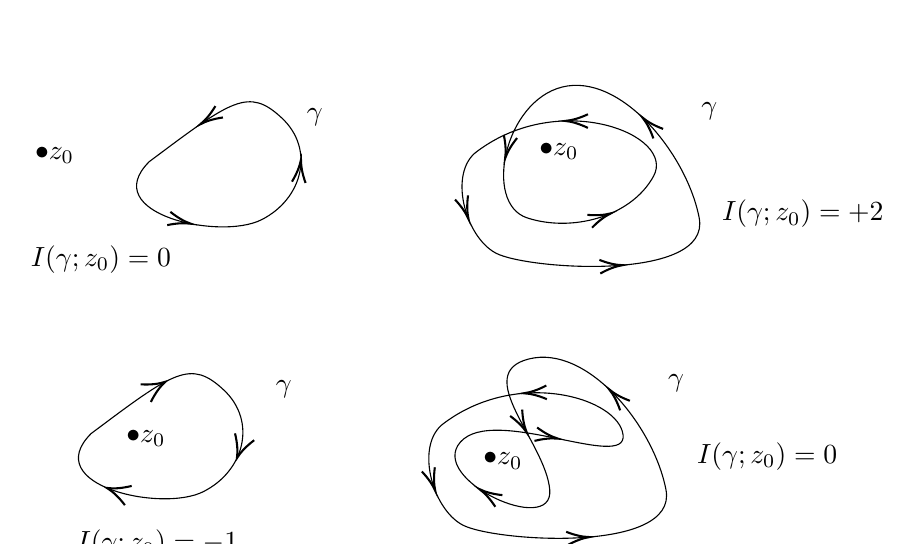
\begin{tikzpicture}[x=0.75pt,y=0.75pt,yscale=-1,xscale=1]
    %uncomment if require: \path (0,300); %set diagram left start at 0, and has height of 300
    
    %Curve Lines [id:da3037232848478386] 
    \draw    (88.26,49.14) .. controls (128.26,19.14) and (136.26,13.14) .. (152.26,28.14) .. controls (168.26,43.14) and (162.26,67.14) .. (142.26,77.14) .. controls (122.26,87.14) and (63.26,74.14) .. (88.26,49.14) -- cycle ;
    \draw [shift={(112.88,31.1)}, rotate = 326.5] [color=black  ][line width=0.75]    (10.93,-3.29) .. controls (6.95,-1.4) and (3.31,-0.3) .. (0,0) .. controls (3.31,0.3) and (6.95,1.4) .. (10.93,3.29)   ;
    \draw [shift={(161.41,48.16)}, rotate = 95.58] [color=black  ][line width=0.75]    (10.93,-3.29) .. controls (6.95,-1.4) and (3.31,-0.3) .. (0,0) .. controls (3.31,0.3) and (6.95,1.4) .. (10.93,3.29)   ;
    \draw [shift={(108.36,79)}, rotate = 193.37] [color=black  ][line width=0.75]    (10.93,-3.29) .. controls (6.95,-1.4) and (3.31,-0.3) .. (0,0) .. controls (3.31,0.3) and (6.95,1.4) .. (10.93,3.29)   ;
    %Curve Lines [id:da8924673024013423] 
    \draw    (246.26,44.14) .. controls (286.26,14.14) and (342.26,36.14) .. (331.26,56.14) .. controls (320.26,76.14) and (291.26,83.14) .. (270.26,76.14) .. controls (249.26,69.14) and (259.26,20.14) .. (287.26,13.14) .. controls (315.26,6.14) and (347.26,45.14) .. (353.26,76.14) .. controls (359.26,107.14) and (270.26,101.14) .. (255.26,93.14) .. controls (240.26,85.14) and (232.26,54.14) .. (246.26,44.14) -- cycle ;
    \draw [shift={(288.72,29.47)}, rotate = 0.38] [color=black  ][line width=0.75]    (10.93,-3.29) .. controls (6.95,-1.4) and (3.31,-0.3) .. (0,0) .. controls (3.31,0.3) and (6.95,1.4) .. (10.93,3.29)   ;
    \draw [shift={(310.76,73.98)}, rotate = 159.54] [color=black  ][line width=0.75]    (10.93,-3.29) .. controls (6.95,-1.4) and (3.31,-0.3) .. (0,0) .. controls (3.31,0.3) and (6.95,1.4) .. (10.93,3.29)   ;
    \draw [shift={(259.76,47.58)}, rotate = 283.56] [color=black  ][line width=0.75]    (10.93,-3.29) .. controls (6.95,-1.4) and (3.31,-0.3) .. (0,0) .. controls (3.31,0.3) and (6.95,1.4) .. (10.93,3.29)   ;
    \draw [shift={(325.89,27.79)}, rotate = 45.62] [color=black  ][line width=0.75]    (10.93,-3.29) .. controls (6.95,-1.4) and (3.31,-0.3) .. (0,0) .. controls (3.31,0.3) and (6.95,1.4) .. (10.93,3.29)   ;
    \draw [shift={(316.31,98.97)}, rotate = 176.13] [color=black  ][line width=0.75]    (10.93,-3.29) .. controls (6.95,-1.4) and (3.31,-0.3) .. (0,0) .. controls (3.31,0.3) and (6.95,1.4) .. (10.93,3.29)   ;
    \draw [shift={(242.13,76.76)}, rotate = 252.08] [color=black  ][line width=0.75]    (10.93,-3.29) .. controls (6.95,-1.4) and (3.31,-0.3) .. (0,0) .. controls (3.31,0.3) and (6.95,1.4) .. (10.93,3.29)   ;
    %Curve Lines [id:da4265358877348766] 
    \draw    (60.26,180.14) .. controls (100.26,150.14) and (108.26,144.14) .. (124.26,159.14) .. controls (140.26,174.14) and (134.26,198.14) .. (114.26,208.14) .. controls (94.26,218.14) and (35.26,205.14) .. (60.26,180.14) -- cycle ;
    \draw [shift={(96.08,155.14)}, rotate = 149.89] [color=black  ][line width=0.75]    (10.93,-4.9) .. controls (6.95,-2.3) and (3.31,-0.67) .. (0,0) .. controls (3.31,0.67) and (6.95,2.3) .. (10.93,4.9)   ;
    \draw [shift={(130.55,191.94)}, rotate = 289.75] [color=black  ][line width=0.75]    (10.93,-4.9) .. controls (6.95,-2.3) and (3.31,-0.67) .. (0,0) .. controls (3.31,0.67) and (6.95,2.3) .. (10.93,4.9)   ;
    \draw [shift={(67.9,206.3)}, rotate = 19.51] [color=black  ][line width=0.75]    (10.93,-4.9) .. controls (6.95,-2.3) and (3.31,-0.67) .. (0,0) .. controls (3.31,0.67) and (6.95,2.3) .. (10.93,4.9)   ;
    %Curve Lines [id:da7106931224469695] 
    \draw    (230.26,175.14) .. controls (266,148.34) and (314.51,163.05) .. (316.59,180.75) .. controls (318.67,198.45) and (254.26,166.14) .. (238.26,184.14) .. controls (222.26,202.14) and (283.26,230.14) .. (281.26,207.14) .. controls (279.26,184.14) and (243.26,151.14) .. (271.26,144.14) .. controls (299.26,137.14) and (331.26,176.14) .. (337.26,207.14) .. controls (343.26,238.14) and (254.26,232.14) .. (239.26,224.14) .. controls (224.26,216.14) and (216.26,185.14) .. (230.26,175.14) -- cycle ;
    \draw [shift={(268.81,160.68)}, rotate = 357.68] [color=black  ][line width=0.75]    (10.93,-3.29) .. controls (6.95,-1.4) and (3.31,-0.3) .. (0,0) .. controls (3.31,0.3) and (6.95,1.4) .. (10.93,3.29)   ;
    \draw [shift={(285.27,182.55)}, rotate = 191.28] [color=black  ][line width=0.75]    (10.93,-3.29) .. controls (6.95,-1.4) and (3.31,-0.3) .. (0,0) .. controls (3.31,0.3) and (6.95,1.4) .. (10.93,3.29)   ;
    \draw [shift={(247.41,206.88)}, rotate = 31.32] [color=black  ][line width=0.75]    (10.93,-3.29) .. controls (6.95,-1.4) and (3.31,-0.3) .. (0,0) .. controls (3.31,0.3) and (6.95,1.4) .. (10.93,3.29)   ;
    \draw [shift={(270.24,179.71)}, rotate = 241.88] [color=black  ][line width=0.75]    (10.93,-3.29) .. controls (6.95,-1.4) and (3.31,-0.3) .. (0,0) .. controls (3.31,0.3) and (6.95,1.4) .. (10.93,3.29)   ;
    \draw [shift={(309.89,158.79)}, rotate = 45.62] [color=black  ][line width=0.75]    (10.93,-3.29) .. controls (6.95,-1.4) and (3.31,-0.3) .. (0,0) .. controls (3.31,0.3) and (6.95,1.4) .. (10.93,3.29)   ;
    \draw [shift={(300.31,229.97)}, rotate = 176.13] [color=black  ][line width=0.75]    (10.93,-3.29) .. controls (6.95,-1.4) and (3.31,-0.3) .. (0,0) .. controls (3.31,0.3) and (6.95,1.4) .. (10.93,3.29)   ;
    \draw [shift={(226.13,207.76)}, rotate = 252.08] [color=black  ][line width=0.75]    (10.93,-3.29) .. controls (6.95,-1.4) and (3.31,-0.3) .. (0,0) .. controls (3.31,0.3) and (6.95,1.4) .. (10.93,3.29)   ;
    
    % Text Node
    \draw (32,41) node [anchor=north west][inner sep=0.75pt]   [align=left] {$\displaystyle \bullet z_{0}$};
    % Text Node
    \draw (163,22.4) node [anchor=north west][inner sep=0.75pt]    {$\gamma $};
    % Text Node
    \draw (30,88.4) node [anchor=north west][inner sep=0.75pt]    {$I( \gamma ;z_{0}) =0$};
    % Text Node
    \draw (275,39) node [anchor=north west][inner sep=0.75pt]   [align=left] {$\displaystyle \bullet z_{0}$};
    % Text Node
    \draw (353,19.4) node [anchor=north west][inner sep=0.75pt]    {$\gamma $};
    % Text Node
    \draw (363,66.4) node [anchor=north west][inner sep=0.75pt]    {$I( \gamma ;z_{0}) =+2$};
    % Text Node
    \draw (76,177) node [anchor=north west][inner sep=0.75pt]   [align=left] {$\displaystyle \bullet z_{0}$};
    % Text Node
    \draw (148,153.4) node [anchor=north west][inner sep=0.75pt]    {$\gamma $};
    % Text Node
    \draw (52,225.4) node [anchor=north west][inner sep=0.75pt]    {$I( \gamma ;z_{0}) =-1$};
    % Text Node
    \draw (248,188) node [anchor=north west][inner sep=0.75pt]   [align=left] {$\displaystyle \bullet z_{0}$};
    % Text Node
    \draw (337,150.4) node [anchor=north west][inner sep=0.75pt]    {$\gamma $};
    % Text Node
    \draw (351,183.4) node [anchor=north west][inner sep=0.75pt]    {$I( \gamma ;z_{0}) =0$};
    
    
    \end{tikzpicture}
    \]

\subsection{Simply connected domains}
\defn A region $\reg$ is \textbf{simply connected} if it has no holes. In other words: \begin{enumerate}[label=(\alph*)]
    \item $I(\gamma;z_0)=0$ for \textbf{every} closed curve $\gamma$ in $\reg$ and every $z_0\notin \reg$. 
    \item Every closed curve $\gamma$ in $\reg$ is \textbf{homotopic}\sidenote{homotopic means can be continuously deformed without passing outside $\reg$} to a point in $\reg$.
\end{enumerate}

Recall \cref{cauchys-take1}. We can now extend beyond simple curves: 
\begin{theorem}[Cauchy's, for simply connected domains]\label[theorem]{cauchys-simply-connected}
    If $\reg$ is \textbf{simply connected}, $f$ is analytic on $\reg$, then $\int_{\gamma}f(z)\d z=0$ for any closed curve $\gamma$ in $\reg$.
    \[\begin{tikzpicture}[x=0.75pt,y=0.75pt,yscale=-0.8,xscale=.8]
        %uncomment if require: \path (0,300); %set diagram left start at 0, and has height of 300
        
        %Curve Lines [id:da48836246897955626] 
        \draw    (106.26,135.14) .. controls (98.26,94.64) and (261.26,174.64) .. (276.26,167.64) .. controls (291.26,160.64) and (292.26,136.64) .. (273.26,123.64) .. controls (254.26,110.64) and (112.26,211.64) .. (106.26,135.14) -- cycle ;
        \draw [shift={(182.63,138.83)}, rotate = 18.82] [color=black  ][line width=0.75]    (10.93,-3.29) .. controls (6.95,-1.4) and (3.31,-0.3) .. (0,0) .. controls (3.31,0.3) and (6.95,1.4) .. (10.93,3.29)   ;
        \draw [shift={(287.27,152.15)}, rotate = 271.16] [color=black  ][line width=0.75]    (10.93,-3.29) .. controls (6.95,-1.4) and (3.31,-0.3) .. (0,0) .. controls (3.31,0.3) and (6.95,1.4) .. (10.93,3.29)   ;
        \draw [shift={(189.52,151.48)}, rotate = 159.72] [color=black  ][line width=0.75]    (10.93,-3.29) .. controls (6.95,-1.4) and (3.31,-0.3) .. (0,0) .. controls (3.31,0.3) and (6.95,1.4) .. (10.93,3.29)   ;
        %Shape: Polygon Curved [id:ds5031523676345244] 
        \draw  [dash pattern={on 4.5pt off 4.5pt}] (118.26,73.39) .. controls (145.26,45.39) and (227.51,58.79) .. (270.26,88.39) .. controls (313,118) and (324.26,166.39) .. (305.26,193.39) .. controls (286.26,220.39) and (227.26,207.39) .. (193.26,215.39) .. controls (159.26,223.39) and (107.26,220.39) .. (91.26,176.39) .. controls (75.26,132.39) and (91.26,101.39) .. (118.26,73.39) -- cycle ;
        
        % Text Node
        \draw (155,64.4) node [anchor=north west][inner sep=0.75pt]  [xscale=0.8,yscale=0.8]  {$\Omega $};
        
        
        \end{tikzpicture}
        \]
\end{theorem}

\addlink{Simply connected iff. antiderivative exists}
\begin{theorem}
    A region $\reg$ is \textbf{simply connected} \ifnif every analytic function $f:\reg\to\C$ has an \textbf{antiderivative} on $\reg$.
\end{theorem}
\begin{proof}We proved in \cref{convex-antiderivative} that every analytic function $f:\reg\to\C$ on a \textit{convex} $\reg$ has an antiderivative. We adapt the proof.
    \begin{itemize}[align = left]
        \item[$(\implies)$] \[\begin{tikzpicture}[x=0.75pt,y=0.75pt,yscale=-1,xscale=1]
            %uncomment if require: \path (0,300); %set diagram left start at 0, and has height of 300
            
            %Shape: Polygon Curved [id:ds5031523676345244] 
            \draw  [dash pattern={on 4.5pt off 4.5pt}] (104.26,121.89) .. controls (131.26,93.89) and (137.51,31.29) .. (180.26,60.89) .. controls (223,90.5) and (304.26,196.89) .. (285.26,223.89) .. controls (266.26,250.89) and (197.26,172.39) .. (164.26,181.89) .. controls (131.26,191.39) and (82.26,235.39) .. (66.26,191.39) .. controls (50.26,147.39) and (77.26,149.89) .. (104.26,121.89) -- cycle ;
            %Curve Lines [id:da4418491251136758] 
            \draw [color=magenta  ,draw opacity=1 ]   (104.26,159.89) .. controls (144.26,129.89) and (189.26,108.89) .. (223,138) ;
            %Curve Lines [id:da5888793969301926] 
            \draw [color=cyan  ,draw opacity=1 ]   (104.26,159.89) .. controls (125.26,176.89) and (217,165) .. (223,138) ;
            %Straight Lines [id:da9116430727041929] 
            \draw    (206,139) -- (270.52,101.89) ;
            \draw [shift={(272.26,100.89)}, rotate = 150.09] [color=black  ][line width=0.75]    (10.93,-3.29) .. controls (6.95,-1.4) and (3.31,-0.3) .. (0,0) .. controls (3.31,0.3) and (6.95,1.4) .. (10.93,3.29)   ;
            
            % Text Node
            \draw (155,64.4) node [anchor=north west][inner sep=0.75pt]  [xscale=0.8,yscale=0.8]  {$\Omega $};
            % Text Node
            \draw (223,68) node [anchor=north west][inner sep=0.75pt]  [xscale=0.8,yscale=0.8] [align=left] {No points of $\displaystyle \Omega ^{c}$ here!};
            % Text Node
            \draw (135,112.4) node [anchor=north west][inner sep=0.75pt]  [color=magenta  ,opacity=1 ,xscale=0.8,yscale=0.8]  {$\gamma _{1}$};
            % Text Node
            \draw (210,154.4) node [anchor=north west][inner sep=0.75pt]  [xscale=0.8,yscale=0.8]  {$\textcolor{cyan}{\gamma _{2}}$};
            
            
            \end{tikzpicture}
            \]
            Then use \cref{cauchys-take2-deform}.
        \item[$(\impliedby)$] Suppose BWOC that $\reg$ is \textbf{not} simply connected. Then there is a $z_0\in \reg^c$ and $\gamma$ a closed curve in $\reg$ such that $I(\gamma;z_0)\neq 0$. Then \(f(z)=\frac{1}{z-z_0}\) does not have an antiderivative on $\reg$. 
    \end{itemize}
\end{proof}

\addlink{Existence of log for non-vanishing functions}
\begin{theorem}
    If $\reg$ is simply connected and $f:\reg\to\C$ is analytic and \textbf{never 0}, then there is an analytic $g:\reg\to \C$ such that $f=e^g$. That is, it's got a log!
\end{theorem}
\begin{proof}
    The function $f'/f$ is analytic on $\reg$, thus it has an antiderivative $F$ on $\reg$. Since \[(f e^{-F})^{\prime}=f^{\prime}e^{-F}-F^{\prime}f e^{-F}=f^{\prime}e^{-F}-f^{\prime}e^{-F}=0\]it follows that $fe^{-F} =c$ for some constant $c$. Thus, $g=\log c+F$ (we may choose any fixed branch of $\log c$).
\end{proof}

\addlink{Residue theorem (general version)}
\begin{theorem}[Residue, general case]
    Let $\reg$ be a simply-connected region and let $z_1,z_2,\dots,z_n\in \reg$ be distinct. If $f:\reg\backslash\{z_{1},z_{2},\cdot\cdot\cdot,z_{n}\}\to\mathbb{C}$ is analytic and $\gamma$ is a closed curve in $\reg$ that
    passes through no $z_i$, then
    \[\frac{1}{2\pi i}\int_{\gamma}f(\zeta)\,d\zeta=\sum_{j=1}^{n}\mathrm{Res}(f;z_{j})I(\gamma,z_{j})\]
\end{theorem}

\subsection{The argument principle}
Suppose $f: \Omega \rightarrow \mathbb{C}$ is analytic and has zeros only at $z_1, z_2, \ldots, z_n \in \Omega$ (repeated according to multiplicity). Write
\[f(z)=\left(z-z_1\right)\left(z-z_2\right) \cdots\left(z-z_n\right) g(z)\]
where $g(z)$ is analytic and nonvanishing on $\Omega$. The product formula for derivatives implies
\[
\begin{aligned}
& f^{\prime}(z)=\left(z-z_2\right)\left(z-z_3\right) \cdots\left(z-z_n\right) g(z)+\left(z-z_1\right)\left(z-z_3\right) \cdots\left(z-z_n\right) g(z)+\cdots \\
&+\left(z-z_1\right)\left(z-z_2\right) \cdots\left(z-z_{n-1}\right) g(z)+\left(z-z_1\right)\left(z-z_2\right) \cdots\left(z-z_n\right) g^{\prime}(z) .
\end{aligned}
\]

Divide by $f(z)$ and obtain the \uline{logarithmic derivative of $f$}\sidenote{Since $(\log f)' = f'/f$}:
\[\rt{\frac{f^{\prime}(z)}{f(z)}}=\frac{1}{z-z_1}+\frac{1}{z-z_2}+\cdots+\frac{1}{z-z_n}+\frac{g^{\prime}(z)}{g(z)} \]

If $\gamma$ is a simple closed curve\sidenote{a simple closed curve can only envelope a finite amount of zeros!} in $\Omega$ whose interior lies in $\Omega$ and which contains each $z_i$ in its interior, then
\[\begin{aligned}
    \frac{1}{2 \pi i} \int_\gamma \rt{\frac{f^{\prime}(z)}{f(z)}} \d z & =\bt{\sum_{k=1}^n \frac{1}{2 \pi i} \int_\gamma \frac{\d z}{z-z_k}}+\gt{\frac{1}{2 \pi i} \int_\gamma \frac{g^{\prime}(z)}{g(z)} \d z} \\
    &= \sum_{k=1}^{n}I(\gamma;z_k) + \gt{0}\\
    & =\left(\sum_{k=1}^n 1\right)+0 \\
    & =n 
    \end{aligned}\]

The \gt{final integral} vanishes by Cauchy's theorem since $g^{\prime} / g$ is analytic on $\Omega$. Integrating the logarithmic derivative $\rt{f^{\prime} / f}$ of an analytic function $f$ around a closed curve $\gamma$ \uline{counts the number of zeros} of $f$, repeated according to multiplicity, inside of $\gamma$.

\theorem[The Argument Principle] Let $\Omega$ be a region in $\mathbb{C}$ and let $\gamma$ be a simple closed curve in $\Omega$ with its interior in $\Omega$. If $f:\Omega\to\mathbb{C}$ is analytic and has no zeros on $\gamma$, then the \underline{number of zeros} $Z_{f}(\gamma)$ of $f$, repeated according to multiplicity, in the interior of $\gamma$ is finite and is given by
    \[Z_{f}(\gamma)=\frac{1}{2\pi i}\int_{\gamma}\frac{f^{\prime}(z)}{f(z)}\d z\]
\begin{proof}
    In light of the preceding discussion, we only need to show that $f$ has only finitely many zeros inside of $\gamma$. Let $G$ denote the union of $\gamma$ and its interior. Since $G$ is closed and bounded, it is compact. If $f$ had infinitely many distinct zeros $z_{n}$ inside of $\gamma$, these would have an accumulation point in $G\subseteq\Omega$. The identity theorem would imply that $f$ is identically zero on $\Omega$, which contradicts the hypothesis that $f$ does not vanish on $\gamma$.
\end{proof}

\rmk Why \textit{argument} principle? Let $\gamma:[a,b]\rightarrow\mathbb{C}$ be a parametrization and consider the curve $f\circ\gamma:[a,b]\rightarrow\mathbb{C}$. The following computation shows that the number of zeros of $f$ inside $\gamma$ equals the winding number of $f\circ\gamma$ with respect to the origin:
\begin{align*}
    Z_{f}(\gamma)&=\frac{1}{2\pi i}\int_{\gamma}\frac{f^{\prime}(z)}{f(z)}\d z\\
    &=\frac{1}{2\pi i}\int_{a}^{b}\frac{f^{\prime}(\gamma(t))\gamma^{\prime}(t)\d t}{f(\gamma(t))}\\
    &=\frac{1}{2\pi i}\int_{f\circ\gamma}\frac{\d \zeta}{\zeta-0}\\
    &=I(f\circ\gamma;0)
\end{align*}

in which $\zeta=f(\gamma(t))$ and $d\zeta=f^{\prime}(\gamma(t))\gamma^{\prime}(t)\,dt$ by the chain rule.

It allows computers to compute roots with great ease. As soon as we have an error $<\frac{1}{2}$ we are done.

\[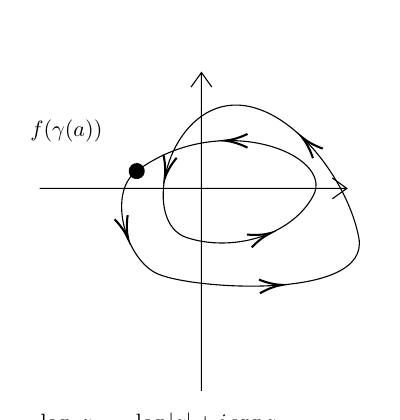
\begin{tikzpicture}[x=0.75pt,y=0.75pt,yscale=-1,xscale=1]
    %uncomment if require: \path (0,300); %set diagram left start at 0, and has height of 300
    
    %Curve Lines [id:da5005822895298122] 
    \draw    (179.26,108.14) .. controls (219.26,78.14) and (275.26,100.14) .. (264.26,120.14) .. controls (253.26,140.14) and (224.26,147.14) .. (203.26,140.14) .. controls (182.26,133.14) and (192.26,84.14) .. (220.26,77.14) .. controls (248.26,70.14) and (280.26,109.14) .. (286.26,140.14) .. controls (292.26,171.14) and (203.26,165.14) .. (188.26,157.14) .. controls (173.26,149.14) and (165.26,118.14) .. (179.26,108.14) -- cycle ;
    \draw [shift={(221.72,93.47)}, rotate = 0.38] [color=black  ][line width=0.75]    (10.93,-3.29) .. controls (6.95,-1.4) and (3.31,-0.3) .. (0,0) .. controls (3.31,0.3) and (6.95,1.4) .. (10.93,3.29)   ;
    \draw [shift={(243.76,137.98)}, rotate = 159.54] [color=black  ][line width=0.75]    (10.93,-3.29) .. controls (6.95,-1.4) and (3.31,-0.3) .. (0,0) .. controls (3.31,0.3) and (6.95,1.4) .. (10.93,3.29)   ;
    \draw [shift={(192.76,111.58)}, rotate = 283.56] [color=black  ][line width=0.75]    (10.93,-3.29) .. controls (6.95,-1.4) and (3.31,-0.3) .. (0,0) .. controls (3.31,0.3) and (6.95,1.4) .. (10.93,3.29)   ;
    \draw [shift={(258.89,91.79)}, rotate = 45.62] [color=black  ][line width=0.75]    (10.93,-3.29) .. controls (6.95,-1.4) and (3.31,-0.3) .. (0,0) .. controls (3.31,0.3) and (6.95,1.4) .. (10.93,3.29)   ;
    \draw [shift={(249.31,162.97)}, rotate = 176.13] [color=black  ][line width=0.75]    (10.93,-3.29) .. controls (6.95,-1.4) and (3.31,-0.3) .. (0,0) .. controls (3.31,0.3) and (6.95,1.4) .. (10.93,3.29)   ;
    \draw [shift={(175.13,140.76)}, rotate = 252.08] [color=black  ][line width=0.75]    (10.93,-3.29) .. controls (6.95,-1.4) and (3.31,-0.3) .. (0,0) .. controls (3.31,0.3) and (6.95,1.4) .. (10.93,3.29)   ;
    \draw [shift={(179.26,108.14)}, rotate = 323.13] [color=black  ][fill=black  ][line width=0.75]      (0, 0) circle [x radius= 3.35, y radius= 3.35]   ;
    %Shape: Axis 2D [id:dp5544761970205885] 
    \draw  (132.49,116.48) -- (280.51,116.48)(210.45,60.64) -- (210.45,214) (273.51,111.48) -- (280.51,116.48) -- (273.51,121.48) (205.45,67.64) -- (210.45,60.64) -- (215.45,67.64)  ;
    
    % Text Node
    \draw (127,82.4) node [anchor=north west][inner sep=0.75pt]  [xscale=0.8,yscale=0.8]  {$f( \gamma ( a))$};
    % Text Node
    \draw (132,223.4) node [anchor=north west][inner sep=0.75pt]  [xscale=0.8,yscale=0.8]  {$\log \ z\ =\ \log |z|+i\arg z$};
    
    
    \end{tikzpicture}
    \]  

\addlink{Root counting formula}
\begin{corollary}[Root counting formula]
    If $f:\reg\to\C$ is analytic and $\gamma$ is a simple closed curve in $\gamma$ with its interior in $\reg$ such that $f(z)\neq w$ on $\gamma$, then the number of roots of $f(z)=w$ inside $\gamma$ (with multiplicity) is $$Z_{f(z)-w}(\gamma)=\frac{1}{2\pi i}\int_{\gamma}\frac{f^{\prime}(z)}{f(z)-w}\d z$$
\end{corollary}

\eg Consider the function \[f(z)=z\left(\frac{z+\frac{1}{2}}{1+\frac{1}{2}\,z}\right)\left(\frac{z-\frac{3}{4}}{1-\frac{3}{4}\,z}\right)\left(\frac{z-\frac{4\,i}{5}}{1+\frac{4\,i}{5}\,z}\right)\] Being a product of disk automorphisms, $f$ maps $\D\to\D$. It has roots $0,\frac{-1}{2}, \frac{4i}{5}, \frac{3}{4}$. We could observe the increment of winding number corresponding to how many times zeros are included.
\drawing{0.8\linewidth}{image-8.png}

\subsection{Rouch\'e's theorem}

\begin{theorem}[Rouch\'e's] \label[theorem]{rouches-theorem}
    Let $f,g:\reg\to\C$ be analytic on $\reg$ and let $\gamma$ be a simple closed curve in $\reg$ that is homotopic to a point in $\reg$.
    If \(|f(z)-g(z)|<|f(z)|+|g(z)|\)\sidenote{observe that this is a ridiculously lenient hypothesis!} on $\gamma$,
    then $f,g$ have the same number of zeros (by multiplicity) inside $\gamma$.
\end{theorem}
\begin{proof}
    Note that the hypothesis implies that $f,g$ don't vanish on $\gamma$. Therefore, we can divide $g$ on both sides and get $\left|\frac{f}{g}-1\right|<\left|\frac{f}{g}\right|+1$ on $\gamma$. This inequality is violated whenever $f/g$ is a nonpositive real number $(\leq 0)$ on $\gamma$.

    Thus, $f/g$ maps $\gamma$ into $\C\setminus (-\infty,0]$. If $\ell(z)$ is the principal branch of the logarithm\sidenote{Recall that the principal
    branch of the logarithm has
    domain $\C\setminus (-\infty,0]$}, then $\ell\left(\frac{f}{g}\right)$ is defined on $\gamma$, and we have the logarithmic derivative $$\frac{\d}{\d z}\ell \left(\frac{f}{g}\right)=\frac{(f/g)^{\prime}}{f/g}$$
    on some open set containing $\gamma$. The Fundamental Theorem of Calculus and the argument
    principle imply 
    \begin{align*}
        0&\stackrel{FTC}{=}\frac{1}{2\pi i}\int_{\gamma}\frac{(f(z)/g(z))^{\prime}}{f(z)/g(z)}\d z\\ 
        &=\frac{1}{2\pi i}\int_{\gamma}\left(\frac{f^{\prime}(z)g(z)-f(z)g^{\prime}(z)}{g(z)^{2}}\cdot\frac{g(z)}{f(z)}\right)\d z\\ 
        &=\frac{1}{2\pi i}\int_{\gamma}\left(\frac{f^{\prime}(z)}{f(z)}-\frac{g^{\prime}(z)}{g(z)}\right)\d z\\ 
        &=\rt{\frac{1}{2\pi i}\int_{\gamma}\frac{f^{\prime}(z)}{f(z)}\d z}-\bt{\frac{1}{2\pi i}\int_{\gamma}\frac{g^{\prime}(z)}{g(z)}\d z}\\ 
        &=\rt{Z_{f}(\gamma)}-\bt{Z_{g}(\gamma)}
    \end{align*}
\end{proof}

\addlink{Weak Rouch\'e's theorem}
\begin{corollary}[Weak Rouch\'e's]\label[corollary]{weak-rouches}
    Let $f,h:\Omega\to\mathbb{C}$ be analytic on $\Omega$ and $\gamma$ be a closed curve in $\Omega$ that is homotopic to a point in $\Omega$. If $|h(z)|<|f(z)|$\sidenote{think $h$ perturbs $f$ a little bit} for all $z\in\gamma$, then $f$ and $f+h$ have the same number of zeros (counted by multiplicity) inside of $\gamma$.
\end{corollary}
\begin{proof}
    If $z\in \gamma$, then $$\left|\left(f(z)+h(z)\right)-f(z)\right|=|h(z)|<\rt{|f(z)|\leq|f(z)+h(z)|+|f(z)|}.$$
    \rt{This} is a significant overestimation. Let $f+h$ be the $g$ in \cref{rouches-theorem} and obtain the result.
\end{proof}

\rmk How to think about \cref{weak-rouches}? Let $f(z)$ where $z\in \gamma$ be the position of a dog walker in a garden. Let 0 be a tree. Let $f(z)+h(z)$ denote the position of the dog on leash. The fact that $|h|<|f|$ means the leash is shorter than the distance from the walker to the origin. We observe that the dog cannot walk around the tree more times than the owner!

\subsubsection{Fundamental Theorem of Algebra}
\begin{corollary}[FTA]
    If $p$ is a polynomial of degree $n \geq 1$, then $p(z)$ has exactly $n$ roots in $\C$, counted according to multiplicity.
\end{corollary}
\begin{proof}
    If $p(z)=a_{n}z^{n}+a_{n-1}z^{n-1}+\cdots+a_{0}$ and $a_{n}\neq0$, then\sidenote{a polynomial is dominated by its leading term} \[\lim_{z\to\infty}\frac{p(z)}{a_{n}z^{n}}=1\]
    For sufficiently large $R>0$,
    $$|z|=R\quad\implies\quad\left|\frac{p(z)}{a_{n}z^{n}}-1\right|<1$$
    and hence   
    $$|z|=R\quad\implies\quad\left|\frac{p(z)}{f(z)}-\frac{a_{n}z^{n}}{g(z)}\right|<\left|\frac{a_{n}z^{n}}{g(z)}\right|.$$
    Weak Rouche's theorem (\cref{weak-rouches}) implies that $p(z)$ and $a_nz^{n}$ have the same number of zeros (namely $n$), counted according to multiplicities, inside any disk of sufficiently large radius.    
\end{proof}

\eg Consider the transcendental equation $e^{z}=3z^{n}$\sidenote{observe this is hard to solve by non-numerical methods}, in which $n$ is a positive integer. How many solutions does it have inside the unit circle?

Let $$f(z)=e^{z}-3z^{n}\qquad\text{and}\qquad g(z)=-3z^{n}$$ and note that $g$ has precisely $n$ zeros (counted by multiplicity) in $|z|<1$. 

For $|z|=1$,
$$|\underbrace{(e^{z}-3z^{n})}_{f(z)}-\underbrace{(-3z^{n})}_{g(z)}|=|e^{z}|=e^{\operatorname{Re}z}\leq e<3=|\underbrace{-3z^{n}}_{g(z)}|\leq \underbrace{-3z^{n}}_{g(z)}| + \underbrace{e^{z}-3z^n}_{f(z)}|$$
Rouch\'e's theorem (\cref{rouches-theorem}) implies that $f$ has exactly $n$ roots inside the unit circle.

\rmk We can also use the argument principle to get $Z_f(\gamma)=I(f\circ \gamma; 0)$ and integrate numerically up to a precision of $1/2$, but Rouch\'e's theorem is certainly more computationally light.

\eg Consider

$$f(z)=z^{9}-8z^{2}+5.$$

Since $\deg f=9$ we do not expect to find its zeros in closed form.\sidenote{cf. Galois theory} 
However, we can use Rouch\'e's theorem to help locate their general whereabouts.

Since $f$ has real coefficients and odd degree, the \textbf{intermediate value theorem} implies that $f$ has at least one real root. Since $f$ has real coefficients, the non-real roots of $f$ must appear in complex conjugate pairs. Thus, $f$ has an odd number of real roots.

For $|z|=\frac{3}{2}$, \begin{align*}
    |\underbrace{z^{9}-8z^{2}+5}_{f}-\underbrace{z^{9}}_{g}|&=|8z^{2}-5|\\
    &\leq8(\tfrac{3}{2})^{2}+5\\
    &=23\\
    &<(\tfrac{3}{2})^{9}\quad(\approx38.44)\\
    &=\underbrace{|z^9|}_{g}
\end{align*}
Rouch\'e's theorem implies $f$ has 9 zeros (counted according to multiplicity) in $|z|<\frac{3}{2}$. By FTA, these are all roots of $f$.

Now we look at smaller regions to gauge the distribution of the roots of $f$.

For $|z|=1$,\sidenote{this $g$ has 2 roots} \begin{align*}
    |\underbrace{z^{9}-8z^{2}+5}_{f}\ -\ \underbrace{(-8z^{2}+5)}_{g}|&=|z^{9}|\\
    &=1<3\leq |\underbrace{-8z^{2}+5}_{g}|
\end{align*}
Rouch\'e's theorem implies $f$ has 2 zeros, counted by multiplicity, in $|z|<1$.

For $|z|=\frac{1}{2}$,\sidenote{this $g$ has 0 roots}\begin{align*}
    |\underbrace{z^{9}-8z^{2}+5}_{f}\ +\underbrace{-5}_{g}|&=|z^{9}-8z^{2}|\\
    &\leq|z|^{9}+8|z|^{2}\\
    &=\frac{1}{2^{9}}+2\\
    &<5=|\underbrace{-5}_{g}|
\end{align*}
Rouch\'e's theorem implies $f$ has no zeros in $|z|<\frac{1}{2}$.

\subsection{Local mapping theorem}
\begin{theorem}[Local mapping]
    Suppose that $f:\Omega\to\mathbb{C}$ is analytic and nonconstant. Let $z_{0}\in\Omega$ and let the value $w_{0}=f(z_{0})$ be assumed with multiplicity $n$\sidenote{$f(z)-w_{0}$ has a zero of order $n$ at $z_{0}$}. 
    
    For each sufficiently small $\delta>0$, there exists $\varepsilon>0$ such that $0<|w_{0}-w_{0}|<\varepsilon$ implies that $f$ assumes the value $w$ at exactly $n$ distinct points in $0<|z-z_{0}|<\delta$, each with multiplicity one.
    \[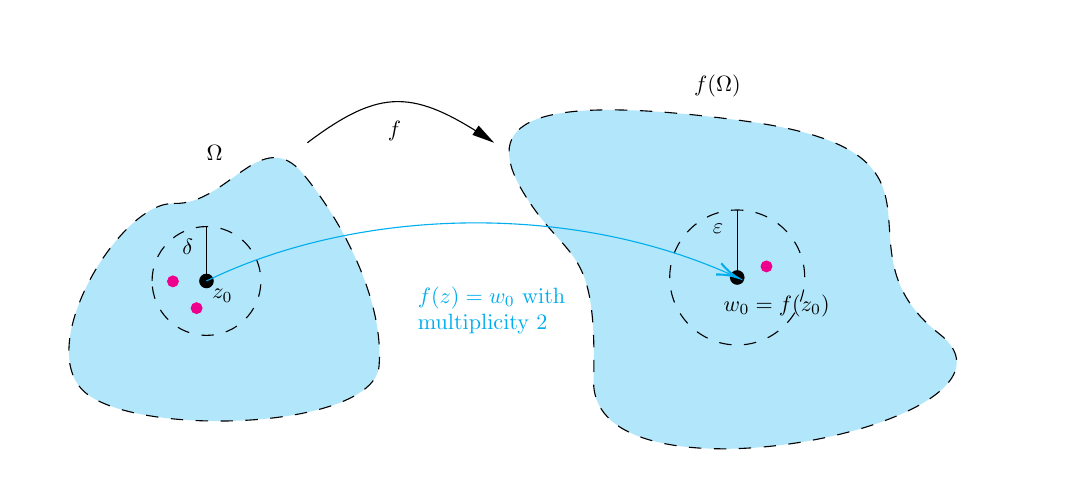
\begin{tikzpicture}[x=0.75pt,y=0.75pt,yscale=-.9,xscale=.9]
        %uncomment if require: \path (0,300); %set diagram left start at 0, and has height of 300
        
        %Shape: Polygon Curved [id:ds199380446597198] 
        \draw  [fill=cyan  ,fill opacity=0.3 ][dash pattern={on 4.5pt off 4.5pt}] (112.5,123.5) .. controls (141.5,124.5) and (159.5,80.5) .. (182,108) .. controls (204.5,135.5) and (224.91,176.75) .. (222.42,210.25) .. controls (219.92,243.75) and (99.59,248.75) .. (67.08,226.25) .. controls (34.58,203.75) and (83.5,122.5) .. (112.5,123.5) -- cycle ;
        %Shape: Polygon Curved [id:ds46424882675538726] 
        \draw  [fill=cyan  ,fill opacity=0.3 ][dash pattern={on 4.5pt off 4.5pt}] (301.25,120.25) .. controls (278.25,84.25) and (291.25,62.25) .. (417.25,79.25) .. controls (543.25,96.25) and (462.25,146.25) .. (522.25,193.25) .. controls (582.25,240.25) and (335.25,291.25) .. (337.25,218.25) .. controls (339.25,145.25) and (324.25,156.25) .. (301.25,120.25) -- cycle ;
        %Curve Lines [id:da3742131578130379] 
        \draw    (184,91) .. controls (223.6,61.3) and (240.91,62.23) .. (282.73,90.15) ;
        \draw [shift={(284,91)}, rotate = 213.92] [fill=black  ][line width=0.08]  [draw opacity=0] (12,-3) -- (0,0) -- (12,3) -- cycle    ;
        %Shape: Circle [id:dp6048852286733579] 
        \draw  [dash pattern={on 4.5pt off 4.5pt}] (100.87,165) .. controls (100.87,148.91) and (113.91,135.87) .. (130,135.87) .. controls (146.09,135.87) and (159.13,148.91) .. (159.13,165) .. controls (159.13,181.09) and (146.09,194.13) .. (130,194.13) .. controls (113.91,194.13) and (100.87,181.09) .. (100.87,165) -- cycle ;
        %Shape: Circle [id:dp9734988957299731] 
        \draw  [dash pattern={on 4.5pt off 4.5pt}] (378,163.13) .. controls (378,143.18) and (394.18,127) .. (414.13,127) .. controls (434.08,127) and (450.26,143.18) .. (450.26,163.13) .. controls (450.26,183.08) and (434.08,199.26) .. (414.13,199.26) .. controls (394.18,199.26) and (378,183.08) .. (378,163.13) -- cycle ;
        %Straight Lines [id:da4544217864520035] 
        \draw    (130,135.87) -- (130,165) ;
        \draw [shift={(130,165)}, rotate = 90] [color=black  ][fill=black  ][line width=0.75]      (0, 0) circle [x radius= 3.35, y radius= 3.35]   ;
        %Straight Lines [id:da37495890514322716] 
        \draw    (414.13,127) -- (414.13,163.13) ;
        \draw [shift={(414.13,163.13)}, rotate = 90] [color=black  ][fill=black  ][line width=0.75]      (0, 0) circle [x radius= 3.35, y radius= 3.35]   ;
        %Curve Lines [id:da6838529182425372] 
        \draw [color=cyan  ,draw opacity=1 ]   (130,165) .. controls (209.85,126.09) and (324.11,121.93) .. (412.79,162.51) ;
        \draw [shift={(414.13,163.13)}, rotate = 204.89] [color=cyan  ,draw opacity=1 ][line width=0.75]    (10.93,-3.29) .. controls (6.95,-1.4) and (3.31,-0.3) .. (0,0) .. controls (3.31,0.3) and (6.95,1.4) .. (10.93,3.29)   ;
        %Shape: Circle [id:dp11568574422525191] 
        \draw  [color=magenta  ,draw opacity=1 ][fill=magenta  ,fill opacity=1 ] (432.67,157.21) .. controls (432.67,155.62) and (431.38,154.33) .. (429.79,154.33) .. controls (428.21,154.33) and (426.92,155.62) .. (426.92,157.21) .. controls (426.92,158.79) and (428.21,160.08) .. (429.79,160.08) .. controls (431.38,160.08) and (432.67,158.79) .. (432.67,157.21) -- cycle ;
        %Shape: Circle [id:dp848292388840219] 
        \draw  [color=magenta  ,draw opacity=1 ][fill=magenta  ,fill opacity=1 ] (127.59,179.54) .. controls (127.59,177.95) and (126.3,176.67) .. (124.71,176.67) .. controls (123.13,176.67) and (121.84,177.95) .. (121.84,179.54) .. controls (121.84,181.12) and (123.13,182.41) .. (124.71,182.41) .. controls (126.3,182.41) and (127.59,181.12) .. (127.59,179.54) -- cycle ;
        %Shape: Circle [id:dp1795278145704764] 
        \draw  [color=magenta  ,draw opacity=1 ][fill=magenta  ,fill opacity=1 ] (114.92,165.21) .. controls (114.92,163.62) and (113.63,162.33) .. (112.05,162.33) .. controls (110.46,162.33) and (109.18,163.62) .. (109.18,165.21) .. controls (109.18,166.79) and (110.46,168.08) .. (112.05,168.08) .. controls (113.63,168.08) and (114.92,166.79) .. (114.92,165.21) -- cycle ;
        
        % Text Node
        \draw (129,91.4) node [anchor=north west][inner sep=0.75pt]  [xscale=0.8,yscale=0.8]  {$\Omega $};
        % Text Node
        \draw (132,168.4) node [anchor=north west][inner sep=0.75pt]  [xscale=0.8,yscale=0.8]  {$z_{0}$};
        % Text Node
        \draw (405.75,171.09) node [anchor=north west][inner sep=0.75pt]  [xscale=0.8,yscale=0.8]  {$w_{0} =f( z_{0})$};
        % Text Node
        \draw (226,78.4) node [anchor=north west][inner sep=0.75pt]  [xscale=0.8,yscale=0.8]  {$f$};
        % Text Node
        \draw (390,53.4) node [anchor=north west][inner sep=0.75pt]  [xscale=0.8,yscale=0.8]  {$f( \Omega )$};
        % Text Node
        \draw (115.95,141.47) node [anchor=north west][inner sep=0.75pt]  [xscale=0.8,yscale=0.8]  {$\delta $};
        % Text Node
        \draw (399.95,133.47) node [anchor=north west][inner sep=0.75pt]  [xscale=0.8,yscale=0.8]  {$\varepsilon $};
        % Text Node
        \draw (242,167) node [anchor=north west][inner sep=0.75pt]  [color=cyan  ,opacity=1 ,xscale=0.8,yscale=0.8] [align=left] {$\displaystyle f( z) =w_{0}$ with \\multiplicity 2};
        
        
        \end{tikzpicture}
        \]
\end{theorem}
\begin{proof}
    Since the zeros of nonconstant analytic functions are isolated, there is an $r>0$ such that $B_{r}(z_{0})^{-}$ is contained in $\Omega$ and
$$0<|z-z_{0}|\leq r\quad\implies\quad f(z)\neq w_{0}\quad\text{and}\quad f^{\prime}(z)\neq0$$
For $0<\delta<r$,\sidenote{strictly $>0$ because $f(z)\neq w_0$ and circle $|z-z_0|=\delta$ is compact}
$$\varepsilon=\min_{|z-z_{0}|=\delta}|f(z)-w_{0}|>0$$
since the circle $|z-z_{0}|=\delta$ is compact and $f(z)\neq w_{0}$ on $|z-z_{0}|\leq r$.

If $0<|w-w_{0}|<\varepsilon$ and $|z-z_{0}|=\delta$, then
$$|\underbrace{(f(z)-w_{0})}_{F(z)}\ -\ \underbrace{(f(z)-w)}_{G(z)}|=|w-w_{0}|<\varepsilon\leq|\underbrace{f(z)-w_{0}}_{F(z)}|$$
Rouche's theorem implies that $f-w_{0}$ and $f-w$ have the same number of zeros in $B_{\delta}(z_{0})$. 

By isolated zeros, we know that $f-w_{0}$ has a zero of order $n$ at $z_{0}$ and no other zeros in $B_{\delta}(z_{0})$. Therefore, $f-w$ has exactly $n$ zeros, counted according to multiplicity, in $B_{\delta}(z_{0})$. These zeros must be simple since $f^{\prime}$ does not vanish on $B_{\delta}(z_{0})$ by isolated zeros. Thus, $f$ assumes the value $w_0$ at exactly $n$ distinct points in $B_{\delta}(z_{0})$.
\end{proof}

\addlink{Open mapping property}
\begin{corollary}[Open mapping property]
    If $f:\Omega\to\mathbb{C}$ is analytic and nonconstant, then if $U\subseteq\Omega$ is open, then $f(U)$ is open.\sidenote{i.e. blobs go to blobs}
\end{corollary}
\begin{proof}
    It suffices to show that $f(\Omega)$ is open since if $U\subseteq\Omega$ is open, we may consider the restriction $f:U\to\mathbb{C}$ instead. 
    
    Let $z_{0}\in\Omega$, and $w_{0}=f(z_{0})$. If $\delta>0$ is sufficiently small, then $B_{\delta}(z_{0})\subseteq\Omega$ and $f(\Omega)$ contains $B_{\varepsilon}(w_{0})$ for some $\varepsilon>0$. Thus, $f(\Omega)$ is open.
\end{proof}

\addlink{Maximum modulus principle}
\begin{theorem}
    If $f:\Omega\to\mathbb{C}$ is analytic and $|f|$ has a local maximum in $\Omega$, then $f$ is constant.\sidenote{i.e. local maximum cannot be inside the region and not on the boundary.}
\end{theorem}
\begin{proof}
    Suppose that $f:\Omega\to\mathbb{C}$ is analytic and nonconstant. If $z_{0}\in U\subseteq\Omega$, in which $U$ is open, then $f(U)$ is open and contains $f(z_{0})$. Since $f(\Omega)$ contains points of modulus larger than $f(z_{0})$, it follows that $|f(z)|$ does not have a local maximum at $z_{0}$.
\end{proof}

\subsection{Injectivity}
\begin{corollary}[Local injectivity]\label[corollary]{local-injective}
    If $f$ is analytic near $z_{0}$ and $f^{\prime}(z_{0})\neq0$, then $f$ is \textbf{injective} on some neighborhood of $z_{0}$.
\end{corollary}
\begin{proof}[Proof ($n=1$ case of LMT)]
    Let $w_{0}=f(z_{0})$. If $f^{\prime}(z_{0})\neq0$, then $f(z)-w_{0}$ has a zero of order one at $z_{0}$. 
    
    By the local mapping theorem, for each sufficiently small $\delta>0$ there exists $\varepsilon>0$ such that if $0<|w-w_{0}|<\varepsilon$, then $f$ assumes the value $w$ at \underline{exactly one point} in $0<|z-z_{0}|<\delta$.
\end{proof}

\eg One cannot conclude anything about global injectivity using the preceding
results. For example, $f(z)=e^z$ satisfies $f'(z)\neq 0$ for all $z$, but it is NOT injective on $\C$ since it is $2\pi i$-periodic. It is, however, injective on a small neighborhood of any given point.
\[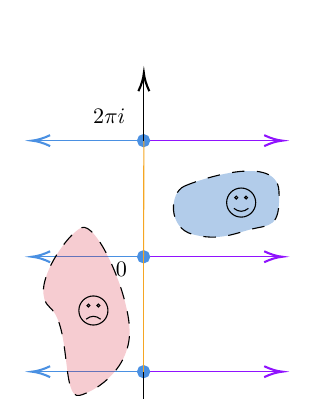
\begin{tikzpicture}[x=0.75pt,y=0.75pt,yscale=-.8,xscale=.8]
    %uncomment if require: \path (0,300); %set diagram left start at 0, and has height of 300
    
    %Straight Lines [id:da22311048865083394] 
    \draw [color={rgb, 255:red, 144; green, 19; blue, 254 }  ,draw opacity=1 ]   (139.98,150.39) -- (221.55,150.39) ;
    \draw [shift={(223.55,150.39)}, rotate = 180] [color={rgb, 255:red, 144; green, 19; blue, 254 }  ,draw opacity=1 ][line width=0.75]    (10.93,-3.29) .. controls (6.95,-1.4) and (3.31,-0.3) .. (0,0) .. controls (3.31,0.3) and (6.95,1.4) .. (10.93,3.29)   ;
    %Straight Lines [id:da18708491874048527] 
    \draw [color={rgb, 255:red, 74; green, 144; blue, 226 }  ,draw opacity=1 ]   (139.98,150.39) -- (74.75,150.39) ;
    \draw [shift={(72.75,150.39)}, rotate = 360] [color={rgb, 255:red, 74; green, 144; blue, 226 }  ,draw opacity=1 ][line width=0.75]    (10.93,-3.29) .. controls (6.95,-1.4) and (3.31,-0.3) .. (0,0) .. controls (3.31,0.3) and (6.95,1.4) .. (10.93,3.29)   ;
    \draw [shift={(139.98,150.39)}, rotate = 180] [color={rgb, 255:red, 74; green, 144; blue, 226 }  ,draw opacity=1 ][fill={rgb, 255:red, 74; green, 144; blue, 226 }  ,fill opacity=1 ][line width=0.75]      (0, 0) circle [x radius= 3.35, y radius= 3.35]   ;
    %Straight Lines [id:da5220594818080124] 
    \draw [color={rgb, 255:red, 144; green, 19; blue, 254 }  ,draw opacity=1 ]   (139.98,219.6) -- (221.55,219.6) ;
    \draw [shift={(223.55,219.6)}, rotate = 180] [color={rgb, 255:red, 144; green, 19; blue, 254 }  ,draw opacity=1 ][line width=0.75]    (10.93,-3.29) .. controls (6.95,-1.4) and (3.31,-0.3) .. (0,0) .. controls (3.31,0.3) and (6.95,1.4) .. (10.93,3.29)   ;
    %Straight Lines [id:da9258702521147173] 
    \draw [color={rgb, 255:red, 74; green, 144; blue, 226 }  ,draw opacity=1 ]   (139.98,219.6) -- (74.75,219.6) ;
    \draw [shift={(72.75,219.6)}, rotate = 360] [color={rgb, 255:red, 74; green, 144; blue, 226 }  ,draw opacity=1 ][line width=0.75]    (10.93,-3.29) .. controls (6.95,-1.4) and (3.31,-0.3) .. (0,0) .. controls (3.31,0.3) and (6.95,1.4) .. (10.93,3.29)   ;
    \draw [shift={(139.98,219.6)}, rotate = 180] [color={rgb, 255:red, 74; green, 144; blue, 226 }  ,draw opacity=1 ][fill={rgb, 255:red, 74; green, 144; blue, 226 }  ,fill opacity=1 ][line width=0.75]      (0, 0) circle [x radius= 3.35, y radius= 3.35]   ;
    %Straight Lines [id:da5593976322909007] 
    \draw [color={rgb, 255:red, 144; green, 19; blue, 254 }  ,draw opacity=1 ]   (140.15,80.46) -- (221.55,80.46) ;
    \draw [shift={(223.55,80.46)}, rotate = 180] [color={rgb, 255:red, 144; green, 19; blue, 254 }  ,draw opacity=1 ][line width=0.75]    (10.93,-3.29) .. controls (6.95,-1.4) and (3.31,-0.3) .. (0,0) .. controls (3.31,0.3) and (6.95,1.4) .. (10.93,3.29)   ;
    %Straight Lines [id:da4484234283967916] 
    \draw [color={rgb, 255:red, 74; green, 144; blue, 226 }  ,draw opacity=1 ]   (139.98,80.46) -- (74.75,80.46) ;
    \draw [shift={(72.75,80.46)}, rotate = 360] [color={rgb, 255:red, 74; green, 144; blue, 226 }  ,draw opacity=1 ][line width=0.75]    (10.93,-3.29) .. controls (6.95,-1.4) and (3.31,-0.3) .. (0,0) .. controls (3.31,0.3) and (6.95,1.4) .. (10.93,3.29)   ;
    \draw [shift={(139.98,80.46)}, rotate = 180] [color={rgb, 255:red, 74; green, 144; blue, 226 }  ,draw opacity=1 ][fill={rgb, 255:red, 74; green, 144; blue, 226 }  ,fill opacity=1 ][line width=0.75]      (0, 0) circle [x radius= 3.35, y radius= 3.35]   ;
    %Straight Lines [id:da7352916869080699] 
    \draw [color={rgb, 255:red, 245; green, 166; blue, 35 }  ,draw opacity=1 ]   (139.98,150.39) -- (140.15,80.46) ;
    %Straight Lines [id:da6707886332001725] 
    \draw [color={rgb, 255:red, 245; green, 166; blue, 35 }  ,draw opacity=1 ]   (139.98,219.6) -- (139.98,150.39) ;
    %Straight Lines [id:da641633314187205] 
    \draw    (140.15,80.46) -- (140.15,41.72) ;
    \draw [shift={(140.15,39.72)}, rotate = 90] [color={rgb, 255:red, 0; green, 0; blue, 0 }  ][line width=0.75]    (10.93,-3.29) .. controls (6.95,-1.4) and (3.31,-0.3) .. (0,0) .. controls (3.31,0.3) and (6.95,1.4) .. (10.93,3.29)   ;
    %Straight Lines [id:da5156062182444048] 
    \draw    (139.98,245.34) -- (139.98,219.6) ;
    %Shape: Polygon Curved [id:ds45793839415006077] 
    \draw  [fill={rgb, 255:red, 0; green, 87; blue, 184 }  ,fill opacity=0.3 ][dash pattern={on 4.5pt off 4.5pt}] (164.51,107.89) .. controls (173.51,103.89) and (220.51,87.89) .. (221.51,110.89) .. controls (222.51,133.89) and (215.51,130.89) .. (204.51,133.89) .. controls (193.51,136.89) and (184.51,140.89) .. (169.51,136.89) .. controls (154.51,132.89) and (155.51,111.89) .. (164.51,107.89) -- cycle ;
    %Shape: Smiley Face [id:dp6908153421809746] 
    \draw   (190,117.75) .. controls (190,112.92) and (193.92,109) .. (198.75,109) .. controls (203.59,109) and (207.51,112.92) .. (207.51,117.75) .. controls (207.51,122.59) and (203.59,126.51) .. (198.75,126.51) .. controls (193.92,126.51) and (190,122.59) .. (190,117.75) -- cycle ; \draw   (194.9,114.78) .. controls (194.9,114.29) and (195.29,113.9) .. (195.78,113.9) .. controls (196.26,113.9) and (196.65,114.29) .. (196.65,114.78) .. controls (196.65,115.26) and (196.26,115.65) .. (195.78,115.65) .. controls (195.29,115.65) and (194.9,115.26) .. (194.9,114.78) -- cycle ; \draw   (200.85,114.78) .. controls (200.85,114.29) and (201.25,113.9) .. (201.73,113.9) .. controls (202.21,113.9) and (202.6,114.29) .. (202.6,114.78) .. controls (202.6,115.26) and (202.21,115.65) .. (201.73,115.65) .. controls (201.25,115.65) and (200.85,115.26) .. (200.85,114.78) -- cycle ; \draw   (194.38,121.25) .. controls (197.29,123.59) and (200.21,123.59) .. (203.13,121.25) ;
    %Shape: Polygon Curved [id:ds49041244870492706] 
    \draw  [fill={rgb, 255:red, 208; green, 2; blue, 27 }  ,fill opacity=0.2 ][dash pattern={on 4.5pt off 4.5pt}] (102.51,132.89) .. controls (111.51,128.89) and (130.51,170.89) .. (131.51,193.89) .. controls (132.51,216.89) and (112.51,230.89) .. (101.51,233.89) .. controls (90.51,236.89) and (96.51,191.89) .. (83.51,180.89) .. controls (70.51,169.89) and (93.51,136.89) .. (102.51,132.89) -- cycle ;
    %Shape: Smiley Face [id:dp8093188113184564] 
    \draw   (101,182.75) .. controls (101,177.92) and (104.92,174) .. (109.75,174) .. controls (114.59,174) and (118.51,177.92) .. (118.51,182.75) .. controls (118.51,187.59) and (114.59,191.51) .. (109.75,191.51) .. controls (104.92,191.51) and (101,187.59) .. (101,182.75) -- cycle ; \draw   (105.9,179.78) .. controls (105.9,179.29) and (106.29,178.9) .. (106.78,178.9) .. controls (107.26,178.9) and (107.65,179.29) .. (107.65,179.78) .. controls (107.65,180.26) and (107.26,180.65) .. (106.78,180.65) .. controls (106.29,180.65) and (105.9,180.26) .. (105.9,179.78) -- cycle ; \draw   (111.85,179.78) .. controls (111.85,179.29) and (112.25,178.9) .. (112.73,178.9) .. controls (113.21,178.9) and (113.6,179.29) .. (113.6,179.78) .. controls (113.6,180.26) and (113.21,180.65) .. (112.73,180.65) .. controls (112.25,180.65) and (111.85,180.26) .. (111.85,179.78) -- cycle ; \draw   (105.38,188) .. controls (108.29,185.67) and (111.21,185.67) .. (114.13,188) ;
    
    % Text Node
    \draw (122,152.4) node [anchor=north west][inner sep=0.75pt]  [xscale=0.8,yscale=0.8]  {$0$};
    % Text Node
    \draw (108.4,60) node [anchor=north west][inner sep=0.75pt]  [xscale=0.8,yscale=0.8]  {$2\pi i$};
    
    
    \end{tikzpicture}
    \]

\noneg \cref{local-injective} does not hold for functions of a real variable (if one interprets
“analytic” as “differentiable”). Using the definition of the derivative, one can show that
$$f(x)=\begin{cases}x+2x^{2}\sin\frac{1}{x}&x\neq0,\\ 0&x=0,\end{cases}$$
satisfies $f^{\prime}(0)=1>0$. One might assume that $f$ is injective in some small neighborhood of $0$. This turns out to be false (see Figure 1). Indeed, the derivative of $f$ is
$$f^{\prime}(x)=\begin{cases}1+4x\sin\frac{1}{x}-2\cos\frac{1}{x}&x\neq0,\\ 1&x=0,\end{cases}$$
which oscillates between arbitrarily large positive and negative values \textit{infinitely often} as $x$ approaches $0$. \sidenote{In complex land, $\sin(1/x)$ has an essential singularity at 0}
Thus, $f$ is neither increasing (nor decreasing) on any open interval containing $0$. In particular, $f$ is not injective on any neighborhood of $0$.
\[\begin{tikzpicture}[x=0.75pt,y=0.75pt,yscale=1,xscale=1]
    \begin{axis}[
    x=70cm,y=70cm,
    axis lines=middle,
    xmin=-0.08177555075798937,
    xmax=0.09507746322563831,
    ymin=-0.06803825137913687,
    ymax=0.06076043163296842,
    xtick={-0.08,-0.07,...,0.09},
    ytick={-0.06,-0.05,...,0.06},]
    \clip(-0.08,-0.07) rectangle (0.1,0.06);
    \draw[line width=1pt,color=magenta,smooth,samples=100,domain=-0.08177555075798937:0.09507746322563831] plot(\x,{(\x)+2*(\x)^(2)*sin((1/(\x))*180/pi)});
    % \begin{scriptsize}
    \draw[color=magenta] (-0.07,-0.0648509743249033) node {$f$};
    % \end{scriptsize}
    \end{axis}
    \end{tikzpicture}\]

\begin{corollary}
    If $f:\reg\to\C$ is injective, then $f'(z)\neq 0$ on $\reg$.\sidenote{i.e. Conformality}
\end{corollary}
\begin{proof}
    If $f^{\prime}(z_{0})=0$, then $f$ assumes the value $w_{0}=f(z_{0})$ at $z_{0}$ with multiplicity at least two. The local mapping theorem implies $f$ is not injective on any neighborhood of $z_{0}$ since $f$ assumes the value $w_{0}$ at at least two distinct points near $z_{0}$.
\end{proof}

\end{document} 
